\documentclass[graybox, envcountchap]{svmult}
% Springer document settings
\usepackage[bottom]{footmisc}% places footnotes at page bottom

\usepackage{newtxtext}       % 
\usepackage[varvw]{newtxmath}       % selects Times Roman as basic font
%%%%%%%%%%%%%%%%%%%%%%%%%%%%%%%

% \usepackage{amssymb}
\usepackage{ntheorem}
\usepackage{amsmath}
\usepackage{enumitem}


\usepackage{graphicx}
\usepackage{color}
\usepackage{cite}
\usepackage{makeidx}


\usepackage{ascmac}
\usepackage{eclbkbox}
\usepackage{dsfont}

\usepackage{longtable}

\usepackage{url}

\usepackage{hyperref}

\usepackage{multicol}

%% --川口追加--
\makeatletter
\let\MYcaption\@makecaption
\makeatother
\usepackage{subcaption}
\captionsetup{compatibility=false}      % 必要に応じて

\makeatletter
\let\@makecaption\MYcaption
\makeatother
% ----

%%
\theoremstyle{plain}
\theoremheaderfont{\bfseries}
\theorembodyfont{\rmfamily}
\theoremseparator{\hspace{1ex}}
\theoremindent0cm
\theoremnumbering{arabic}
\theoremprework{\vspace{1ex}\begin{shadebox}\vspace{1ex}}
\theorempostwork{\vspace{-1ex}\end{shadebox}\vspace{1ex}}

%%
\theoremclass{theorem}

%%
\theoremclass{theorem}

%%
\theoremclass{theorem}


%%
\theoremstyle{break}
\theoremheaderfont{\bfseries}
\theorembodyfont{\rmfamily}
\theoremseparator{}
\theoremindent0cm
\theoremnumbering{arabic}
\theoremprework{\vspace{1.5ex}\begin{breakbox}\vspace{-0.5ex}}
\theorempostwork{\vspace{-0.5ex}\end{breakbox}\vspace{1.5ex}}

%%
\theoremstyle{nonumberplain}
\theoremseparator{\hspace{1ex}}

%%
\newtheorem{assumption}{Assumption}[section]

%%
\renewcommand{\theproblem}{}

\renewcommand{\theremark}{}


\newcommand{\red}[1]{{\color{red}#1}}
\newcommand{\blue}[1]{{\color{blue}#1}}
\newcommand{\green}[1]{{\color{green}#1}}

\DeclareMathOperator*{\argmax}{arg\,max}

\newcommand{\bm}[1]{\boldsymbol{#1}}
\newcommand{\sfT}{\mathsf{T}}

\newcommand{\advanced}{$^{\ddag}$}

\DeclareMathOperator{\sfsin}{\mathsf{sin}}
\DeclareMathOperator{\sfcos}{\mathsf{cos}}
\DeclareMathOperator{\sftan}{\mathsf{tan}}
\DeclareMathOperator{\sfarctan}{\mathsf{arctan}}

\DeclareMathOperator{\sfdiag}{\mathsf{diag}}
\DeclareMathOperator{\sfcol}{\mathsf{col}}
\DeclareMathOperator{\sfdet}{\mathsf{det}}
\DeclareMathOperator{\sfadj}{\mathsf{adj}}
\DeclareMathOperator{\sftrace}{\mathsf{trace}}

\DeclareMathOperator{\real}{\mathsf{Re}}

\DeclareMathOperator{\sfker}{\mathsf{ker}}
\DeclareMathOperator{\sfim}{\mathsf{im}}

\DeclareMathOperator{\sfdim}{\mathsf{dim}}
\DeclareMathOperator{\sfspan}{\mathsf{span}}

\DeclareMathOperator{\sfint}{\mathsf{int}}

\DeclareMathOperator*{\sfmin}{\mathsf{min}}
\DeclareMathOperator*{\sfmax}{\mathsf{max}}
\DeclareMathOperator*{\sfsup}{\mathsf{sup}}

\DeclareMathOperator{\sfsat}{\mathsf{sat}}

\newcommand{\mat}[1]{\left[\: \begin{matrix} #1 \end{matrix} \:\right]}
\newcommand{\spliteq}[1]{\begin{split} #1 \end{split}}
\newcommand{\simode}[1]{\begin{cases}  \begin{split} #1 \end{split} \end{cases}}

\newcommand{\proofend}{\hfill \rule{2mm}{3mm}}

\newcommand{\Xti}{X_i'}
\newcommand{\Xsi}{X_i}

\newcommand{\Xtone}{X_1'}
\newcommand{\XtN}{X_N'}

\newcommand{\Xt}{X'}
\newcommand{\Xs}{X}

\newcommand{\taudi}{\tau_i}
\newcommand{\taud}{\tau}

\newcommand{\Cgi}{b_i}


\newcommand{\Ifd}{I_{\rm field} }

\newcommand{\matlab}{\textsc{Matlab} }





%% --川口追加--
\newcommand{\thshift}{\theta_{12}}
\newcommand{\thshiftb}{\theta_{32}}
\newcommand{\Ysa}{\bm y_{12}}
\newcommand{\bca}{c_{12}}
\newcommand{\Ysb}{\bm y_{32}}
\newcommand{\bcb}{c_{32}}
\newcommand{\bcij}{c_{ij}}
\newcommand{\Is}{{\bm I}_{12}' }
\newcommand{\im}{\bm j}
\newcommand{\tr}{{\sf T}}

%%%%%%%%%%%%%%%%%%%%%%%%% code lines %%%%%%%%%%%%%%%%%%%%%%%%%%%%%%%%%%%%%%%%%%
\usepackage{listings}
\usepackage{xcolor}
\renewcommand{\lstlistingname}{Program}% Listing -> Algorithm
\renewcommand{\lstlistlistingname}{List of \lstlistingname s}% List of Listings -> List of Algorithms

\definecolor{codegreen}{rgb}{0,0.6,0}
\definecolor{codegray}{rgb}{0.5,0.5,0.5}
\definecolor{codepurple}{rgb}{0.58,0,0.82}
\definecolor{backcolour}{rgb}{0.95,0.95,0.92}

\lstdefinestyle{mystyle}{
    backgroundcolor=\color{backcolour},   
    commentstyle=\color{codegreen},
    keywordstyle=\color{magenta},
    numberstyle=\tiny\color{codegray},
    stringstyle=\color{codepurple},
    basicstyle=\ttfamily\footnotesize,
    breakatwhitespace=false,         
    breaklines=true,                 
    captionpos=b,                    
    keepspaces=true,                 
    numbers=left,                    
    numbersep=5pt,                  
    showspaces=false,                
    showstringspaces=false,
    showtabs=false,                  
    tabsize=2
}

\lstset{style=mystyle}

\begin{document}

\chapter{Stabilization control of power system models}\label{ch:stabcont}
In this Chapter, we will explain frequency stabilization control and transient
stabilization control of power system models. The structure of this chapter is
as follows. First, in Section \ref{sec:agcover}, we outline the automatic
generation control, which is a representative example of frequency stabilization
control, to suppress the deviation of angular frequency caused by load
variations, and confirm through numerical simulations that the steady-state
power flow state changes by adjusting the parameters of the controller. Next, in
Section \ref{sec:mathnpas}, as an advanced topic, we perform mathematical
stability analysis of frequency stabilization control. In particular, based on
passivity that does not depend on equilibrium points for nonlinear systems, we
show the relationship between the stability region of the power system model and
the convex region of potential energy function. Furthermore, in Section
\ref{sec:transcont}, we explain the configuration and functions of standard
automatic voltage regulators and power system stabilizers used for transient
stabilization control. Finally, in Section \ref{sec:retrofit}, as an advanced
topic, we explain the design methodology of power system stabilizers based on
retrofit control theory.

\section{Frequency stabilization control}\label{sec:agcover}
\subsection{Automatic generation control using broadcast-type PI controller}\label{sec:broadPI}

\smallskip
\subsubsection{Overview of Automatic Generation Control}

In this section, we will explain the principle of \textbf{Automatic Generation
Control (AGC)}\index{Automatic Generation Control} which adjusts the generation
output appropriately in response to unknown load variations. Automatic
Generation Control adjusts the generation output by performing control actions
such as increasing the generation output when the power supply is insufficient
compared to the demand, and decreasing the generation output when the power
supply is excessive, based on the observed frequency deviations of multiple
generators. This control action is based on the general characteristic of power
systems that negative frequency deviations occur when the power supply is
insufficient compared to the demand, and positive frequency deviations occur
when the power supply is excessive. In power system engineering, the overall
control to asymptotically converge the frequency deviation to zero is generally
referred to as \textbf{Frequency Stabilization Control}\index{Frequency
Stabilization Control}.  Automatic Generation Control is one of the methods for
Frequency Stabilization Control.

In actual power system operation, the central dispatch center performs Automatic
Generation Control. Although the basic operating principle is common, there are
several methods depending on the objectives. The target is to maintain the
frequency within a range of about $\pm$0.2Hz with respect to the reference
frequency of 50Hz or 60Hz. Note that the frequency deviation of the voltage
phasor at a nearby substation is often observed instead of the frequency
deviation of the generator, because the frequency of the voltage phasor at the
substation is generally close to that of the generator. Also, one of the
challenges of Automatic Generation Control is that there are many unknown
constants and variables in the actual power system. For example, it is possible
to roughly predict the total amount of load in a time scale of about 30 minutes,
but it is not possible to accurately grasp the values of individual loads that
change every moment. It is also difficult to accurately know all the constants
such as the impedance of each transmission line. Therefore, it is necessary to
design control algorithms that can be applied without knowing the accurate model
of the entire power system. In actual power system operation, weather forecast
information, temperature data, historical data, and other information are used
to predict changes in total demand for certain areas to some extent. The size of
the area and the method used vary, but it is impossible to predict the demand
completely.

On the other hand, as confirmed in the numerical examples in Section
\ref{sec:numsimtr}, when the supply-demand balance is not maintained, various
problems such as frequency deviation and tie-line power flow deviation may
occur. Therefore, it is important to establish an effective Automatic Generation
Control method that can mitigate the impact of unknown load variations and
maintain the stability of the power system. In this section, we will explain the
principle of Automatic Generation Control using a broadcast-type PI controller,
which is one of the methods for Frequency Stabilization Control. Therefore, it
is necessary to design a control algorithm that can be applied without knowing
the accurate model of the entire power system. In actual power system operation,
weather forecast information, temperature data, historical data, and other
information are used to predict changes in total demand for certain areas to
some extent. The size of the area and the method used vary, but it is impossible
to predict the demand completely.


\smallskip
\subsubsection{Formulation of automatic generation control}
In the following, we consider a generator model with the bus voltage phasor as
the input, as discussed in Section \ref{sec:genfund}. The dynamic
characteristics of the generator are restated as follows:

\begin{subequations}\label{eq:gendifagc}
\begin{equation}
  \begin{aligned}
    \dot{\delta}_i&= \omega_0  \Delta \omega_i \\
    M_i   \Delta \dot{\omega}_i&= 
    - D_i \Delta\omega_i  
    - P_i
    +P_{{\rm mech}i}
    \\
    \taudi \dot{E}_i & = 
    -\tfrac{ \Xsi }{ \Xti }E_i
    +\left(
    \tfrac{ \Xsi }{ \Xti }-1
    \right)
    |\bm{V}_i| \sfcos (\delta_i - \angle \bm{V}_i ) 
    + V_{{\rm field}i}
  \end{aligned}
\end{equation}

When considering active power and reactive power as outputs, we have:

\begin{equation}\label{eq:PQoutagc}
  \spliteq{
    P_i &=  \frac{E_i |\bm{V}_i|}{ \Xti } \sfsin (\delta_i - \angle \bm{V}_i), \\
    Q_i &=  \frac{E_i|\bm{V}_i|}{ \Xti } \sfcos (\delta_i - \angle \bm{V}_i)
    -\frac{|\bm{V}_i|^2}{ \Xti }
  }
\end{equation}
\end{subequations}

According to this expression, the load model for inputting the phase of the
busbar voltage and outputting the active and reactive powers is also shown
again. The constant impedance model is given by:

\begin{subequations}\label{eq:lmodelsagc}
\begin{equation}
  P_i =  - 
  \frac{|\bm{V}_i|^2}{ \real \left[ \overline{\bm{z}}^{\star}_{{\rm load}i} \right] } 
  ,\qquad
  Q_i = - 
  \frac{|\bm{V}_i|^2}{ \imag \left[ \overline{\bm{z}}^{\star}_{{\rm load}i} \right] } 
\end{equation}
where $\bm{z}_{{\rm load}i}^{\star}$ is a constant representing the impedance of
the load.

Similarly, the constant current model is expressed as:

\begin{equation}
  P_i = |\bm{V}_i| \real \left[
  \bm{I}_{{\rm load}i}^{\star} 
  \right],\qquad
  Q_i = - |\bm{V}_i| \imag \left[
  \bm{I}_{{\rm load}i}^{\star}
  \right]
\end{equation}
where $\bm{I}_{{\rm load}i}^{\star}$ is a constant representing the current phase of the load.

The constant power model is given by:

\begin{equation}\label{eq:contpwmod}
P_i=P_{{\rm load}i}^{\star} ,\qquad
 Q_i= Q_{{\rm load}i}^{\star} 
\end{equation}
where $P_{{\rm load}i}^{\star}$ and $Q_{{\rm load}i}^{\star}$ are constants.
\end{subequations}

These generator models and load models are combined to describe the entire power
system using a differential-algebraic equation (DAE) model, as shown in the
algebraic equation system:

\begin{equation}\label{eq:PQVgenagc}
  \begin{aligned}
    P_1 + \bm{j} Q_1 &= 
    \sum_{j=1}^{N} \overline{\bm{Y}}_{1j} |\bm{V}_1| |\bm{V}_j | e^{\bm{j} (\angle \bm{V}_1 - \angle \bm{V}_j )} \\ 
    & \; \;  \vdots \\
    P_N + \bm{j} Q_N &= 
    \sum_{j=1}^{N} \overline{\bm{Y}}_{Nj} |\bm{V}_N| |\bm{V}_j | e^{\bm{j} (\angle \bm{V}_N - \angle \bm{V}_j )}
  \end{aligned}
\end{equation}
where the generator bus indices are denoted by the set $\mathcal{I}{\rm G}$ and
the load bus indices are denoted by the set $\mathcal{I}{\rm L}$, and without
loss of generality, we can define:

\[
  \mathcal{I}_{\rm G} :=  \{1,\ldots, n\}
  ,\qquad
  \mathcal{I}_{\rm L} := \{n+1,\ldots, n+m\}
\]
where $n$ represents the total number of generator buses and $m$ represents the
total number of load buses. Furthermore, $N$ represents the total number of
buses, which is equal to $n+m$.

\begin{figure}[t]
\centering
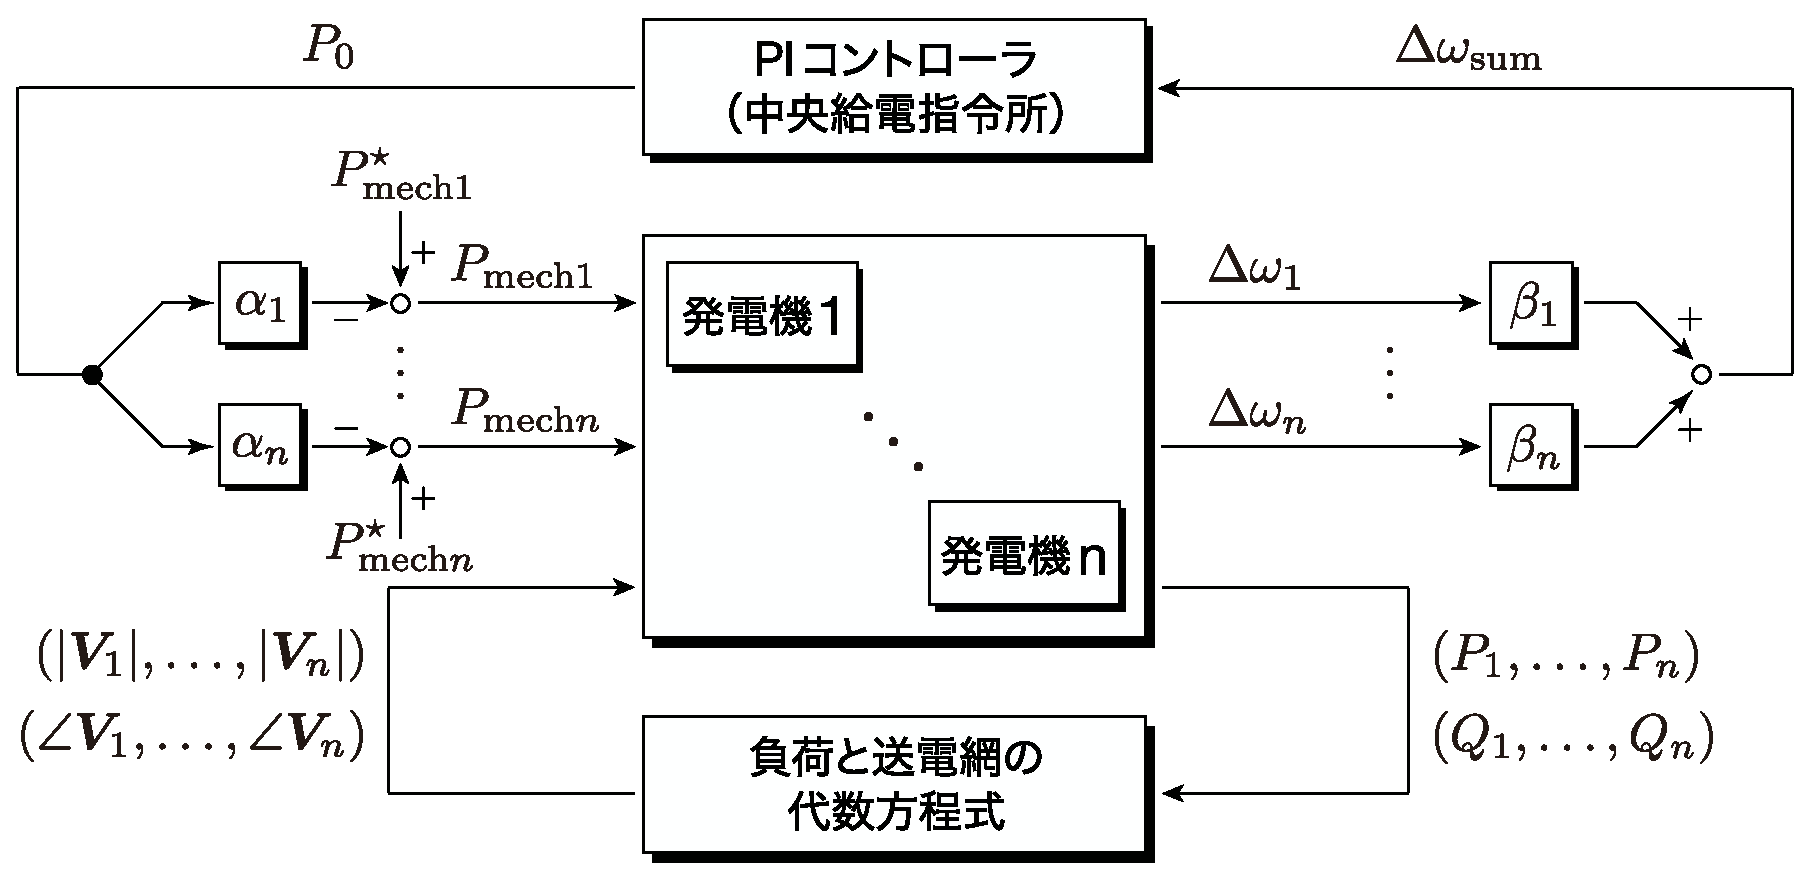
\includegraphics[width = .99\linewidth]{figs/bcAGC}
\medskip
\caption{\textbf{Signal transmission structure for automatic power generation control}}
\label{fig:bcAGC}
\medskip
\end{figure}

The automatic generation control (AGC) is a control algorithm that adjusts the
mechanical input $P_{{\rm mech}i}$ in Equation (\ref{eq:gendifagc}). Here, we
consider a broadcast-type PI controller that observes the weighted sum of
frequency deviations for all generators and sends a control input with
appropriate weighting to all generators. Specifically, for each $i \in
\mathcal{I}_{\rm G}$, we set:

\begin{subequations}\label{eq:agccon}
\begin{equation}\label{eq:agccona}
  P_{{\rm mech}i}(t)=
  P_{{\rm mech}i}^{\star} - \alpha_i
  \underbrace{
  \left\{
  k_{\rm P} \Delta \omega_{\rm sum}(t) +
  k_{\rm I}
  \int_0^t \Delta \omega_{\rm sum}(\tau) d \tau
  \right\}
  }_{P_{0}(t)}
\end{equation}
where $P_{{\rm mech}i}^{\star}$ is a constant representing the standard setting
value of the mechanical input. Moreover, $\alpha_i$ is a non-negative constant
specifying the contribution of generator $i$, and:

\[
  \Delta \omega_{\rm sum}(t) := 
  \sum_{i =1}^n \beta_i \Delta \omega_{i}(t)
\]
is the weighted sum of frequency deviations with non-negative weights $\beta_i$.
Furthermore, $k_{\rm P}$ and $k_{\rm I}$ are positive constants representing the
gains of the PI controller. This AGC controller has a structure where the
generated signal $P_0(t)$, which is produced by a single PI controller with
weighting of $\alpha_i$ and $\beta_i$, is simultaneously broadcasted to all
generators (Figure \ref{fig:bcAGC}). Note that Equation \ref{eq:agccona} can be
expressed as a differential equation as follows:

\begin{equation}
  \begin{aligned}
    \dot{\xi}&=  \Delta \omega_{\rm sum} \\
    P_{{\rm mech}i} &= P_{{\rm mech}i}^{\star} - \alpha_i \left(k_{\rm P} \Delta \omega_{\rm sum} +  k_{\rm I} \xi \right)
  \end{aligned}
\end{equation}
\end{subequations}

In electric power systems engineering, the non-negative constant $\alpha_i$ is
referred to as the \textbf{participation factor}\index{participation factor} of
generator $i$. It should be noted that in real-world thermal power generation
and nuclear power generation, there is a \textbf{prime mover}\index{prime mover}
that generates mechanical input by rotating a turbine using high-pressure steam
generated by thermal or nuclear power. The prime mover incorporates a
\textbf{governor}\index{governor} that automatically controls the rotation speed
of the generator. In order to analyze more realistic automatic generation
control, it is necessary to consider a prime mover model that takes input from
the central dispatch center as setpoint and outputs mechanical input to the
generator \cite[Chapter 3]{taniguchi2011power}.

By changing the ratio of participation factors, it is possible to adjust the
values of effective power supplied by each generator in a balanced steady-state
load flow condition. From the perspective of system control engineering, this
can be interpreted as "moving the stable equilibrium point of the power system
model by switching controllers." As analyzed in Chapter \ref{sec:staana}, the
stability of the power system depends on the choice of equilibrium point. The
total generation cost and transmission loss of the power system also depend on
the choice of equilibrium point. Therefore, appropriately switching the
participation factors according to the distribution of load can lead to improved
system stability and reduced economic costs.

In actual power system operation, the updating of participation factors is
typically done at intervals of several minutes to several tens of minutes
\cite[Section 11.1]{kundur1994power}. In the terminology of power system
engineering, the scheme for updating these participation factors is called
\textbf{economic load dispatching control} (EDC)\index{economic load dispatching
control}. The control algorithm that uses the participation factors as constants
during the updating interval is called \textbf{load frequency control}
(LFC)\index{load frequency control}. However, it should be noted that there may
be cases where there is no clear distinction between economic load dispatching
control and load frequency control in the literature, or where economic load
dispatching control is considered as a different scheme, so caution is
necessary.


\subsection{Numerical simulation of frequency stabilization control}

Let's verify the effectiveness of frequency stabilization control using a simple
example.

\begin{example}{Frequency stabilization by Automatic Generation Control}\label{ex:agcdemo}
Consider the power system model consisting of 3 busbars as discussed in Examples
\ref{ex:derY}, \ref{ex:pf3bus}, and \ref{ex:inires}. The physical constants of
the generators and transmission lines are set to the same values as in Example
\ref{ex:inires}, and the initial values of the internal states of the generators
are set to the steady-state values shown in Table \ref{table:genst13b}. In
addition, the field input is assumed to be constant at the values shown in Table
\ref{table:genst13b}.

The load at busbar 2 is set to a constant power model, and we consider a case
where the consumption of active power increases by 1\% from the initial
steady-state load flow condition. First, we show the time response of the
frequency deviation when there is no automatic generation control and the
mechanical input of the generators is constant at the values shown in Table
\ref{table:genst13b}, as shown in Figure \ref{fig:agcPdemo}(a). It can be seen
that the steady-state value of the frequency deviation does not become zero
because the supply and demand are not balanced due to the increased power
consumption by the load.

Next, we show the results when the broadcast-type PI controller of Equation
\ref{eq:agccon} is incorporated as automatic generation control, with the
parameters of the controller set to the values shown in Table
\ref{table:agcpara}(a), as shown in Figure \ref{fig:agcPdemo}(b). From this
figure, it can be seen that the frequency deviation hardly occurs even when the
consumption of load power changes, due to the effectiveness of automatic
generation control.
\end{example}


\begin{figure}[t]
  \centering
  {
  \begin{minipage}{0.49\linewidth}
    \centering
    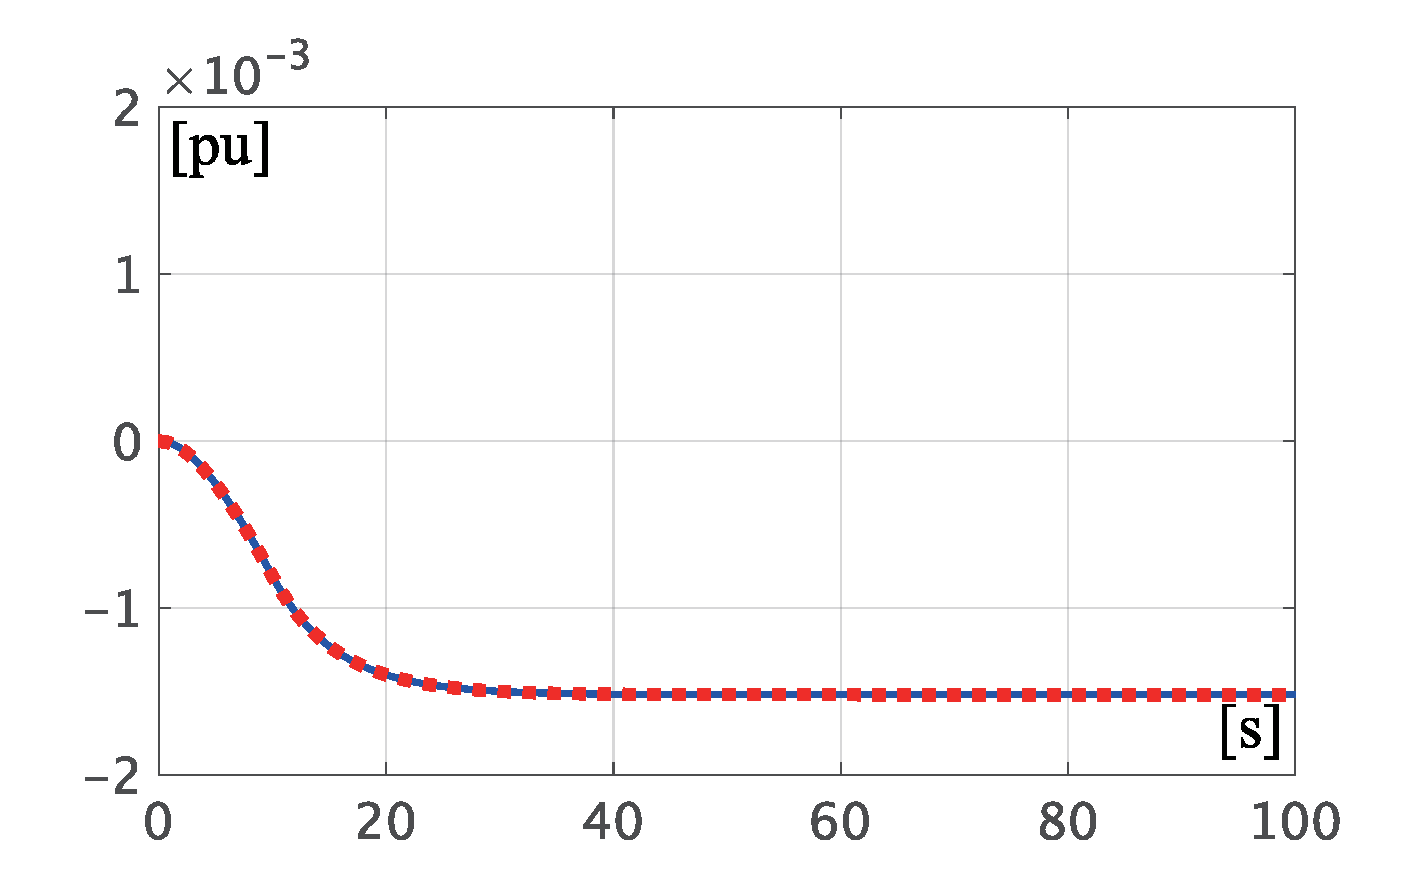
\includegraphics[width = 1.0\linewidth]{figs/woagcPinc}
    \subcaption{No automatic power generation control}
  \end{minipage}
  \begin{minipage}{0.49\linewidth}
    \centering
    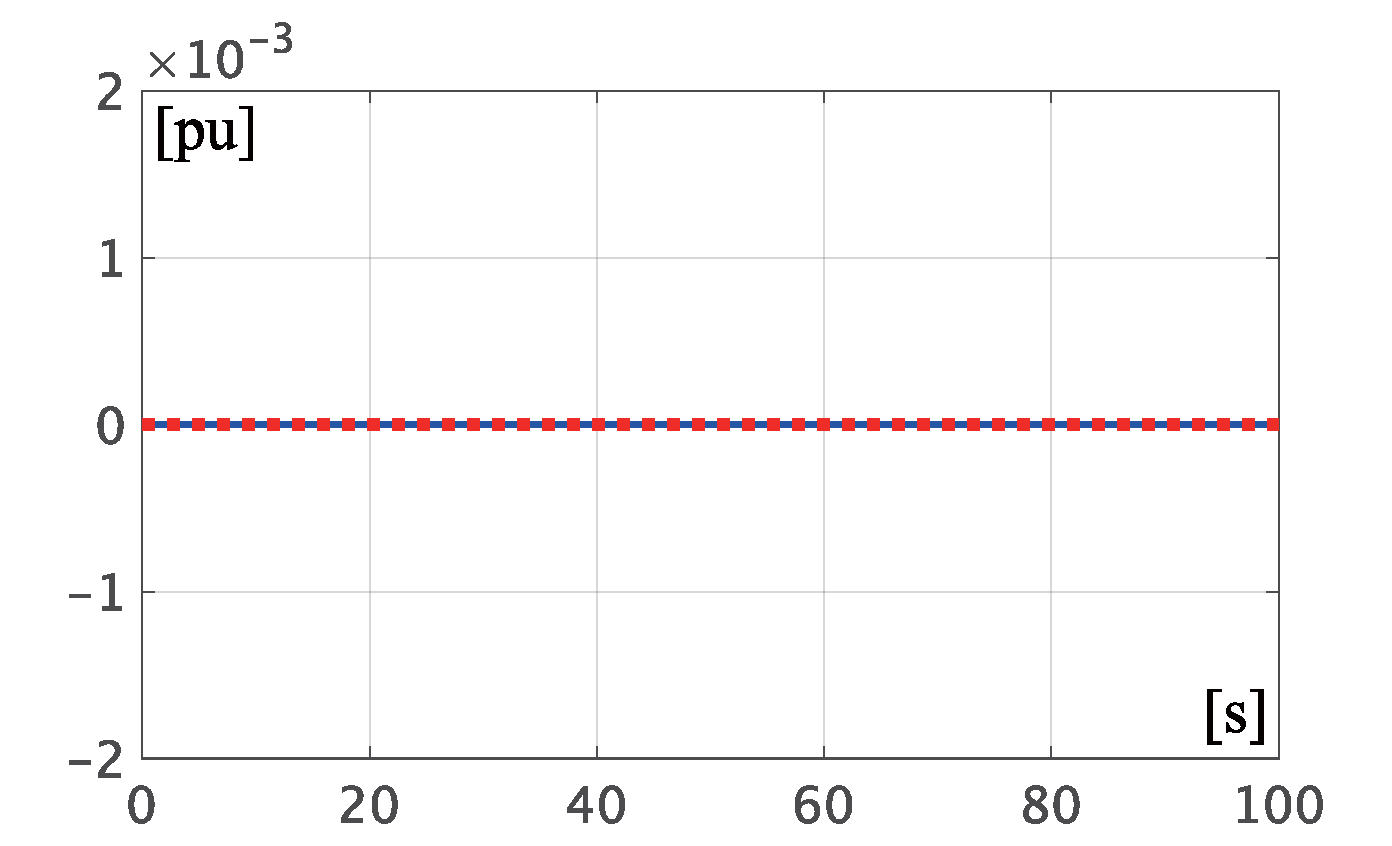
\includegraphics[width = 1.0\linewidth]{figs/wagcPinc}
    \subcaption{With automatic power generation control}
  \end{minipage}
  \medskip
  \caption{\textbf{Time response of angular frequency deviation to power consumption increase} 
    \\ \centering(Blue solid line: $Delta \omega_1$, Red dashed line: $Delta \omega_3$)}
  \label{fig:agcPdemo}
  }
\medskip
\end{figure}

\begin{table}[ht]
\medskip
 \caption{\textbf{Controller Parameter Setting}}
 \label{table:agcpara}
 \centering
  \begin{tabular}{ccccccccc}
   \hline
Setup &  $k_{\rm P}$ & $k_{\rm I}$ & $\alpha_1$ & $\alpha_3$ &$\beta_1$ & $\beta_3$ \\
   \hline \hline
(a) & 100 & 500 & 1 & 3 & 1 & 3 \\
(b) & 100 & 500 & 1 & 1& 1 & 1 \\
(c) & 100 & 500 & 3 & 1 & 3 & 1 \\
   \hline
  \end{tabular}
\end{table}

Next, let us confirm the change in steady-state power flow conditions by
adjusting the contribution coefficients of the broadcast-type PI controller in
Equation \ref{eq:agccon} to achieve supply-demand balance.

\begin{example}{Change in steady-state power flow conditions by adjusting contribution coefficients}\label{ex:pfvary}
Consider a power system model consisting of two generators and one load, similar
to Example \ref{ex:agcdemo}. Here, we confirm that the ratio of active power
supplied by Generator 1 and Generator 3 changes by varying the contribution
coefficients of the broadcast-type PI controller in Equation \ref{eq:agccon}.
Specifically, we switch the contribution coefficients as follows:

\begin{itemize}
\item Parameters of \ref{table:agcpara} (b) are set for 0 [s] to 20 [s].
\item Parameters of \ref{table:agcpara} (a) are set for 20 [s] to 40 [s].
\item Parameters of \ref{table:agcpara} (c) are set for 40 [s] to 60 [s].
\end{itemize}

The resulting time response is shown in Figure \ref{fig:agcPvary}(a). The solid
blue line represents the value of active power supplied by Generator 1 ($P_1$),
and the dashed red line represents the value of active power supplied by
Generator 3 ($P_3$). From this result, it can be seen that the ratio of $P_1$
and $P_3$ in the steady-state power flow conditions matches the ratio of
contribution coefficients $\alpha_1$ and $\alpha_3$.

Next, the time response of the total active power transmission loss
$P_1+P_2+P_3$, which represents the power transmission loss due to active power,
is shown in Figure \ref{fig:agcPvary}(b). Note that $P_2$ is the active power
consumed by the load and its value is constant at $-3$.

From this figure, it can be seen that the magnitude of active power transmission
loss varies depending on the realized steady-state power flow conditions. In
particular, when the parameters of the broadcast-type PI controller are set to
the values in Table \ref{table:agcpara} (a), i.e., when power is mainly supplied
using the lossless transmission line between Bus 2 and Bus 3, the total power
transmission loss of the entire power system is smaller, which is consistent
with the discussion in Example \ref{ex:pf3bus}. The admittance of the
transmission lines is set to the values in Equation (\ref{eq:rightlossless}).
\end{example}

\begin{figure}[t]
  \centering
  {
  \begin{minipage}{0.49\linewidth}
    \centering
    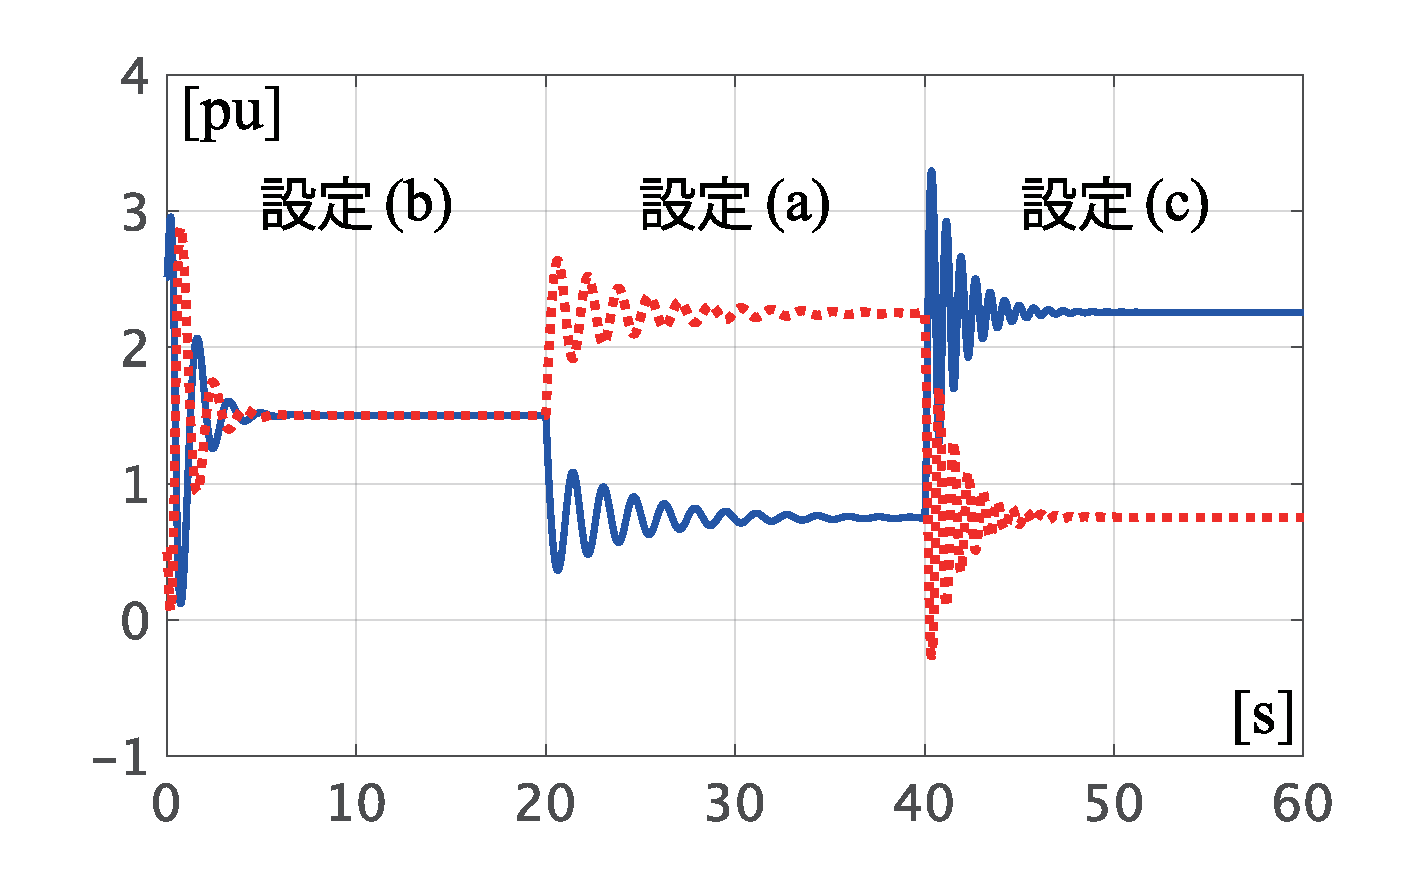
\includegraphics[width = 1.0\linewidth]{figs/varyalphaP}
    \subcaption{ Blue solid line: $P_1$, Red dashed line: $P_3$. }
  \end{minipage}
  \begin{minipage}{0.49\linewidth}
    \centering
    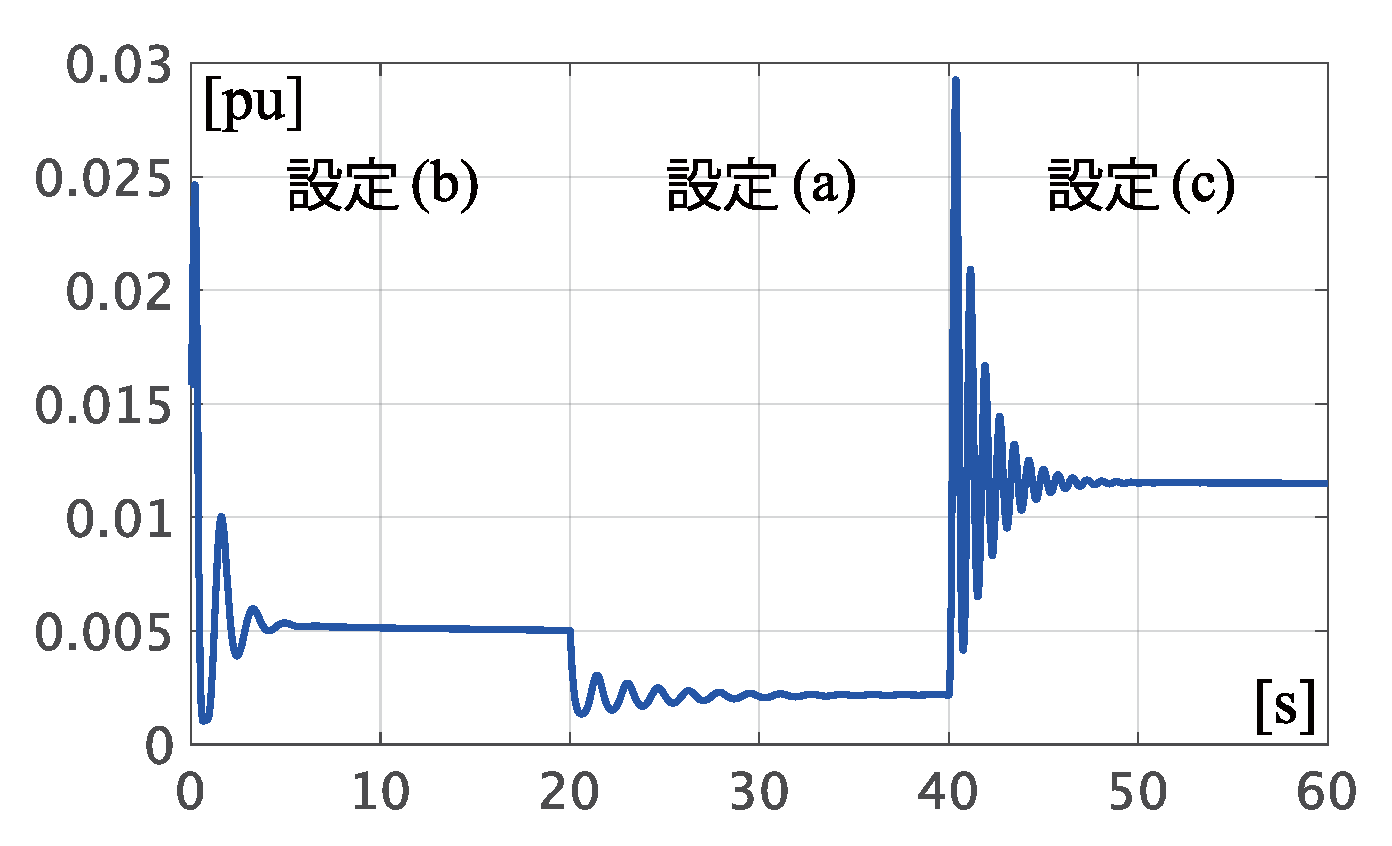
\includegraphics[width = 1.0\linewidth]{figs/varyalphaloss}
    \subcaption{Transmission loss $P_1+P_2+P_3$.}
  \end{minipage}
  \medskip
  \caption{\textbf{Time response of effective power to changes in contribution factor} }
  \label{fig:agcPvary}
  }
\medskip
\end{figure}

As shown in Example \ref{ex:pfvary}, by adjusting the contribution coefficients
of a broadcast-type PI controller, it is possible to change the steady-state
power flow condition. At the same time, the magnitude of transmission losses and
the required generation cost for each steady-state power flow condition also
change. Therefore, by appropriately controlling the contribution coefficients,
it is possible to achieve more economical system operation. However, it should
be noted that a steady-state power flow condition with lower economic costs is
not necessarily a highly stable equilibrium point, so it is important to
carefully consider trade-offs between economic efficiency and stability. 

\section{Mathematical stability analysis of frequency stabilization control
system}\label{sec:mathnpas}

\subsection{Power system model under consideration}\label{sec:objmod}

\smallskip
\subsubsection{Assumptions on Power System Model and Automatic Generation Control}

In Section \ref{sec:stalin}, an approximate linear model was derived under the
assumption that the power system model is in the vicinity of steady-state power
flow conditions, and necessary and sufficient conditions for steady-state
stability were analyzed. In this section, using the concept of passivity for
nonlinear systems, we analyze the frequency stability of the power system model
described as a system of differential-algebraic equations, taking into
consideration the stability of the entire feedback control system with automatic
generation control. Specifically, we conduct stability analysis under the
following assumptions.

\begin{itemize}
  \item All generators are expressed with the generator model of Equation
  (\ref{eq:lmodelsagc}). However, it is assumed that the field voltage of each
  generator is set to a constant.
  \item All loads are expressed with the constant power model of Equation
  \ref{eq:contpwmod}.
  \item For algebraic equations for the power grid of Equation
  \ref{eq:PQVgenagc}, conductance of all transmission lines is assumed to be 0.
  \item For the broadcast-type PI controller of Equation (\ref{eq:agccon}),
  automatic generation control is performed.
  However, it is assumed that $\alpha_i$ and $\beta_i$ are equal for all $i\in
  \mathcal{I}_{\rm G}$ for the weight of the participation factor and frequency
  deviation.
\end{itemize}

The first and second assumptions refer to considering a standard model for the
generator and load in the power system. The third assumption regarding the
transmission network implies that transmission losses are assumed to be zero,
which is essential for conducting stability analysis mathematically. In reality,
it is not possible to completely eliminate transmission losses in a power
system, but reducing transmission losses can be achieved by transmitting power
at higher voltages with lower currents. The discussion in this section assumes
that transmission losses can be approximately considered as zero due to
high-voltage transmission. The fourth assumption is necessary for the
input-output characteristics of the broadcast-type PI controller to be passive.
However, it should be noted that even if some coefficients are zero, as long as
at least one contribution coefficient $\alpha_i$ for $i\in \mathcal{I}_{\rm G}$
is positive, it is acceptable. 

Furthermore, as shown in the analysis of Section \ref{sec:phsync}:

\begin{itemize}
  \item The frequency deviation of all generators become equalize under a steady power flow distribution.
\end{itemize}

The following frequency stability analysis is based on this fact. Specifically,
in order for the integral controller in the broadcast-type PI controller to make
the steady-state angular frequency deviations of all generators zero, it is
necessary for the above-mentioned angular frequency deviations to automatically
synchronize with each other. Note that this requires the characteristic of
automatic synchronization among the angular frequency deviations using only one
integrator included in the broadcast-type PI controller.

\smallskip
\subsubsection{Representation of power system with automatic generation control
as a feedback system}

Similar to the discussion in Section \ref{sec:linpasana}, we consider
representing the power system model as a feedback system consisting of two
subsystems. The first subsystem is described by the following equations:
\begin{equation}\label{eq:sys1}
  \mathds{F}:
  \begin{aligned}
    M \Delta \dot{\omega}&= 
    - 
    D
    \Delta\omega 
    + 
    u_{\mathds{F}}
    +P_{{\rm mech}}^{\star}
    \\
    y_{\mathds{F}}&= \omega_0 \Delta\omega 
  \end{aligned}
\end{equation}

However, $\Delta\omega$ is a vector composed of $\Delta\omega_i$ stacked
vertically, and $M$ and $D$ are matrices formed by diagonally arranging $M_i$
and $D_i$. Also, $P_{{\rm mech}}^{\star}$ is a constant vector composed of
$P_{{\rm mech}i}^{\star}$. This $\mathds{F}$ is equivalent to the mechanical
subsystem in Section \ref{sec:linpasana}, except for the difference in the
constant vector $P_{{\rm mech}}^{\star}$. The second subsystem is represented by
the nonlinear differential-algebraic equation system of the electrical subsystem
in Section \ref{sec:linpasana}, given by:

\begin{subequations}\label{eq:sys2G}
\begin{equation}\label{eq:sys2}
  \mathds{G}_i : 
  \begin{aligned}
    \dot{\delta}_i &= u_{\mathds{G}_i}
    \\
    \taudi \dot{E}_i & = 
    -\tfrac{ \Xsi }{ \Xti }E_i
    +\left(
    \tfrac{ \Xsi }{ \Xti }-1
    \right)
    |\bm{V}_i| \sfcos (\delta_i - \angle \bm{V}_i ) 
    + V_{{\rm field}i}^{\star}
    \\
    y_{\mathds{G}_i}&= \tfrac{E_i |\bm{V}_i|}{ \Xti} \sfsin (\delta_i - \angle \bm{V}_i)
  \end{aligned}
\end{equation}

The voltage phasor of the bus in Equation \ref{eq:sys2} satisfies a set of
simultaneous equations for all generator buses as follows:

\begin{equation}\label{eq:gVeq}
  \begin{aligned}
    P_i &=
    \sum_{j=1}^{N} B_{ij} |\bm{V}_i| |\bm{V}_j| \sfsin(\angle \bm{V}_i -\angle \bm{V}_j)
    \\
    Q_i &= 
    -\sum_{j=1}^{N} B_{ij} |\bm{V}_i| |\bm{V}_j| \sfcos(\angle \bm{V}_i -\angle \bm{V}_j)
  \end{aligned}
  \qquad
  i \in \mathcal{I}_{\rm G}
\end{equation}
and a set of coupled equations for all load bus bars given by:

\begin{equation}\label{eq:lVeq}
  \simode{
    &P_{{\rm load}i}^{\star} =
    \sum_{j=1}^{N} B_{ij} |\bm{V}_i| |\bm{V}_j| \sfsin(\angle \bm{V}_i -\angle \bm{V}_j)
    \\
    &Q_{{\rm load}i}^{\star} = 
    -\sum_{j=1}^{N} B_{ij} |\bm{V}_i| |\bm{V}_j| \sfcos(\angle \bm{V}_i -\angle \bm{V}_j)
  }\qquad
  i \in \mathcal{I}_{\rm L}
\end{equation}
\end{subequations}

In addition, the active power $P_i$ and reactive power $Q_i$ in Equation
(\ref{eq:gVeq}) are defined by Equation (\ref{eq:PQoutagc}). Also, $B_{ij}$
represents the $(i,j)$ element of the susceptance matrix $B$, which is the
imaginary part of the admittance matrix $\bm{Y}$. In the following, we consider
the combination of Equations (\ref{eq:sys2}) to (\ref{eq:lVeq}) for all
generator buses $i \in \mathcal{I}_{\rm G}$ as one subsystem, and denote it as
the electrical subsystem $\mathds{G}$.

Furthermore, the dynamic characteristics of the broadcast-type PI controller in
Equation (\ref{eq:agccon}) are represented as follows:
\begin{equation}\label{eq:condsK}
  \mathds{K}: \simode{
  \dot{\xi}&=  h^{\sf T} u_{\mathds{K}} \\
  y_{\mathds{K}} &= h \left(k_{\rm P} h^{\sf T}u_{\mathds{K}} +  k_{\rm I} \xi \right)
  }
\end{equation}
where $h$ is a column vector consisting of $\alpha_i$.

In this case, the inputs and outputs of the aforementioned subsystems
$\mathds{F}$, $\mathds{G}$, and controller $\mathds{K}$ are interconnected as
follows:
\begin{subequations}\label{eq:connds}
\begin{align}
u_{\mathds{F}} = - y_{\mathds{K}} + v_{\mathds{F}}&
,\qquad u_{\mathds{K}} = \frac{1}{\omega_0} y_{\mathds{F}}	\label{eq:connds1}
\\
u_{\mathds{G}} = y_{\mathds{F}}&
,\qquad
v_{\mathds{F}} = - y_{\mathds{G}}		\label{eq:connds2}
\end{align}
\end{subequations}

This represents the entire feedback control system incorporating automatic
generation control. However, it should be noted that the "power balance
equation" block includes unknown model parameters such as load consumption power
and transmission line admittance. The block diagram of the entire feedback
control system is shown in Figure \ref{fig:nonlinBD}. Please note that the block
representing the "power balance equation" includes unknown model parameters such
as load consumption power and transmission line admittance.

\begin{figure}[t]
\centering
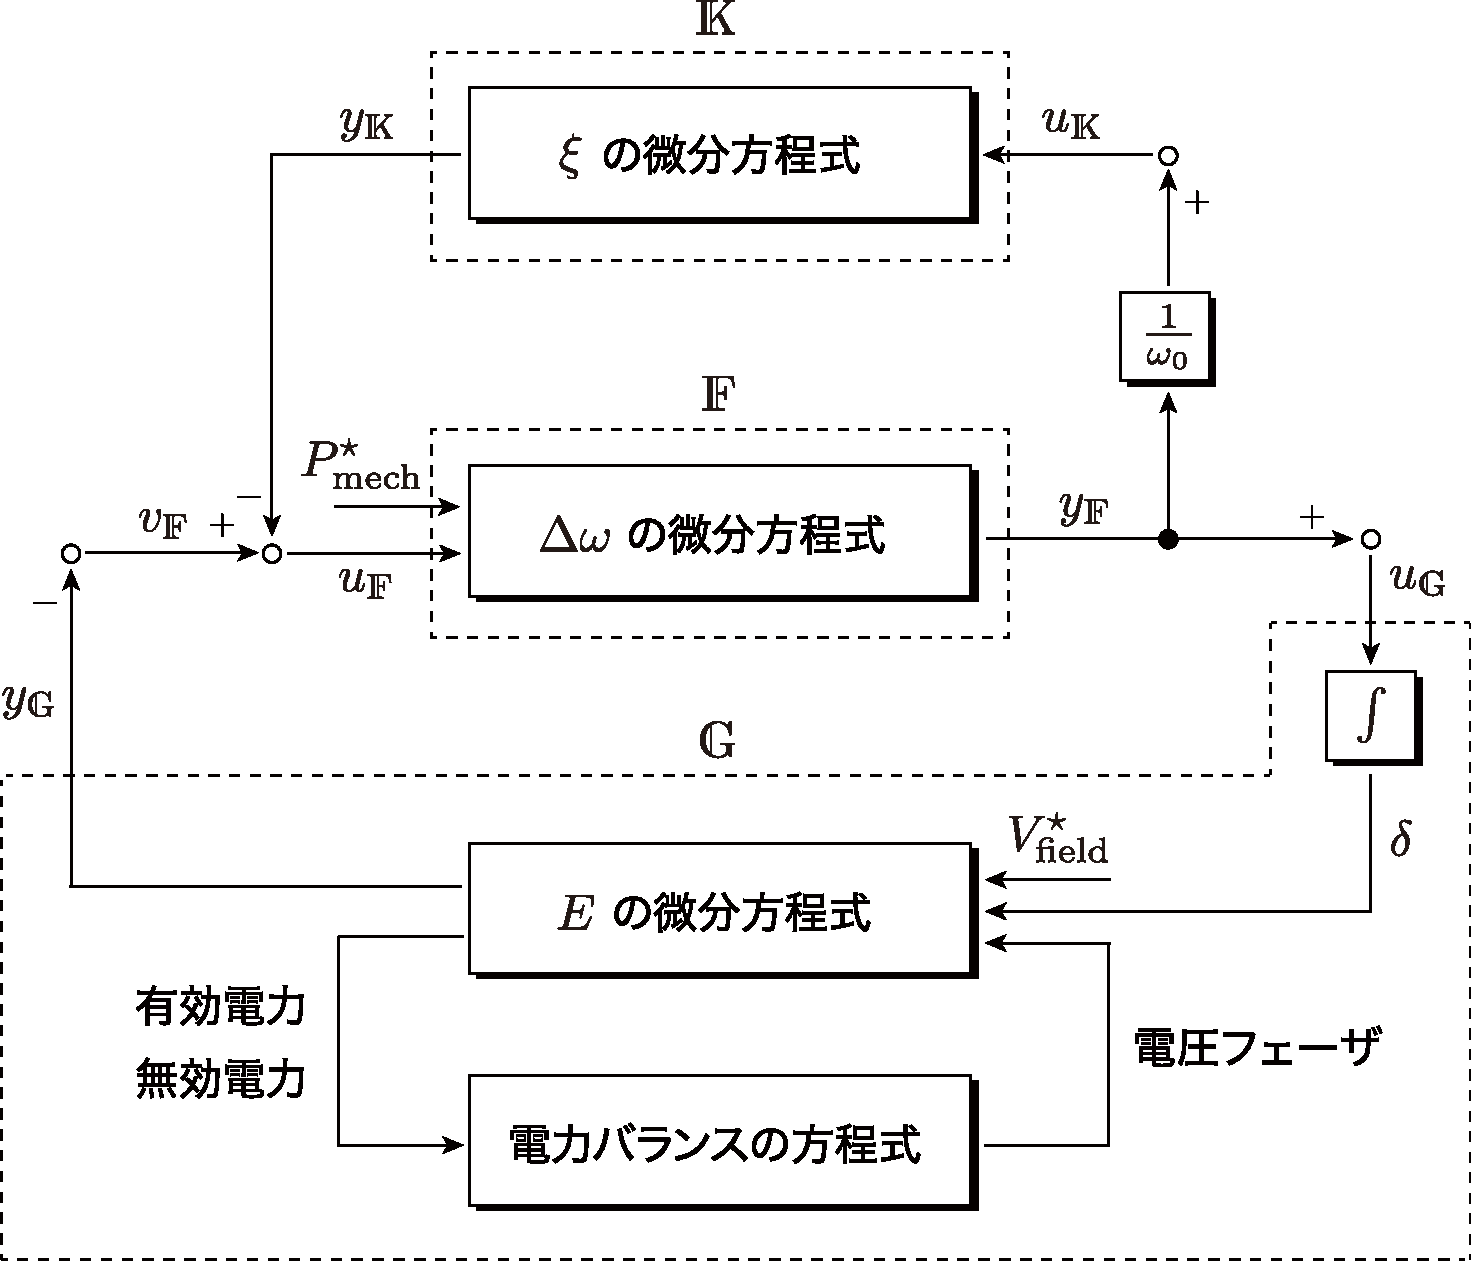
\includegraphics[width = .85\linewidth]{figs/nonlinBD}
\medskip
\caption{\textbf{Feedback control system incorporating automatic power generation control}}
\label{fig:nonlinBD}
\medskip
\end{figure}



\subsection{Equilibrium-independent passivity of power system models}

\smallskip
\subsubsection{Equilibrium-independent passivity}

The discussion in Section \ref{sec:linpasana} was based on an approximate linear
model, and the convergence to zero of the internal state represented the
asymptotic convergence to a specific steady-state power flow condition in the
original nonlinear model. On the other hand, in power system models represented
as nonlinear differential-algebraic equation systems, the internal state does
not necessarily converge to zero even at steady-state power flow conditions
where power supply and demand are balanced. Furthermore, the steady-state power
flow condition itself can change depending on set values such as mechanical
inputs. Therefore, it is desirable to conduct stability analysis that does not
depend on the selection of individual steady-state power flow conditions
(equilibrium points). A concept proposed in control engineering for such
analysis is called \textbf{equilibrium-independent
passivity}\index{equilibrium-independent passivity}
\cite{hines2011equilibrium,simpson2019equilibrium}.  Note that in some
literature, it is also referred to as \textbf{shifted passivity}\index{shifted
passivity} \cite{monshizadeh2019conditions}.  Its definition is given as
follows.

\begin{definition}[Equilibrium-independent passivity]\label{def:eipassive}
Let us consider a nonlinear system:

\begin{equation}\label{eq:nlsig}
  \Sigma: \simode{
  E\dot{x} &= f(x) + Bu + R d^{\star}\\
  y &= h(x)
  }
\end{equation}
where $f:\mathcal{X} \rightarrow \mathbb{R}^{n}$ and $h:\mathcal{X} \rightarrow
\mathbb{R}^{m}$ are smooth functions, and $B \in \mathbb{R}^{n\times m}$, $E \in
\mathbb{R}^{n\times n}$, $R \in \mathbb{R}^{n\times p}$ are matrices. Also,
$d^{\star}\in \mathbb{R}^p$ is a constant vector. Here, $\mathcal{X}$ represents
the admissible state space.

The set of achievable equilibrium points by constant inputs is denoted as:

\begin{equation*}%\label{eq:asbleq}
  \mathcal{E}_{\Sigma} :=
  \left\{
  x^{\star} \in \mathcal{X}: 
  \mbox{there exists $u^{\star}$ satisfying $0 = f(x^{\star})+B u^{\star}+ R d^{\star}$}
  \right\}
\end{equation*}

For each equilibrium point $x^{\star} \in \mathcal{E}{\Sigma}$, if there exists
a differentiable positive semi-definite function $W{x^{\star}}:\mathcal{X}
\rightarrow \mathbb{R}{\geq 0}$ such that $W{x^{\star}} (x^{\star}) = 0$ and for
any input $u$, the following inequality holds for all $t \geq 0$:

\begin{equation*}%\label{eq:eiconpv}
  \frac{d}{dt} W_{x^{\star}} \bigl( x(t) \bigr) \leq \bigl(u(t)-u^{\star}\bigr)^{\sf T} \bigl(y(t)-y^{\star}\bigr)
  ,\qquad
  \forall t \geq 0
\end{equation*}
then $\Sigma$ is called \textbf{equilibrium-independent passive}. Here,
$u^{\star}$ and $y^{\star}$ denote the steady-state input and output at the
equilibrium point, respectively, and are defined as:

\begin{equation*}%\label{eq:uystar}
  u^{\star} := -(B^{\sf T}B)^{-1}B^{\sf T} \bigl\{f(x^{\star}) + R d^{\star} \bigr\}
  ,\qquad
  y^{\star} := h(x^{\star}) 
\end{equation*}

In particular, if there exists a positive constant $\rho$ such that the
following inequality holds for all $t \geq 0$:

\begin{equation*}%\label{eq:eiconosp}
  \frac{d}{dt} W_{x^{\star}} \bigl( x(t) \bigr) \leq \bigl(u(t)-u^{\star}\bigr)^{\sf T} \bigl(y(t)-y^{\star}\bigr)
  -\rho \bigl\|y(t)-y^{\star} \bigr\|^2
  ,\qquad
  \forall t \geq 0
\end{equation*}
then $\Sigma$ is called \textbf{equilibrium-independent strictly passive}.
\end{definition}

In Definition \ref{def:eipassive}, the passivity of the system is defined with
respect to the equilibrium point $x^{\star} \in \mathcal{E}{\Sigma}$ as a
reference. In the context of linear systems, it is known that this definition of
passivity is equivalent to the definition of passivity in Section
\ref{sec:linpasana}, unless the system has a zero eigenvalue
\cite{hines2011equilibrium}. Note that the function $W_{x^{\star}}(x)$ mentioned
above is called the storage function, similar to conventional passivity
definitions. It should be noted that this storage function $W_{x^{\star}}(x)$ is
an implicit function of the equilibrium point $x^{\star}$.

\begin{COLUMN}
\noindent \textbf{Descriptor representation}:
The matrix $E$ in Equation \ref{eq:nlsig} is introduced to represent the
electrical subsystem $\mathds{G}$ of the differential-algebraic equation system
given by Equation (\ref{eq:sys2G}). Specifically, by setting:

\[
  E=\mat{
  I & 0 \\
  0 & 0\\ 
  }
\]
the system $\Sigma$ in Equation \ref{eq:nlsig} represents the following
differential-algebraic equation system:

\begin{equation*}
  \simode{
    \dot{x}_1 &= f_1(x_1,x_2) + B_1u + R_1 d^{\star}\\
    0 &= f_2(x_1,x_2) \\
    y &= h(x_1,x_2)
  }
\end{equation*}

When applied to the electrical subsystem $\mathds{G}$, $x_1$ is a vector
containing all $\delta_i$ and $E_i$, and $x_2$ is a vector containing all
$|\bm{V}_i|$ and $\angle \bm{V}_i$. On the other hand, when $E$ is regular, it
represents a differential equation system like the mechanical subsystem
$\mathds{F}$ given by Equation \ref{eq:sys1}. This type of system
representation is called the \textbf{descriptor representation}.
\end{COLUMN}

In reference \cite{simpson2019equilibrium}, it is shown that when a system is
passive regardless of its equilibrium point, its storage function can be
expressed in the form of Equation \ref{eq:paraW} using a certain function
$U(x)$:

\begin{equation}\label{eq:paraW}
  W_{x^{\star}}(x) = U(x) - U(x^{\star}) - \nabla U^{\sf T}(x^{\star}) (x-x^{\star})
\end{equation}

In Definition \ref{def:eipassive}, it is a requirement that the storage function
$W_{x^{\star}}(x)$ in Equation \ref{eq:paraW} is a positive semi-definite
function. Specifically, the condition is that Equation \ref{eq:Uineqst} holds:

\begin{equation}\label{eq:Uineqst}
  U(x) \geq  U(x^{\star}) + \nabla U^{\sf T}(x^{\star}) (x-x^{\star})
\end{equation}

If this inequality holds for any pair $(x,x^{\star}) \in \mathcal{X} \times
\mathcal{X}$, then for each equilibrium point $x^{\star} \in
\mathcal{E}{\Sigma}$, $W{x^{\star}}(x)$ is a positive semi-definite function.
The inequality in Equation \ref{eq:Uineqst} expresses the convexity of the
function $U(x)$. As will be explained later, the region $\mathcal{X}$ where
$U(x)$ is convex plays an important role in stability analysis using passivity
that does not depend on the equilibrium point.

\begin{COLUMN}
\noindent \textbf{Convex function}:
A function $f(x)$ is called \textbf{convex} if, for any two points $(x,y)$ in
its domain and any $\theta \in [0,1]$, the following inequality holds:

\[
  f\bigl(
  \theta x + (1-\theta) y
  \bigr)
  \leq \theta f(x) + (1- \theta) f(y)
  ,\qquad
  \forall \theta \in [0,1]
\]

In particular, if $f(x)$ is differentiable, a necessary and sufficient condition
for $f(x)$ to be convex is that, for any two points $(x,y)$,

\[
  f(x) \geq f(y) + \nabla f^{\sf T}(y)(x-y)
\]

This inequality means that the graph of $f(x)$ is always above the tangent line
to $f(x)$ at the point $x=y$.

\smallskip
\noindent \textbf{Bregman Distance}:
In statistics, the quantity on the right-hand side of equation \ref{eq:paraW}
for a convex function $U(x)$ is called the \textbf{Bregman distance}
\cite{bregman1967relaxation} between $x$ and $x^{\star}$ with respect to $U(x)$.
If $U(x)$ is chosen to be $|x|^2$, then the Bregman distance $W_{x^{\star}}(x)$
reduces to the Euclidean distance $|x-x^{\star}|^2$.
\end{COLUMN}

\smallskip
\subsubsection{Analysis of the mechanical subsystem}

As shown in Section \ref{sec:linpasana}, the mechanical subsystem $\mathds{F}$
is strongly passive. Similarly, we confirm that $\mathds{F}$ in Equation
\ref{eq:sys1} is also strongly passive regardless of the equilibrium point.
First, the mechanical subsystem is represented in the form:

\begin{equation}
  \mathds{F}: \simode{
  \dot{x}_{\mathds{F}} & = A_{\mathds{F}} x_{\mathds{F}} + B_{\mathds{F}} u_{\mathds{F}} 
  + R_{\mathds{F}} d_{\mathds{F}}^{\star} \\
  y_{\mathds{F}} &= C_{\mathds{F}} x_{\mathds{F}}
  }
\end{equation}

Here, the state $x_{\mathds{F}}$ is a vector consisting of $\Delta \omega_i$,
and $u_{\mathds{F}}$ and $y_{\mathds{F}}$ are vectors consisting of
$u_{\mathds{F}i}$ and $y{\mathds{F}i}$, respectively. Also,
$d{\mathds{F}}^{\star}$ represents $P_{\rm mech}^{\star}$, and the system
matrices are:

\[
  A_{\mathds{F}} := -M^{-1}D,\qquad
  B_{\mathds{F}} := M^{-1},\qquad
  R_{\mathds{F}} := M^{-1},\qquad
  C_{\mathds{F}} := \omega_0 I
\]

Note that the matrices $M$ and $D$ are diagonal matrices composed of $M_i$ and
$D_i$. For an arbitrarily selected equilibrium point $x^{\star}{\mathds{F}} \in
\mathcal{E}{\mathds{F}}$, the storage function is chosen as:

\begin{equation}\label{eq:WxFst}
W_{x^{\star}_{\mathds{F}}}(x_{\mathds{F}})
= \frac{\omega_0}{2}
(x_{\mathds{F}} -x^{\star}_{\mathds{F}})^{\sf T}
M
(x_{\mathds{F}} -x^{\star}_{\mathds{F}})
\end{equation}

Here, $(x^{\star}{\mathds{F}},u^{\star}{\mathds{F}},y^{\star}{\mathds{F}})$ with
respect to the equilibrium point satisfies:

\begin{equation}\label{eq:xFsteady}
  0=
  A_{\mathds{F}} x^{\star}_{\mathds{F}}
  +
  B_{\mathds{F}} u^{\star}_{\mathds{F}}
  + R_{\mathds{F}} d_{\mathds{F}}^{\star}
  ,\qquad
  y^{\star}_{\mathds{F}} = C_{\mathds{F}} x^{\star}_{\mathds{F}}
\end{equation}

If expressed in the form of Equation \ref{eq:paraW}, the storage function can be
written as:

\[
  U_{\mathds{F}}(x_{\mathds{F}}):= \frac{\omega_0}{2} x_{\mathds{F}}^{\sf T} M x_{\mathds{F}}
\]

Therefore, the storage function can be expressed as:

\[
  W_{x^{\star}_{\mathds{F}}}(x_{\mathds{F}}) = U_{\mathds{F}}(x_{\mathds{F}}) 
  - U_{\mathds{F}}(x^{\star}_{\mathds{F}}) 
  - \nabla U^{\sf T}_{\mathds{F}}(x^{\star}_{\mathds{F}}) (x_{\mathds{F}}-x^{\star}_{\mathds{F}})
\]

The gradient function of this storage function can be expressed as:

\begin{equation*}%\label{eq:nabW}
  \nabla W_{x^{\star}_{\mathds{F}}}(x_{\mathds{F}}) = \omega_0 M (x_{\mathds{F}} -x^{\star}_{\mathds{F}})
\end{equation*}

Hence, the time derivative of the storage function can be evaluated as:

\begin{equation}\label{eq:tdFds}
  \spliteq{
    \frac{d}{dt} W_{x^{\star}_{\mathds{F}}} \bigl( x_{\mathds{F}}(t) \bigr) 
    &= 
    \nabla W_{x^{\star}_{\mathds{F}}}^{\sf T}\left( x_{\mathds{F}}(t) \right) \dot{x}_{\mathds{F}}(t) \\
    &= 
    \nabla W_{x^{\star}_{\mathds{F}}}^{\sf T}\left( x_{\mathds{F}}(t) \right)
    \left\{
    A_{\mathds{F}} \left( x_{\mathds{F}}(t) -x^{\star}_{\mathds{F}} \right)
    +
    B_{\mathds{F}} \left( u_{\mathds{F}}(t) -u^{\star}_{\mathds{F}} \right)
    \right\}
    \\
    & \leq \textstyle
    (y_{\mathds{F}}(t) -y^{\star}_{\mathds{F}})^{\sf T}
    (u_{\mathds{F}}(t) -u^{\star}_{\mathds{F}})
    - \tfrac{\sfmin \left\{ D_i \right\}}{\omega_0}
    \|y_{\mathds{F}}(t) -y^{\star}_{\mathds{F}}\|^2
  }
\end{equation}

Here, the derivation of the second equality used the relationship in Equation \ref{eq:xFsteady}.

\smallskip
\subsubsection{Analysis of feedback system for mechanical subsystem and automatic power generation controller}

Similar to the mechanical subsystem, the passivity of the broadcast-type PI
controller in equation \ref{eq:condsK} can also be demonstrated. By defining the
storage function as:

\begin{equation}\label{eq:Wxist}
  W_{\xi^{\star}}(\xi) := \frac{1}{2} k_{\rm I} (\xi-\xi^{\star} )^2
\end{equation}
its time derivative can be evaluated as:

\begin{equation}\label{eq:tdKds}
  \spliteq{
    \frac{d}{dt} W_{\xi^{\star}} \bigl( \xi(t) \bigr) 
    &=
    (y_{\mathds{K}} - y_{\mathds{K}}^{\star})^{\sf T} (u_{\mathds{K}} - u_{\mathds{K}}^{\star})
    - k_{\rm P} u_{\mathds{K}}^{\sf T} hh^{\sf T} u_{\mathds{K}} \\
    & \leq (y_{\mathds{K}} - y_{\mathds{K}}^{\star})^{\sf T} (u_{\mathds{K}} - u_{\mathds{K}}^{\star})
  }
\end{equation}
where $(\xi^{\star},u_{\mathds{K}}^{\star},y_{\mathds{K}}^{\star})$ represents
the equilibrium point and Equation \ref{eq:Kdseq} is used. 

\begin{equation}\label{eq:Kdseq}
  \simode{
    0 &=  h^{\sf T} u_{\mathds{K}}^{\star} \\
    y_{\mathds{K}}^{\star} &= h \left(k_{\rm P} h^{\sf T}u_{\mathds{K}}^{\star} +  k_{\rm I} \xi^{\star} \right)
  }
\end{equation}

In system control engineering, it is known that a negative feedback system
between two passive systems becomes passive again. Based on this fact, a
feedback connection is made between the mechanical subsystem $\mathds{F}$ in
Equation \ref{eq:sys1} and the broadcast-type PI controller $\mathds{K}$ in
Equation \ref{eq:condsK}, resulting in the system:

\begin{equation}\label{eq:sysFKds}
  \mathds{F}_+:
  \simode{
    M \Delta \dot{\omega}&= 
    - 
    D
    \Delta\omega 
    - h \left(k_{\rm P} h^{\sf T}\Delta\omega  +  k_{\rm I} \xi \right)  + P_{{\rm mech}}^{\star} + v_{\mathds{F}}
    \\
    \dot{\xi} &= h^{\sf T}\Delta\omega\\
    y_{\mathds{F}}&= \omega_0 \Delta\omega 
  }
\end{equation}
which is strongly passive regardless of the equilibrium point. In fact, adding
the inequalities in Equation \ref{eq:tdFds} and Equation \ref{eq:tdKds}, we
obtain:

\begin{equation}\label{eq:disineqFp}
  \spliteq{
    & \frac{d}{dt}  \left\{
    W_{x^{\star}_{\mathds{F}}}  \bigl( x_{\mathds{F}}(t) \bigr) 
    +
    \omega_0
    W_{\xi^{\star}} \bigl( \xi(t) \bigr) 
    \right\} \\
    & \hspace{3em} \leq 
    (y_{\mathds{F}}(t) -y^{\star}_{\mathds{F}})^{\sf T}
    (v_{\mathds{F}}(t) -v^{\star}_{\mathds{F}})  
    - \tfrac{\sfmin \left\{ D_i \right\}}{\omega_0}
    \|y_{\mathds{F}}(t) -y^{\star}_{\mathds{F}}\|^2
  }
\end{equation}
where Equation \ref{eq:connds1} is used for the input-output relationship.

Furthermore, by using the input-output relationship in equation
\ref{eq:connds2}, combining the machine subsystem $\mathds{F}_+$ in equation
\ref{eq:sysFKds} with $\mathds{G}$ in equation \ref{eq:sys2G} represents the
entire feedback control system incorporating automatic generation control. Based
on this fact, we analyze the passivity of $\mathds{G}$ independent of the
equilibrium point below.

\smallskip
\subsubsection{Analysis of the electrical subsystem}

We analyze the passivity of the electrical subsystem $\mathds{G}$ in equation
(\ref{eq:sys2G}) independent of its equilibrium point. Here, we represent the
column vector containing the time-varying variables $\delta_i$, $E_i$,
$|\bm{V}_i|$, and $\angle \bm{V}i$ related to the generator bus and load bus of
$\mathds{G}$ as $x{\mathds{G}}$. Under this notation, we define the potential
energy function as follows:

\begin{equation}\label{eq:potWx}
  \spliteq{
    U_{\mathds{G}}(x_{\mathds{G}})  := 
    &  \sum_{i=1}^n
    \left\{
    \frac{ \Xsi E_i^2 }{2 \Xti ( \Xsi - \Xti )}  
    - 
    \frac{E_i |\bm{V}_i|}{ \Xti } \sfcos (\delta_i - \angle \bm{V}_i)
    +\frac{|\bm{V}_i|^2}{2 \Xti }
    \right\}
    \\
    - & 
    \sum_{i=n+1}^{n+m}
    \left\{
    P_{{\rm load}i}^{\star} \angle \bm{V}_i
    + Q_{{\rm load}i}^{\star} \ln \left|\bm{V}_i \right|
    \right\} \\
    - & \sum_{i=1}^{N}
    \sum_{j=1}^{N} \frac{B_{ij} }{2} |\bm{V}_i| |\bm{V}_j| \sfcos(\angle \bm{V}_i -\angle \bm{V}_j)
  }
\end{equation}

This potential energy function has been used, for example, in the stability
analysis of power systems consisting of a single-axis generator model and a
constant power load model, as described in
\cite{tsolas1985structure,varaiya1985direct,chiang2011direct}. Based on the
expression in Equation (\ref{eq:paraW}), a candidate storage function is
constructed as follows:

\begin{equation}\label{eq:stops}
  W_{x^{\star}_{\mathds{G}}}(x_{\mathds{G}}) = U_{\mathds{G}}(x_{\mathds{G}}) 
  - U_{\mathds{G}}(x^{\star}_{\mathds{G}}) 
  - \nabla U_{\mathds{G}}^{\sf T}(x^{\star}_{\mathds{G}}) (x_{\mathds{G}}-x^{\star}_{\mathds{G}})
\end{equation}

Its gradient function is:

\[
  \nabla W_{x^{\star}_{\mathds{G}}}(x_{\mathds{G}}) =
  \nabla U_{\mathds{G}}(x_{\mathds{G}}) 
  - \nabla U_{\mathds{G}}(x^{\star}_{\mathds{G}}) 
\]

To calculate the time derivative of the storage function, we need to find the
gradient function of the potential energy function. First, we calculate the
partial derivatives of $U_{\mathds{G}}(x_{\mathds{G}})$ with respect to
$\delta_i$ and $E_i$, which are given by:

\begin{equation*}
  \begin{aligned}
    \frac{\partial U_{\mathds{G}}}{\partial \delta_i}(x_{\mathds{G}}) &= \frac{E_i |\bm{V}_i|}{ \Xti } \sfsin (\delta_i - \angle \bm{V}_i) ,
    \\
    \frac{\partial U_{\mathds{G}}}{\partial E_i} (x_{\mathds{G}})&= - \frac{1}{ \Xsi - \Xti }
    \left\{
    -\frac{ \Xsi }{ \Xti }E_i
    +\left(
    \frac{ \Xsi }{ \Xti }-1
    \right)
    |\bm{V}_i| \sfcos (\delta_i - \angle \bm{V}_i ) 
    \right\}
  \end{aligned}
\end{equation*}

Therefore, if each variable follows the differential-algebraic equation of
Equation (\ref{eq:sys2G}), because of Equation \ref{eq:sys2}, the following is
true for all $i\in \mathcal{I}_{\rm G}$:

\begin{equation*}
\frac{\partial U_{\mathds{G}}}{\partial \delta_i}(x_{\mathds{G}})  = y_{\mathds{G}_i}
,\qquad
\frac{\partial U_{\mathds{G}}}{\partial E_i} (x_{\mathds{G}})= 
\frac{V_{{\rm field}i}^{\star} - \taudi\dot{E}_i  }{ \Xsi - \Xti }
\end{equation*}

The partial derivatives of the potential energy function with respect to the
voltage phase variables for $i\in \mathcal{I}_{\rm G}$ are given by:

\begin{equation*}
  \spliteq{
    \frac{\partial U_{\mathds{G}}}{\partial |\bm{V}_i| }(x_{\mathds{G}}) &= 
    -
    \sum_{j=1}^{N} B_{ij}  |\bm{V}_j| \sfcos(\angle \bm{V}_i -\angle \bm{V}_j)- \frac{Q_i}{|\bm{V}_i|}
    \\
    \frac{\partial U_{\mathds{G}}}{\partial \angle \bm{V}_i } (x_{\mathds{G}})&= 
    \sum_{j=1}^{N}
    B_{ij} |\bm{V}_i| |\bm{V}_j| \sfsin(\angle \bm{V}_i -\angle \bm{V}_j)
    -
    P_i
  }
\end{equation*}

Therefore, from Equation \ref{eq:gVeq}, it can be seen that these are equal to
0. Similarly, from Equation \ref{eq:lVeq}, for $i\in \mathcal{I}_{\rm L}$, it
can be seen that:

\begin{equation*}
\spliteq{
\frac{\partial U_{\mathds{G}}}{\partial |\bm{V}_i| }(x_{\mathds{G}}) &= 
- \sum_{j=1}^{N} B_{ij}  |\bm{V}_j| \sfcos(\angle \bm{V}_i -\angle \bm{V}_j)
 -  \frac{Q_{{\rm load}i}^{\star}}{|\bm{V}_i|}
\\
\frac{\partial U_{\mathds{G}}}{\partial \angle \bm{V}_i } (x_{\mathds{G}})&= 
\sum_{j=1}^{N} B_{ij} |\bm{V}_i| |\bm{V}_j| \sfsin(\angle \bm{V}_i -\angle \bm{V}_j)
-
P_{{\rm load}i}^{\star}
}
\end{equation*}

Therefore, it can be seen that for all $i\in \mathcal{I}_{\rm G} \cup \mathcal{I}_{\rm L}$:

\begin{equation*}
  \frac{\partial U_{\mathds{G}}}{\partial |\bm{V}_i| } (x_{\mathds{G}})= 0
  ,\qquad
  \frac{\partial U_{\mathds{G}}}{\partial \angle \bm{V}_i } (x_{\mathds{G}})= 0
\end{equation*}

\begin{subequations}\label{eq:eqeq}

Next, consider the set
$(x^{\star}_{\mathds{G}},u^{\star}_{\mathds{G}},y^{\star}_{\mathds{G}})$ related
to the steady-state of $\mathds{G}$ with respect to $\nabla
U{\mathds{G}}(x^{\star}{\mathds{G}})$. From the equilibrium condition, there
exists a set of voltage phasors $(|\bm{V}_i^{\star}|, \angle
\bm{V}_i^{\star})_{i\in \mathcal{I}_{\rm G} \cup \mathcal{I}_{\rm L} }$ such
that:

\begin{equation}\label{eq:eqeqa}
  \begin{aligned}
    &\simode{
    0 & = u_{\mathds{G}_i}^{\star} \\
    0 & =
    -\tfrac{ \Xsi }{ \Xti }E_i^{\star}
    +\left(
    \tfrac{ \Xsi }{ \Xti }-1
    \right)
    |\bm{V}_i^{\star}| \sfcos (\delta_i^{\star} - \angle \bm{V}_i^{\star} ) 
    +V_{{\rm field}i}^{\star}
    } \\
    &\simode{
    P_i^{\star} 
    & =
    \sum_{j=1}^{N} B_{ij} |\bm{V}_i^{\star}| |\bm{V}_j^{\star}| \sfsin(\angle \bm{V}_i^{\star} -\angle \bm{V}_j^{\star})
    \\
    Q_i^{\star} 
    &=
    - \sum_{j=1}^{N} B_{ij} |\bm{V}_i^{\star}| |\bm{V}_j^{\star}| \sfcos(\angle \bm{V}_i^{\star} -\angle \bm{V}_j^{\star})
    }
  \end{aligned}
\end{equation}

However, $i \in \mathcal{I}_{\rm G}$ and the steady-state values of active and
reactive power are:

\begin{equation*}%\label{eq:PQoutagcst}
  P_i^{\star}  :=  \frac{E_i^{\star}  |\bm{V}_i^{\star} |}{ \Xti } 
  \sfsin (\delta_i^{\star}  - \angle \bm{V}_i^{\star} ), \qquad
  Q_i^{\star}  :=  \frac{ E_i^{\star} |\bm{V}_i^{\star} | }{ \Xti } 
  \sfcos (\delta_i^{\star}  - \angle \bm{V}_i^{\star} )
  -\frac{|\bm{V}_i^{\star} |^2}{ \Xti }
\end{equation*}

In addition, $y_{\mathds{G}_i}^{\star}$ represents $P_i^{\star}$. Therefore,
the following holds for $ i \in \mathcal{I}_{\rm G} $:

\begin{equation*}
  \frac{\partial U_{\mathds{G}}}{\partial \delta_i}(x^{\star}_{\mathds{G}}) = y_{\mathds{G}_i}^{\star}
  ,\qquad
  \frac{\partial U_{\mathds{G}}}{\partial E_i}(x^{\star}_{\mathds{G}}) = 
  \frac{V_{{\rm field}i}^{\star}  }{ \Xsi - \Xti }
\end{equation*}

Similarly, since the following holds for all $ i \in \mathcal{I}_{\rm L} $:

\begin{equation}
  \simode{
    &P_{{\rm load}i}^{\star}=
    \sum_{j=1}^{N} B_{ij} |\bm{V}_i^{\star}| |\bm{V}_j^{\star}| \sfsin(\angle \bm{V}_i^{\star} -\angle \bm{V}_j^{\star}) 
    \\
    &Q_{{\rm load}i}^{\star}
    =
    -\sum_{j=1}^{N} B_{ij} |\bm{V}_i^{\star}| |\bm{V}_j^{\star}| \sfcos(\angle \bm{V}_i^{\star} -\angle \bm{V}_j^{\star})
  }
\end{equation}
\end{subequations}

The partial differential related to the voltage phasor variables of the bus bars becomes:

\begin{equation*}
  \frac{\partial U_{\mathds{G}}}{\partial |\bm{V}_i| }(x^{\star}_{\mathds{G}})= 0
  ,\qquad
  \frac{\partial U_{\mathds{G}}}{\partial \angle \bm{V}_i } (x^{\star}_{\mathds{G}})= 0
\end{equation*}
for all $i\in \mathcal{I}_{\rm G} \cup \mathcal{I}_{\rm L}$.

Based on the above calculation results, the time derivative along the solution
trajectory of the storage function for $\mathds{G}$ can be evaluated as follows:

\begin{equation}\label{eq:disineqGds}
  \spliteq{
    \frac{d}{dt}W_{x^{\star}_{\mathds{G}}} \bigl(x_{\mathds{G}}(t) \bigr)
    & =
    \nabla W_{x^{\star}_{\mathds{G}}}^{\sf T} \bigl(x_{\mathds{G}}(t) \bigr)
    \dot{x}_{\mathds{G}}(t) \\
    &=
    \sum_{i=1}^n
    \left(
    (u_{\mathds{G}_i}- u_{\mathds{G}_i}^{\star}) (y_{\mathds{G}_i}-y_{\mathds{G}_i}^{\star})
    -
    \frac{\taudi}{ \Xsi - \Xti }
    \dot{E}_i^2
    \right)\\
    & \leq 
    (y_{\mathds{G}}-y_{\mathds{G}}^{\star})^{\sf T} (u_{\mathds{G}}- u_{\mathds{G}}^{\star})
  }
\end{equation}
where we used $u_{\mathds{G}}^{\star}=0$ from equation \ref{eq:eqeqa}. This
implies that the function $W_{x^{\star}_{\mathds{G}}}(x{\mathds{G}})$ in
Equation \ref{eq:stops} is a passive storage function independent of the
equilibrium point of the electrical subsystem $\mathds{G}$. Note that the
domains of $x_{\mathds{G}}$ and $x_{\mathds{G}}^{\star}$ are limited to the
region where $W_{x^{\star}_{\mathds{G}}}(x_{\mathds{G}})$ is a semi-positive
definite function, that is, the region where the potential energy function
$U_{\mathds{G}}(x_{\mathds{G}})$ in Equation \ref{eq:potWx} is a convex
function. This will be discussed in the next section.

\subsection{Stability analysis of frequency stabilization control system}\label{sec:potconv}

\smallskip
\subsubsection{Stability analysis of unknown equilibrium points based on passivity}

In the following, we analyze the stability of a feedback control system with
automatic generation control, using passivity-based stability analysis of the
linearized model as in Section \ref{sec:linmathana}, but assuming that the value
of the storage function given by equation \ref{eq:stops},
$W_{x^{\star}_{\mathds{G}}}\bigl(x_{\mathds{G}}(t) \bigr)$, is non-negative for
all times $t$, for the trajectory $x_{\mathds{G}}(t)$ of the electrical
subsystem $\mathds{G}$. We discuss this assumption in the next subsection.

Using the relationship of Equation \ref{eq:connds2} to the sum of inequalities
in Equation \ref{eq:disineqFp} and Equation \ref{eq:disineqGds}, we obtain the
following for the entire feedback control system.

\[
  \frac{d}{dt}  \left\{
  W_{x^{\star}_{\mathds{F}}}  \bigl( x_{\mathds{F}}(t) \bigr) 
  +
  \omega_0
  W_{\xi^{\star}} \bigl( \xi(t) \bigr) 
  +
  W_{x^{\star}_{\mathds{G}}} \bigl(x_{\mathds{G}}(t) \bigr)
  \right\} 
  \leq 
  - \tfrac{\sfmin \left\{ D_i \right\}}{\omega_0}
  \|y_{\mathds{F}}(t) -y^{\star}_{\mathds{F}}\|^2
\]

From this inequality, it can be seen that the sum of the storage functions is
monotonically non-increasing. Moreover, since the lower bound is 0, the sum
asymptotically converges to a certain value as time passes. That is, the time
derivative of the left-hand side asymptotically approaches 0. Therefore, it
follows that:

\[
  \lim_{t\rightarrow \infty}
  y_{\mathds{F}}(t) = y^{\star}_{\mathds{F}}
\]

Furthermore, focusing on the output equation of equation \ref{eq:sys1}, the
output $y_{\mathds{F}}$ is a constant multiple of the internal state $\Delta
\omega$, and therefore for the mechanical subsystem $\mathds{F}$, the following
holds: 

\begin{equation}\label{eq:Fobsnl}
y_{\mathds{F}}(t)  =y^{\star}_{\mathds{F}},\quad \forall t\geq 0 
\qquad \Longrightarrow \qquad
\Delta \omega(t)  =\frac{1}{\omega_0} y^{\star}_{\mathds{F}},\quad \forall t\geq 0 
\end{equation}

Furthermore, as analyzed in Section \ref{sec:phsync}, the frequency derivation
of all generators converges on the same value. This fact implies that there
exists a constant $\gamma_0$ such that:

\[
  y^{\star}_{\mathds{F}} = \gamma_0 \mathds{1}
\]

On the other hand, from the first equation of Equation \ref{eq:Kdseq}, we have:

\[
  0=h^{\sf T} u_{\mathds{K}}^{\star} 
  = \frac{1}{\omega_0}h^{\sf T} y^{\star}_{\mathds{F}}
  =\frac{\gamma_0}{\omega_0} h^{\sf T} \mathds{1}
\]

Here, since $h^{\sf T} \mathds{1}$ is not zero, it is inferred that $\gamma_0$
is zero. Therefore, it is shown that the angular frequency deviation of all
generators converges to zero asymptotically, that is:

\[
  \lim_{t\rightarrow \infty}
  \Delta \omega (t) = 0
\]

Additionally, it is also understood that, for all $i\in \mathcal{I}_{\rm G}$,
the following holds:

\[
  \lim_{t\rightarrow \infty}
  P_{{\rm mech}i}(t) 
  =
  \lim_{t\rightarrow \infty} P_i (t)
\]

However, the convergence values of the mechanical inputs and effective power are
generally impossible to calculate in advance because the power consumption of
loads and the impedance of transmission lines, etc., are unknown in reality.
Similarly, the internal states of the electrical subsystem $\mathds{G}$ and the
voltage phase variables of the busbars in Equation \ref{eq:sys2G} also converge
to unknown values asymptotically.

\begin{table}[ht]
\medskip
\caption{\textbf{Temporal change of accumulated energy}} \label{table:pflownl}
 \centering
  {
  \begin{minipage}{0.49\linewidth}
    \centering
  \begin{tabular}{|c|c|c|c|c|c|c|}
   \hline
 &  Bus 1 & Bus 2 & Bus 3 \\
   \hline 
   $P_i^{\star}$ & 2.5000 & $-3$ & 0.5 \\
   \hline
   $Q_i^{\star}$ & 0.1044 & 0 & 0.0365 \\
   \hline
   $|\bm{V}_i^{\star}|$ & 2 & 1.9984 & 2 \\
   \hline
   $\angle \bm{V}_i^{\star}$ & 0 & $-0.0539$ & $-0.0420$ \\
   \hline
  \end{tabular}
  \subcaption{Steady-state power flow state 1}
  \end{minipage}
  \begin{minipage}{0.49\linewidth}
    \centering
  \begin{tabular}{|c|c|c|c|c|c|c|}
   \hline
 &  Bus 1 & Bus 2 & Bus 3 \\
   \hline 
   $P_i^{\star}$ & 0.5 & $-3$ & 2.5000 \\
   \hline
   $Q_i^{\star}$ & 0.0432 & 0 & 0.1111 \\
   \hline
   $|\bm{V}_i^{\star}|$ & 2 & 1.9983 & 2 \\
   \hline
   $\angle \bm{V}_i^{\star}$ & $-0.0488$ & $-0.0595$ & 0 \\
   \hline
  \end{tabular}
   \subcaption{Steady-state power flow state 2}
  \end{minipage}
  }
\end{table}

\begin{example}{Time variation of stored energy}\label{ex:nonlinene}
Consider a power system model consisting of two generators and a constant power
load model, as in Examples \ref{ex:agcdemo} and \ref{ex:pfvary}. The admittance
value of the transmission line is set to the value in Equation
\ref{eq:bothlossless} with the conductance component set to 0. The physical
constants of the generators are set as in Examples \ref{ex:agcdemo} and
\ref{ex:pfvary}.  The broadcast-type PI controller in Equation \ref{eq:agccon}
is set with the parameters in Table \ref{table:agcpara} (b).

For the initial values of the generators, the steady-state values corresponding
to the two steady-state flow states shown in Table \ref{table:pflownl} are set.
The time response of the power system until the steady-state flow state in which
the active power of generators 1 and 3 are equal is achieved is then calculated.
The values of $W_{x^{\star}_{\mathds{F}}}(x_{\mathds{F}})$ in Equation
\ref{eq:WxFst}, $W_{\xi^{\star}}(\xi)$ in Equation \ref{eq:Wxist}, and
$W_{x^{\star}_{\mathds{G}}}(x_{\mathds{G}})$ in Equation \ref{eq:stops} are
calculated for the time response, and the results are shown in Figure
\ref{fig:LyapWnlin} (a) and (b).  The blue, red, and green solid lines represent
$W_{x^{\star}_{\mathds{F}}}(x_{\mathds{F}})$,
$W_{x^{\star}_{\mathds{G}}}(x_{\mathds{G}})$, and $W_{\xi^{\star}}(\xi)$,
respectively.  The black dashed line represents their sum.  From these figures,
it can be seen that while exchanging energy among the three components, the
total energy of the entire power system monotonically decreases.
\end{example}


\begin{figure}[t]
  \centering
  {
  \begin{minipage}{0.49\linewidth}
    \centering
    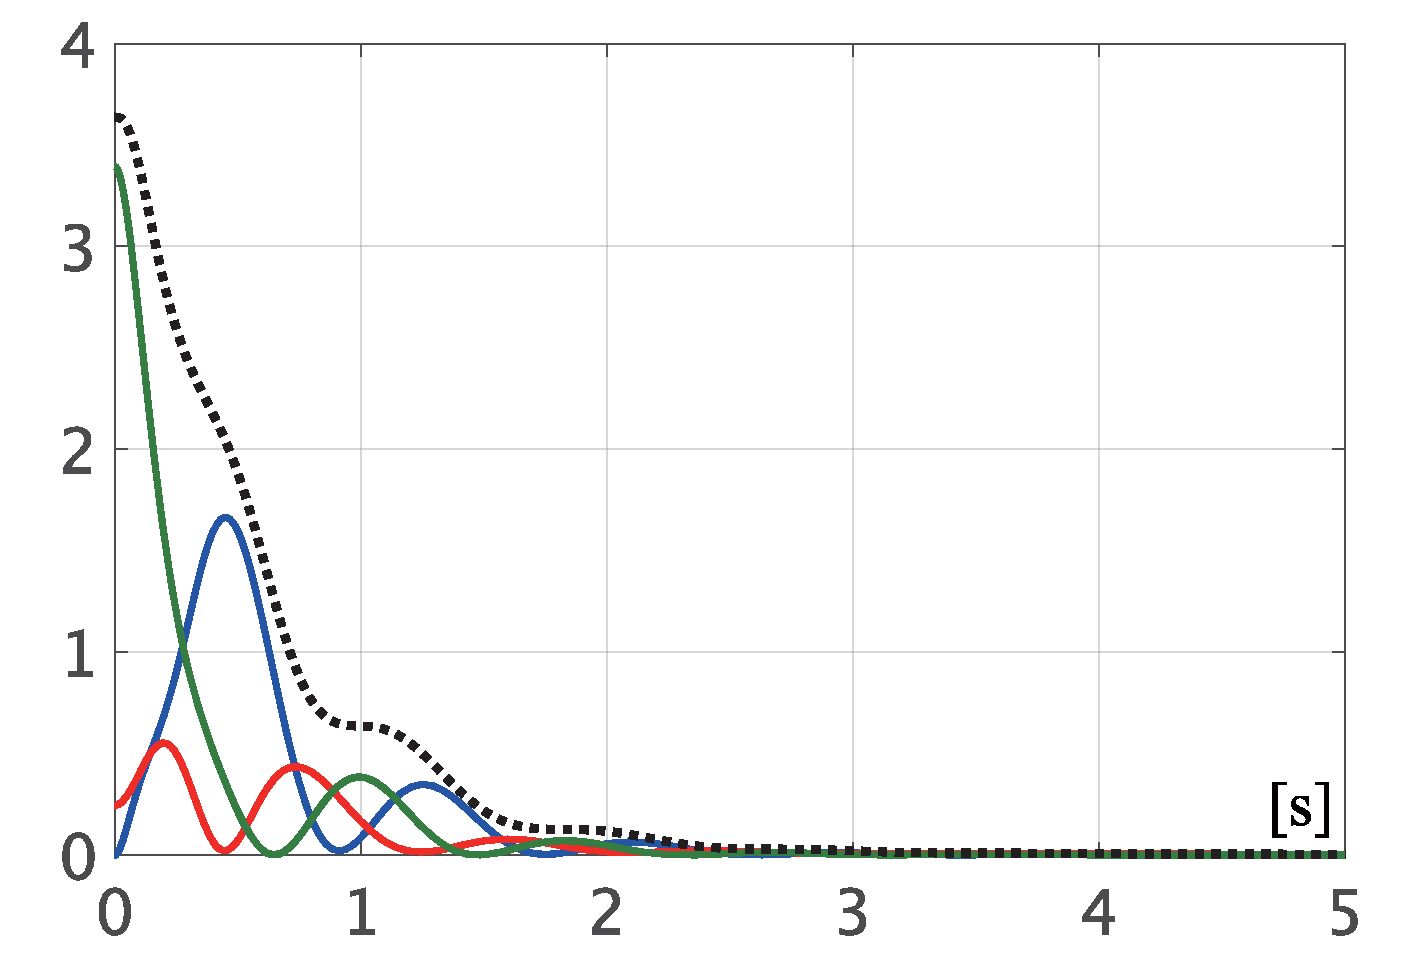
\includegraphics[width = 1.0\linewidth]{figs/Wnlin1}
    \subcaption{Initial values corresponding to steady-state condition 1}
%    \medskip
  \end{minipage}
  \begin{minipage}{0.49\linewidth}
    \centering
    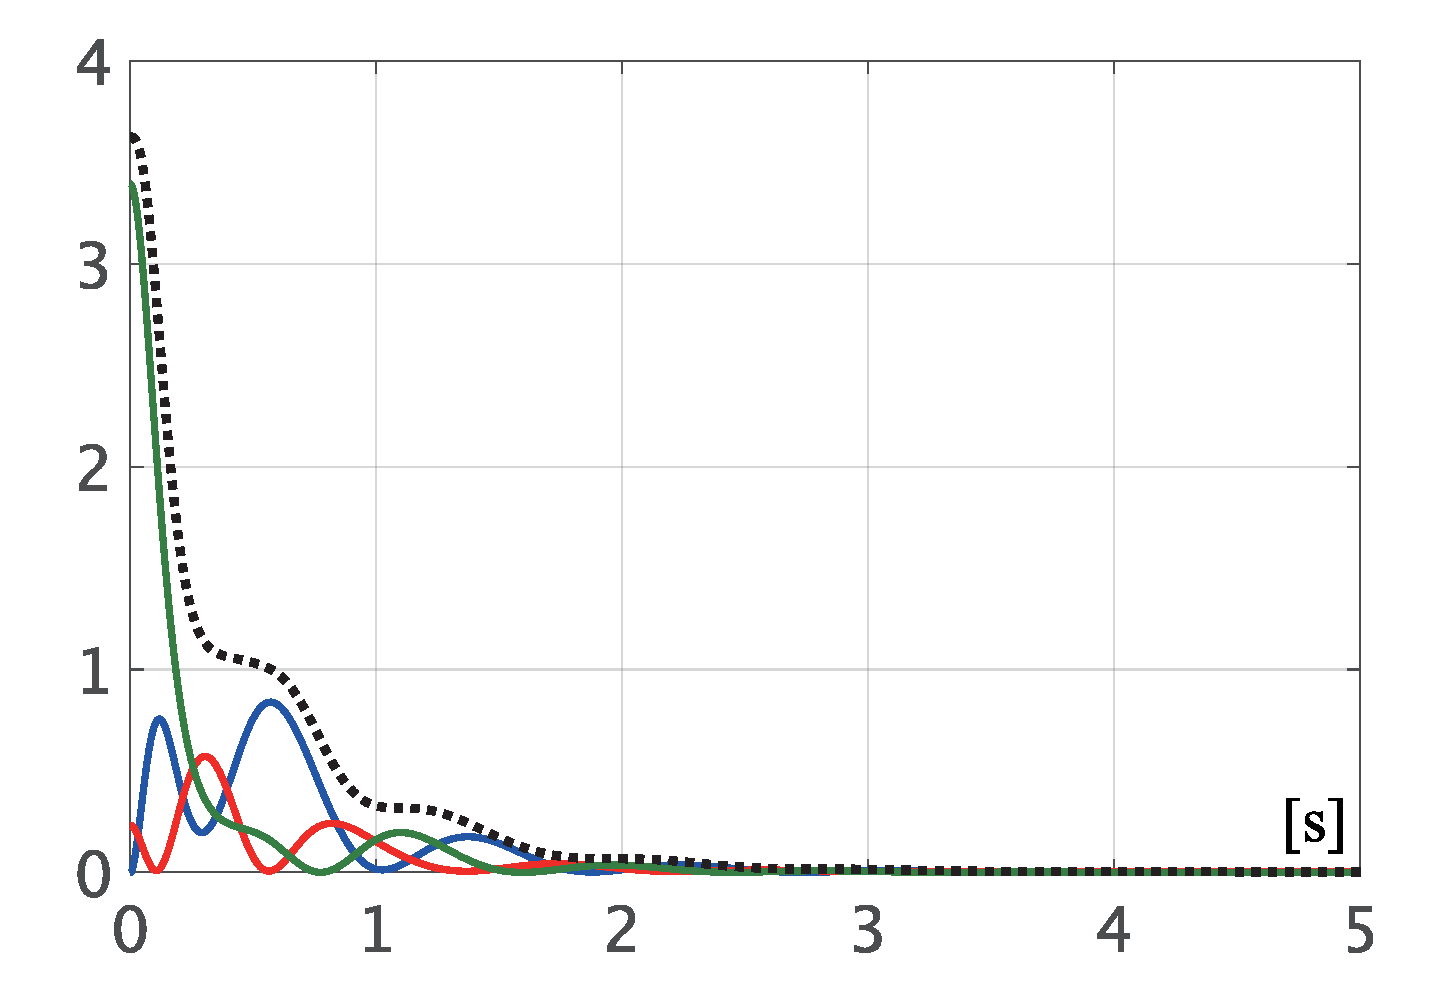
\includegraphics[width = 1.0\linewidth]{figs/Wnlin2}
    \subcaption{Initial values corresponding to steady-state condition 2}
%    \medskip
  \end{minipage}
  }
  \medskip
  \caption{\textbf{The time variation of the storage function for the initial value response}
  \\  \centering(Blue: $W_{x^{\star}_{\mathds{F}}}$, Red:$W_{x^{\star}_{\mathds{G}}}$,
  Green: $W_{\xi^{\star}}$, Black: Total sum)}
  \label{fig:LyapWnlin}
\medskip
\end{figure}

\smallskip
\subsubsection{The range where the potential energy function is convex}

In the following, we show that the conditions for the potential energy function
$U_{\mathds{G}}(x_{\mathds{G}})$ in Equation \ref{eq:potWx} to be a convex
function correspond to the passive power transmission conditions (i) and (iii)
discussed in Definition \ref{def:passtrans} in the analysis of the passive
properties of the linear approximation model. Note that assumption (ii) of the
passive power transmission conditions is assumed in this section.

We consider the case where generators are connected to all buses, in accordance
with the setting of the linear approximation model in Section
\ref{sec:linpasana}. That is, the subscripts for the generator buses and load
buses are

\[
  \mathcal{I}_{\rm G} = \{1,\ldots,N\}
  ,\qquad
  \mathcal{I}_{\rm L} = \emptyset
\]

In this case, applying the Kron reduction to the generator buses allows us to
obtain an equivalent system of ordinary differential equations for the
electrical subsystem $\mathds{G}$ in Equation \ref{eq:sys2G}, with respect to $i
\in \mathcal{I}_{\rm G}$, given by:

\begin{equation*}%\label{eq:kronGds}
  \mathds{G}_i : 
  \simode{
    \dot{\delta}_i &= u_{\mathds{G}_i}
    \\
    \taudi \dot{E}_i & = 
    -\tfrac{ \Xsi }{ \Xti }E_i
    - \left(
    \Xsi - \Xti
    \right)
    \sum_{j=1}^{N}
    E_j 
    B_{ij}^{\rm red}
    \sfcos \delta_{ij}
    + V_{{\rm field}i}^{\star}
    \\
    y_{\mathds{G}_i}&=  -E_i \sum_{j=1}^{N}
    E_j 
    B_{ij}^{\rm red}
    \sfsin \delta_{ij}
  }
\end{equation*}
where $\delta_{ij}$ denotes $\delta_i -\delta_j$. Also, the reduced susceptance
$B_{ij}^{\rm red}$ is defined as the $(i,j)$-th element of the matrix $B^{\rm
red}$, which is obtained by combining the susceptance matrix $B$ of the power
network in Eq. (\ref{eq:sys2G}), and is defined as follows:

\begin{equation}\label{eq:susred}
  B^{\rm red}
  := -
  \bigl\{
  \sfdiag \left( \Xti \right)   
  -
  \sfdiag \left( \Xti \right) B \sfdiag \left( \Xti \right)
  \bigr\}^{-1}
\end{equation}

The potential energy function corresponding to the representation of this system
of ordinary differential equations is given by Equation \ref{eq:potWx}. It is
expressed as follows in Equation \ref{eq:potWxred}:

\begin{equation}\label{eq:potWxred}
  U_{\mathds{G}}^{\rm red} (z_{\mathds{G}})  := 
  \frac{1}{2} 
  \sum_{i=1}^N
  \left\{
  \frac{ \Xsi E_i^2 }{ \Xti ( \Xsi - \Xti )}  
  + E_i \sum_{j=1}^{N}
  E_j 
  B_{ij}^{\rm red}
  \sfcos \delta_{ij}
  \right\}
\end{equation}
where the vector with all $\delta_i$ and $E_i$ is expressed as $z_{\mathds{G}}$.
If we calculate the partial differential related to the internal state, the
following is obtained:

\begin{equation*}
  \frac{\partial U_{\mathds{G}}^{\rm red} }{\partial \delta_i}(z_{\mathds{G}})  = y_{\mathds{G}_i}
  ,\qquad
  \frac{\partial U_{\mathds{G}}^{\rm red} }{\partial E_i} (z_{\mathds{G}}) = 
  \frac{V_{{\rm field}i}^{\star} - \taudi\dot{E}_i  }{ \Xsi - \Xti }
\end{equation*}

Similarly, for the steady state, we have:

\begin{equation*}
\frac{\partial U_{\mathds{G}}^{\rm red} }{\partial \delta_i} ( z^{\star}_{\mathds{G}} )
= y_{\mathds{G}_i}^{\star}
,\qquad
\frac{\partial U_{\mathds{G}}^{\rm red} }{\partial E_i} ( z^{\star}_{\mathds{G}} ) = 
\frac{V_{{\rm field}i}^{\star}  }{ \Xsi - \Xti }
\end{equation*}

Therefore, if we define the corresponding storage function as:

\[ 
  W_{z^{\star}_{\mathds{G}}}^{\rm red} (z_{\mathds{G}}) = U_{\mathds{G}}^{\rm red} (z_{\mathds{G}}) 
  - U_{\mathds{G}}^{\rm red} (z^{\star}_{\mathds{G}}) 
  - \left\{ \nabla U_{\mathds{G}}^{\rm red}(z^{\star}_{\mathds{G}}) \right\}^{\sf T}
  (z_{\mathds{G}}-z^{\star}_{\mathds{G}})
\]

Then, similarly to Equation \ref{eq:disineqGds}, its time derivative can be
bounded as:

\[
  \frac{d}{dt}W_{z^{\star}_{\mathds{G}}}^{\rm red} \bigl(z_{\mathds{G}}(t) \bigr)
  \leq 
  (y_{\mathds{G}}-y_{\mathds{G}}^{\star})^{\sf T} (u_{\mathds{G}}- u_{\mathds{G}}^{\star})
\]

Note that all elements of the reduced susceptance matrix $B^{\rm red}$ in
Equation \ref{eq:susred} are non-positive. This fact can be shown as follows.
From the discussion in the Section \ref{sec:admathp}, the susceptance matrix $B$
is a negative definite matrix with non-diagonal elements that are nonnegative.
Therefore:

\[
  B_{-}:= \sfdiag \left( \Xti \right)   
  -
  \sfdiag \left( \Xti \right) B \sfdiag \left( \Xti \right)
\]
is a positive definite matrix with non-positive off-diagonal elements, known as
an \textbf{M-matrix}\index{M-matrix}. It is known that all elements of the
inverse of an M-matrix are non-negative \cite{kodama1981system}. Therefore, all
elements of $B^{\rm red}=-B_-^{-1}$ are non-positive.

\begin{COLUMN}
\noindent \textbf{Hessian matrix}:
A condition necessary for a twice-differentiable function
$f:\mathbb{R}^n\rightarrow \mathbb{R}$ to be a convex over a certain range
$\mathcal{X}$ is that the following matrix is positive semi-definite for all
$x\in \mathcal{X}$:

\[
  \nabla^2 f(x):=
  \mat{
  \tfrac{\partial^2 f}{\partial x_1^2} (x) & \cdots & \tfrac{\partial^2 f}{\partial x_1 \partial x_n} (x) \\
  \vdots & \ddots & \vdots \\
  \tfrac{\partial^2 f}{\partial x_n \partial x_1} (x) & \cdots &\tfrac{\partial^2 f}{\partial x_n^2} (x)
  }
\]

This matrix is called the \textbf{Hessian matrix} of the function $f$
\cite{boyd2004convex}.
\end{COLUMN}

The convexity of the potential energy function $U_{\mathds{G}}^{\rm red}
(z_{\mathds{G}})$ in Equation \ref{eq:potWxred} is characterized by the positive
semidefiniteness of its Hessian matrix $\nabla^2 U_{\mathds{G}}^{\rm red}
(z_{\mathds{G}})$. Computing this Hessian matrix yields to:

\begin{equation}\label{eq:UGhess}
  \nabla^2 U_{\mathds{G}}^{\rm red} (z_{\mathds{G}})
  =
  \mat{
  L(z_{\mathds{G}})  &  - \hat{B}^{\sf T}(z_{\mathds{G}}) \\
  - \hat{B}(z_{\mathds{G}}) & -\hat{A}(z_{\mathds{G}})
  }
\end{equation}

However, the matrix constituting each block has the element $(i,j)$ given by:

\begin{equation*}
  \spliteq{
  L_{ij}(z_{\mathds{G}}) & := 
  \frac{\partial^2 U_{\mathds{G}}^{\rm red} }{\partial \delta_i \partial \delta_j} (z_{\mathds{G}})
  =
  \left\{
  \begin{array}{cl}
  -E_i \sum_{j=1, j\neq i}^{N} E_j B_{ij}^{\rm red} \sfcos(\delta_{ij}), &\quad i=j \\
  E_i  E_j B_{ij}^{\rm red} \sfcos(\delta_{ij}), & \quad i\neq j
  \end{array}
  \right.
    \\
  \hat{A}_{ij}(z_{\mathds{G}}) &:=  
  - \frac{\partial^2 U_{\mathds{G}}^{\rm red} }{\partial E_i \partial E_j} (z_{\mathds{G}})
  =
  \left\{
  \begin{array}{cl}
  -\left(B_{ii}^{\rm red}+\tfrac{ \Xsi }{ \Xti ( \Xsi - \Xti )} \right), &\quad i=j \\
  -B_{ij}^{\rm red} \sfcos(\delta_{ij}), & \quad i\neq j
  \end{array}
  \right. \\
  \hat{B}_{ij}(z_{\mathds{G}})  &:= 
  - \frac{\partial^2 U_{\mathds{G}}^{\rm red} }{\partial E_i \partial \delta_j} (z_{\mathds{G}})
  =
  \left\{
  \begin{array}{cl}
  \sum_{j=1, j\neq i}^{N} E_j B_{ij}^{\rm red} \sfsin(\delta_{ij}), &\quad i=j \\
  -E_j B_{ij}^{\rm red} \sfsin(\delta_{ij}), & \quad i\neq j
  \end{array}
  \right. 
  }
\end{equation*}

The Hessian matrix evaluated at the equilibrium point in Equation
\ref{eq:UGhess}, $\nabla^2 U_{\mathds{G}}^{\rm red} (z_{\mathds{G}}^{\star})$,
is identical to the matrix $P_G$ in Equation \ref{eq:defPG}, which appeared in
the passive analysis of the linearized electric subsystem in Section
\ref{sec:linpasana}. Note that the positive semi-definiteness of $P_G$
guarantees that the accumulation function for demonstrating the passivity of the
linearized model of $\mathds{G}$ is a positive semi-definite function.
Therefore, it is understood that the necessary and sufficient condition for
$U_{\mathds{G}}^{\rm red} (z_{\mathds{G}}^{\star})$ to be a convex function is
equivalent to the necessary and sufficient condition for $P_G$ to be positive
semi-definite, which is equivalent to the passive power transmission conditions
(i) and (iii) being satisfied.

In combination with the results from Section \ref{sec:linmathana}, it can be
understood that the region defined as the convex set of the potential energy
function $U_{\mathds{G}}^{\rm red} (z_{\mathds{G}})$ given in Equation
\ref{eq:potWxred}:

\[
  \mathcal{E}_{\mathds{G}}:=
  \left\{
  z_{\mathds{G}}^{\star} : \nabla^2 U_{\mathds{G}}^{\rm red} (z_{\mathds{G}}^{\star}) 
  \succeq 0
  \right\}
\]
is also the "maximum" set of equilibrium points that can demonstrate frequency
stability based on passivity.

The reason for this is that the passive power transmission conditions are
necessary conditions for the linearized electric subsystem to be passive in the
vicinity of a specific equilibrium point, as shown in Section
\ref{sec:nesconana}.  Therefore, for equilibrium points $z_{\mathds{G}}^{\star}$
where $\nabla^2 U_{\mathds{G}}^{\rm red} (z_{\mathds{G}}^{\star}) $ is not
positive semi-definite, the electric subsystem $\mathds{G}$ cannot be passive.

On the other hand, if the initial value of the electrical subsystem
$z_{\mathds{G}}(0)$ is set in the vicinity of a certain equilibrium point
$z_{\mathds{G}}^{\star}$ belonging to the set $\mathcal{E}_{\mathds{G}}$, then
for all combinations of physical parameters $(M_i, D_i, \taudi)_{i \in
\mathcal{I}_{\rm G}}$, the entire feedback control system will asymptotically
converge to a steady-state power flow state where demand and supply are
balanced.

For example, consider a situation where the power consumption of a certain load
changes in a stepwise and small manner from a steady-state power flow state
where demand and supply are balanced. In this case, since the equilibrium point
of the electrical subsystem $\mathds{G}$ undergoes a small variation from the
original steady-state power flow state to the new one, the initial time can be
regarded as the time when the power consumption changes and the initial value of
$\mathds{G}$ can be set in the vicinity of the equilibrium point.

From the above analytical result, it can be concluded that as long as the time
variation of model parameters such as loads and controller parameters is
sufficiently gradual and the power system state remains in the region where the
potential energy function becomes a convex function, frequency stability is
maintained by automatic generation control.

\section{Transient stability control}\label{sec:transcont}

\subsection{Decentralized control of generators with excitation system}

In power system engineering, the term \textbf{transient
stability}\index{transient stability} is widely used when discussing the size
and stability of the stability region of the equilibrium point. In this section,
we outline the mathematical models and characteristics of \textbf{excitation
systems}\index{excitation system} implemented for the purpose of increasing the
transient stability of the power system. Excitation systems are generally local
controllers implemented "individually" for each generator, which perform control
operations that automatically adjust the field input by locally measuring the
voltage phase or current phase of the bus to which the generator is connected,
as well as the internal state of the generator. The main element of an
excitation system is the \textbf{Automatic Voltage Regulator}
(AVR)\index{Automatic Voltage Regulator}, a control device that maintains the
bus voltage at the desired value. In addition, to suppress oscillations caused
by the AVR, additional control algorithms called \textbf{Power System
Stabilizers} (PSS)\index{Power System Stabilizer} may also be incorporated. In
Sections \ref{sec:avrov} to \ref{sec:pssov}, we will explain these standard
models and control effects.

\subsection{Standard Automatic Voltage Regulator model}\label{sec:avrov}

There are many standardized models for automatic voltage regulators. For
example, the IEEE's standardization report \cite{ieee2016ieee} lists more than
40 standard models. Automatic voltage regulator models are broadly classified
into direct current (DC), alternating current (AC), and static types. In the
following, we describe representative models of DC and static types.

First, we describe the \textbf{IEEE Type DC1 excitation system model}\index{IEEE
Type DC1 excitation system model}, which is a direct current (DC) model of the
automatic voltage regulator. For detailed modeling, please refer to
\cite[Section 7.9.2]{anderson2008power} or \cite[Section
8.6.3]{kundur1994power}. Here, we discuss the automatic voltage regulator for a
generator connected to bus $i$. To simplify the notation, we omit the subscript
$i$. Specifically, we use the generator model discussed in Section
\ref{sec:genfund}:

\begin{equation}\label{eq:gendifavr}
  \simode{
    \dot{\delta}&= \omega_0  \Delta \omega\\
    M   \Delta \dot{\omega}&= 
    - D \Delta\omega  
    - P
    +P_{{\rm mech}}
    \\
    \taud \dot{E} & = 
    - \Ifd 
    + V_{{\rm field}}
  }
\end{equation}

However, for the sake of the following discussion, we define the value of the
excitation current of the generator in the units of pu as:

\begin{equation}\label{eq:efield}
  \Ifd := \frac{ \Xs }{ \Xt }E
  -\left(
  \frac{ \Xs }{ \Xt }-1
  \right)
  |\bm{V}| \sfcos (\delta - \angle \bm{V} )
\end{equation}

The active and reactive powers output by the generator are given by:

\[
  P  =  \frac{E |\bm{V} |}{ \Xt } \sfsin(\delta -  \angle \bm{V}), \qquad
  Q  =  \frac{E |\bm{V} |}{ \Xt } \sfcos (\delta - \angle \bm{V}) - \frac{|\bm{V}|^2}{ \Xt }
\]

It should be noted that for the salient-pole generator model discussed in
section \ref{sec:genmodadv}, we replace $\Xt$ and $\Xs$ in Equation
\ref{eq:efield} with $X_{{\rm d}}'$ and $X_{\rm d}$, respectively, to define
$\Ifd$.

As shown in Figure \ref{fig:avrdc1}, the IEEE DC1 model of the automatic voltage
regulator is a controller that takes the magnitude $|\bm{V}|$ of the bus voltage
phasor as input and outputs the field excitation input $V_{\rm field}$ of the
generator. However, as additional input signals, a reference signal $V_{\rm
ref}^{\star}$ for adjusting the magnitude of the bus voltage phasor to the
desired value and a control signal $V_{\rm pss}$ output by the power system
stabilizer are applied. The IEEE DC1 model of the automatic voltage regulator
consists of four basic devices: a voltage transformer, a comparator, an
amplifier, and an exciter, as well as an auxiliary stabilizing circuit. In the
following, we will explain the dynamic characteristics of each device.

\begin{figure}[t]
  \centering
  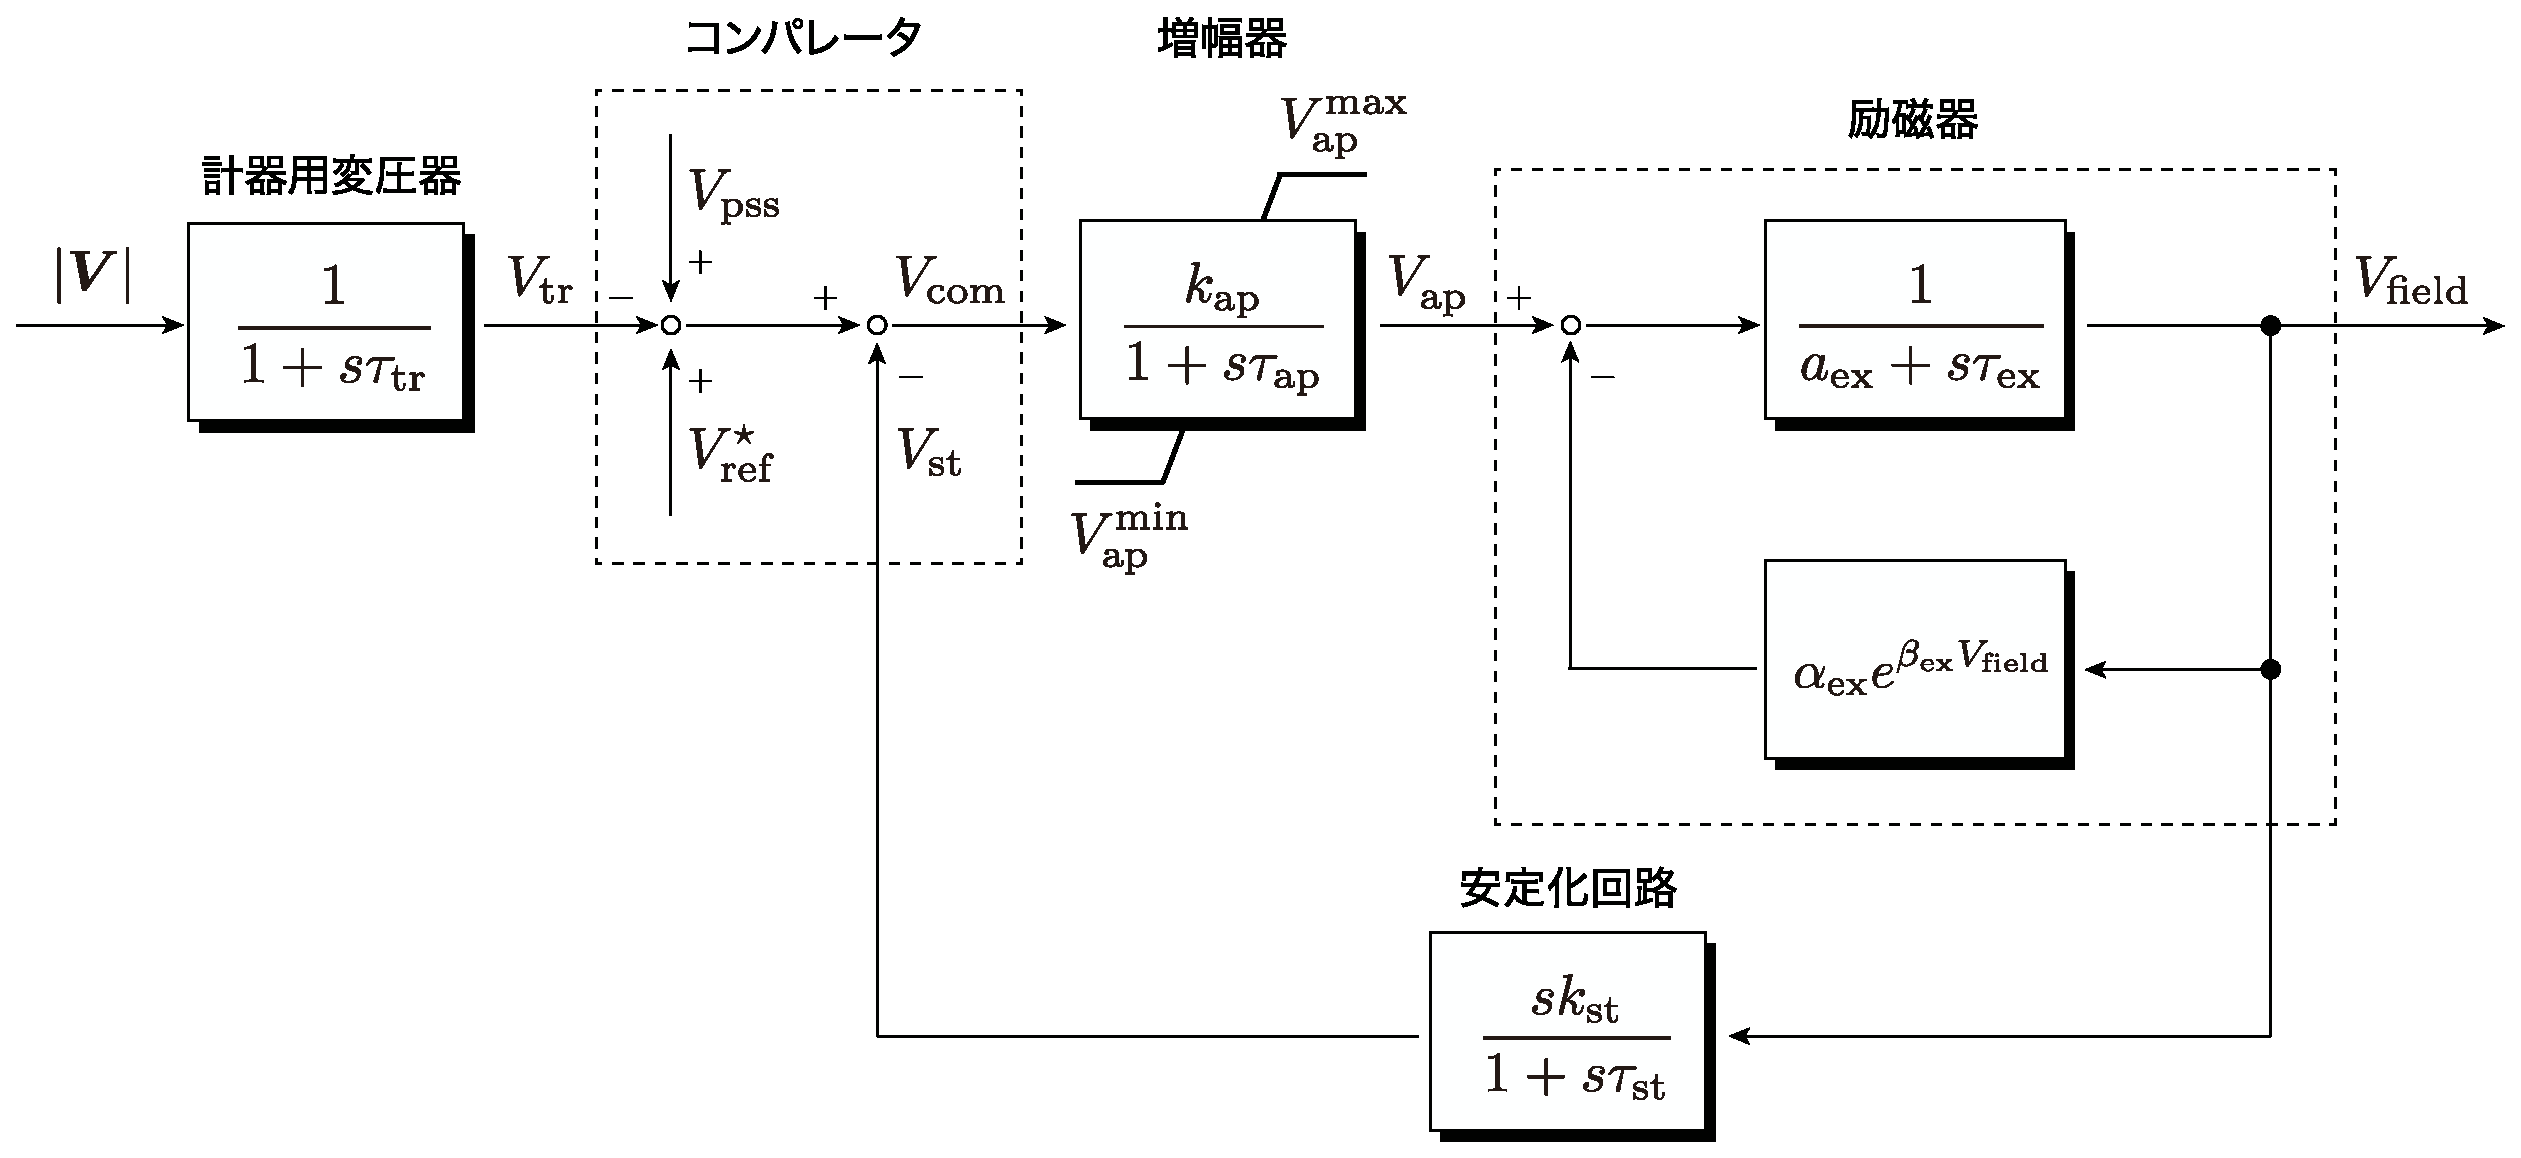
\includegraphics[width = 0.99\linewidth]{figs/avrdc1}
  \medskip
  \caption{\textbf{IEEE DC1 type model of automatic voltage regulator}}
  \label{fig:avrdc1}
  \medskip
\end{figure}

\smallskip
\subsubsection{Voltage transformer}

\begin{subequations}\label{eq:stanAVR}
The voltage transformer is a device that reduces the bus voltage to a voltage
that can be used by the control circuit, and its dynamic characteristics is
modeled as a first-order lag filter:

\begin{equation}\label{eq:trnsmod}
  \tau_{\rm tr} \dot{V}_{\rm tr} = - V_{\rm tr} +  |\bm{V}|
\end{equation}

Generally, the time constant $\tau_{\rm tr}$ is sufficiently small, and the
output $V_{\rm tr}$ of the voltage transformer is almost equal to the
absolute value of the bus voltage $|\bm{V}|$.

\smallskip
\subsubsection{Comparator}

The comparator is a device that outputs the difference between the output
$V_{\rm tr}$ of the voltage transformer and the reference signal $V_{\rm
ref}^{\star}$. The output $V_{\rm pss}$ of the power system stabilizer mentioned
later is applied as a signal to adjust the constant $V_{\rm ref}^{\star}$. In
addition, when incorporating a stabilizing circuit for the excitation system,
its output $V_{\rm st}$ is also fed back. That is, the comparator is modeled as

\begin{equation}\label{eq:compmod}
  V_{\rm com} = V_{\rm ref}^{\star} + V_{\rm pss}- V_{\rm tr}
  - V_{\rm st}
\end{equation}

As mentioned above, since $V_{\rm tr}$ is almost equal to $|\bm{V}|$ because the
time constant $\tau_{\rm tr}$ is usually very small, if the output $V_{\rm pss}$
of the power system stabilizer and the output $V_{\rm st}$ of the stabilizing
circuit are zero, the output $V_{\rm com}$ of the comparator is almost equal to
the difference between the reference signal and the absolute value of the bus
voltage phase $V_{\rm ref}^{\star} - |\bm{V}|$.

\smallskip
\subsubsection{Amplifier}

The amplifier is a device that amplifies the output $V_{\rm com}$ of the
comparator to drive the excitation system. There are various types, such as
rotary and electromagnetic types, but in many cases, it is modeled as:

\begin{equation}\label{eq:ampmod}
  \tau_{\rm ap} \dot{V}_{\rm ap}=
  \left\{
  \begin{array}{cl}
  - V_{\rm ap} + k_{\rm ap} V_{\rm com}, & \mbox{$V_{\rm ap}^{\rm min} < V_{\rm ap} < V_{\rm ap}^{\rm max}$ ~or~ $V_{\rm ap} V_{\rm com}\leq 0$ } \\
  0, & \mbox{otherwise}
  \end{array}
  \right.
\end{equation}
where the time constant $\tau_{\rm ap}$ and gain $k_{\rm ap}$ are non-negative
constants, and the saturation that constrains the internal state $V_{\rm ap}$ to
the range $[V_{\rm ap}^{\rm min},V_{\rm ap}^{\rm max}]$ is expressed by the
conditional branching. Note that in some cases, saturation is applied to the
output instead of the internal state, and in transient states with large
disturbances such as ground faults, the width of the saturation limits may be
set large \cite[Section 4.3]{sauer2017power}.

\smallskip
\subsubsection{Exciter}
The exciter is a device that generates the field input $V_{\rm field}$ from the
output $V_{\rm ap}^{\rm sat}$ of the amplifier, modeled as a nonlinear
first-order system given by:

\begin{equation}\label{eq:extmod}
  \tau_{\rm ex}\dot{V}_{\rm field} =
  - \Bigl( 
  a_{\rm ex} + 
  \underbrace{\alpha_{\rm ex} e^{\beta_{\rm ex} V_{\rm field}}}_{\ast} 
  \Bigr) V_{\rm field}
  +V_{\rm ap}
\end{equation}

Here, $\tau_{\rm ex}$ is a positive constant, but the sign of $a_{\rm ex}$ may
vary depending on the literature. The term denoted by "$\ast$" represents the
nonlinearity due to magnetic saturation and other effects within the exciter,
and $\alpha_{\rm ex}$ and $\beta_{\rm ex}$ are both non-negative constants.
These constants are typically set to ensure stable dynamic behavior of the
exciter in the vicinity of the normal operating point.

\smallskip
\subsubsection{Stabilizing circuit}
The stabilizing circuit is a circuit that is implemented to enhance the
stability of the excitation system. In the IEEE DC1 model, it is represented as
a mechanism that feeds back the differential value of the field input. That is,
its dynamic characteristics are expressed as:

\begin{equation}\label{eq:stcmod}
  \tau_{\rm st}\dot{V}_{\rm st} =
  - V_{\rm st}
  + k_{\rm st} \dot{V}_{\rm field}
\end{equation}
where the time constant $\tau_{\rm st}$ and gain $k_{\rm st}$ are non-negative
constants. The output $V_{\rm st}$ of this stabilization circuit is fed back to
the comparator in Equation \ref{eq:compmod}.

\end{subequations}

The IEEE Type DC1 excitation system model of AVR is a combination of Equation
\ref{eq:trnsmod} to Equation \ref{eq:stcmod} discussed above. The reference
values of each parameter are summarized in \ref{table:AVRpara1} and
\ref{table:AVRpara2}. The unit of the time constant is [s] while other units are
[pu].

\begin{table}[ht]
\medskip
 \caption{\textbf{Parameter example of IEEE DC1 type model}}
 \label{table:AVRpara1}
 \centering
  \begin{tabular}{lcccccc}
   \hline
 &  $\tau_{\rm tr}$ & $\tau_{\rm ap}$ & $k_{\rm ap}$ & $V_{\rm ap}^{\rm max}$ & $V_{\rm ap}^{\rm min}$ \\
   \hline \hline
   Example 1 \cite[Table D.3. Unit F2]{anderson2008power}& 0.00 & 0.05 & 57.1 & 1.00 & $-1.00$\\
   Exapmle 2 \cite[Table 7.3]{sauer2017power}& 0.00 & 0.2 & 20 & $\infty$ & $-\infty$\\
   \hline
  \end{tabular}
\end{table}

\begin{table}[ht]
\medskip
 \caption{\textbf{Parameter example of IEEE DC1 type model (continued)}}
 \label{table:AVRpara2}
 \centering
  \begin{tabular}{lccccccc}
   \hline
&    $\tau_{\rm ex}$ & $a_{\rm ex}$ & $\alpha_{\rm ex}$ & $\beta_{\rm ex}$ & $\tau_{\rm st}$ & $k_{\rm st}$\\
   \hline \hline
   Example 1 \cite[Table D.3. Unit F2]{anderson2008power}& 0.50 & $-0.045$ & 0.0012 & 1.21 & 1.00 & 0.08\\
   Example 2 \cite[Table 7.3]{sauer2017power}& 0.314 & $1.0$ & 0.0039 & 1.555 & 0.35 & 0.063 \\
   \hline 
  \end{tabular}
\end{table}

\begin{figure}[t]
\centering
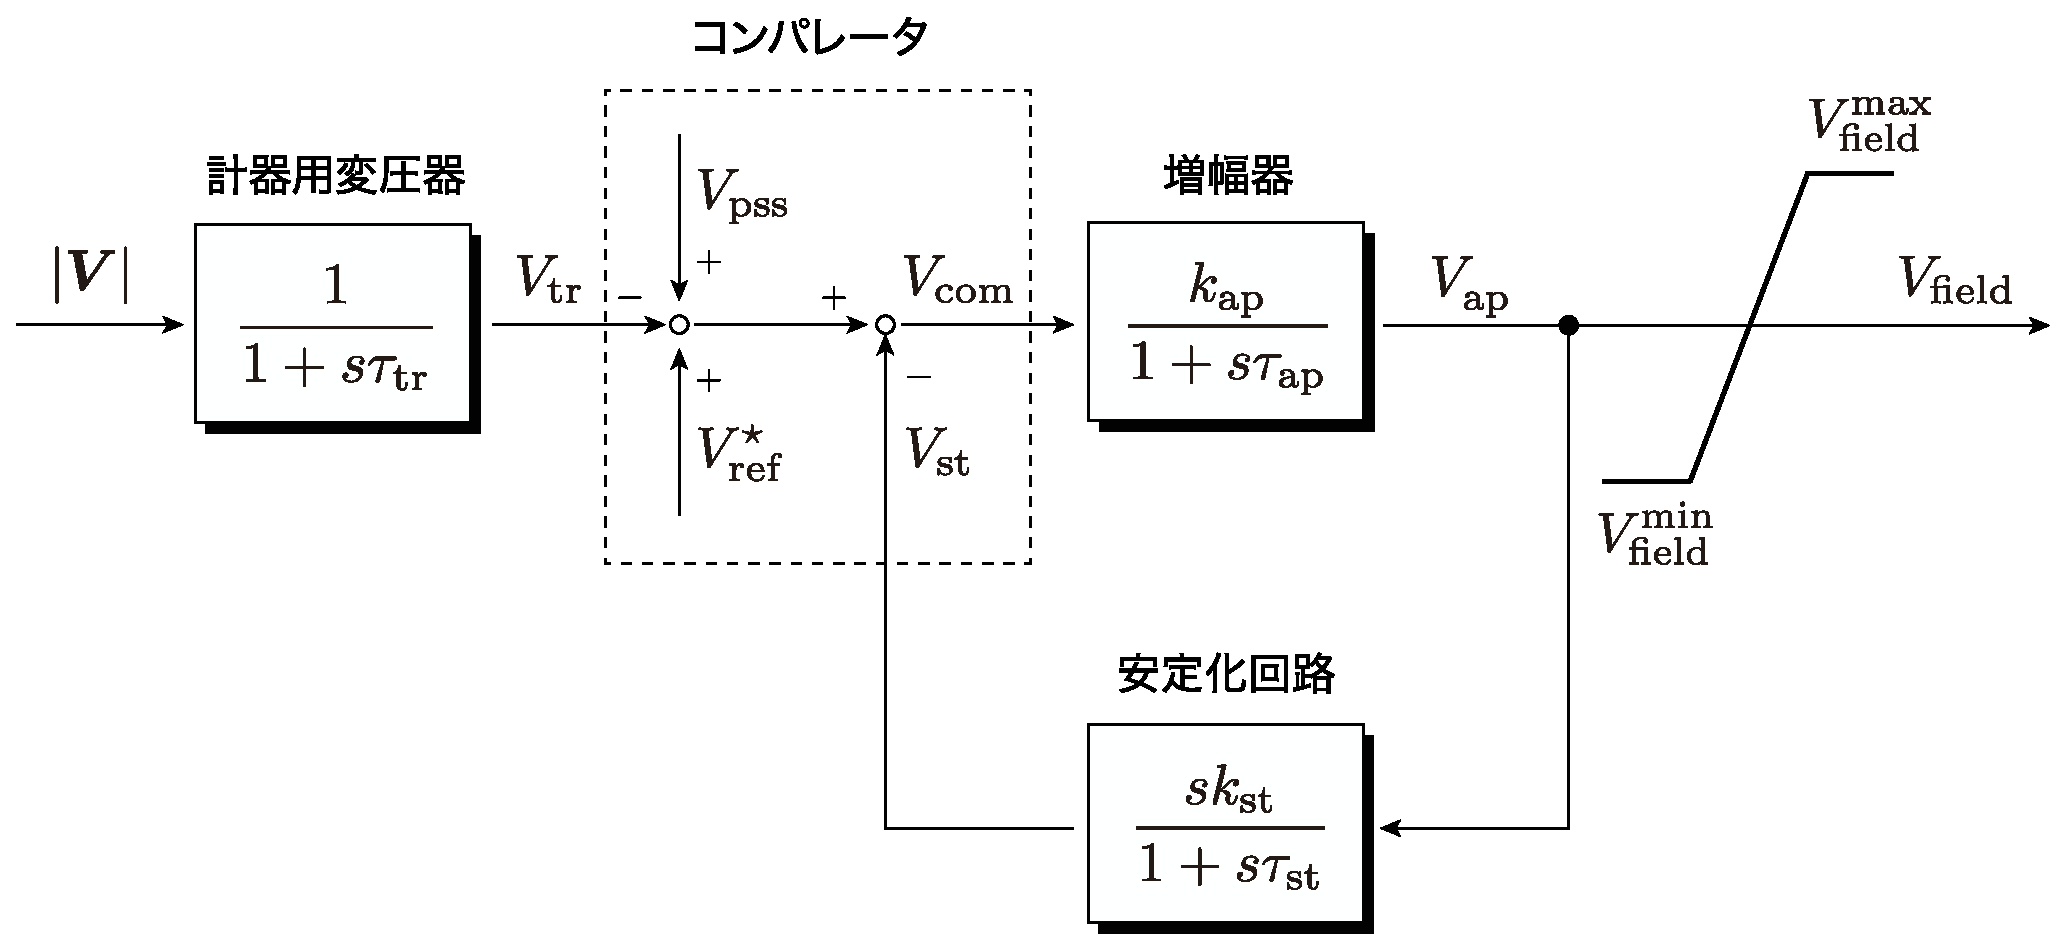
\includegraphics[width = .85\linewidth]{figs/avrst1}
\medskip
\caption{\textbf{IEEE ST1 type model of automatic voltage regulator}}
\label{fig:avrst1}
\medskip
\end{figure}

Next, we will explain the \textbf{IEEE Type ST1 excitation system model} which
has a similar structure to the IEEE DC1 type but is a static model with faster
response. In this automatic voltage regulator model, the excitation system time
constant is sufficiently small, and the excitation system model in Equation
\ref{eq:extmod} is expressed as a static relationship:

\[
  V_{\rm field} = \sfsat \bigl( V_{\rm ap};V_{\rm field}^{\rm min},V_{\rm field}^{\rm max} \bigr)
\]
where $\sfsat$ is the output saturation function defined by:

\[
  \sfsat(x;\underline{\alpha},\overline{\alpha}) := \left\{
  \begin{array}{cl}
  \underline{\alpha}, & x \leq \underline{\alpha} \\
  x, & \underline{\alpha} < x \leq \overline{\alpha} \\
  \overline{\alpha}, & x> \overline{\alpha}
  \end{array}
  \right.
\]

Additionally, the upper and lower limits of output saturation are modeled to
mainly depend on the absolute value of the bus voltage phase angle \cite[Section
8.63]{kundur1994power}. Specifically, using $|\bm{V}|$ and $\Ifd$ in Equation
\ref{eq:gendifavr}, they are given by

\[
  V_{\rm field}^{\rm min} = \gamma_{-} |\bm{V}|, \qquad
  V_{\rm field}^{\rm max} = \gamma_{+} |\bm{V}|
  -
  k_0 \Ifd
\]
where $\gamma_{-}$, $\gamma_{+}$, and $k_{0}$ are non-negative constants. The
block diagram of this model is shown in Figure \ref{fig:avrst1}. Note that during
a ground fault on the bus, $|\bm{V}|$ becomes 0, and the excitation input
$V_{\rm field}$ is not outputted from the AVR.

Since the excitation response of the IEEE ST1 model is fast enough, stabilizing
circuits are often unnecessary. When the amplifier time constant $\tau_{\rm ap}$
is small enough that its dynamic characteristics can be ignored, a simplified
first-order model given by Equation \ref{eq:avrst1} is used. For example, this
model is used in \cite[Section 12.4]{kundur1994power} and \cite[Section
4.2.2]{pal2006robust}. Examples of parameters are shown in Examples 1 and 2 of
Table \ref{table:AVRparast1}.

\begin{equation}\label{eq:avrst1}
  \simode{
    \tau_{\rm tr} \dot{V}_{\rm tr} & = - V_{\rm tr} +  |\bm{V}|  \\
    V_{\rm ap} &= k_{\rm ap} ( V_{\rm ref}^{\star} + V_{\rm pss}- V_{\rm tr} )\\
    V_{\rm field} & = \sfsat \left(
    V_{\rm ap};
    V_{\rm field}^{\rm min},V_{\rm field}^{\rm max} 
    \right)
  }
\end{equation}

\begin{table}[ht]
\medskip
 \caption{\textbf{IEEE ST1 type model parameter example}}
 \label{table:AVRparast1}
 \centering
  \begin{tabular}{lccccccccc}
   \hline
 &  $\tau_{\rm tr}$ & $\tau_{\rm ap}$ & $k_{\rm ap}$ & $\gamma_{+}$ & $\gamma_{-}$ & $k_{0}$ & $\tau_{\rm st}$ & $k_{\rm st}$\\
   \hline \hline
   Example 1 \cite[Section 8.6.3]{kundur1994power}& 0.015 & 0 & 200 & 7.00 & $-6.40$ & 0.04 & 0 & 0\\
   Example 2 \cite[Table H.23]{ieee2016ieee}& 0.02 & 0 & 210 & 6.43 & $-6.00$ & 0.038 & 0 & 0 \\
   Example 3 \cite[Section V]{chow2004power}& 0 & 0.076 & 36.66 & $\infty$ & $-\infty$ & 0 & 0 & 0 \\
   Example 4 \cite[Table 4]{sadamoto2019dynamic}& 0 & 0.05 & 20 & $\infty$ & $-\infty$ & 0 & 0 & 0 \\
   \hline
  \end{tabular}
\end{table}

When the time constant of the amplifier $\tau_{\rm ap}$ is not zero, but the
time constant of the instrument transformer $\tau_{\rm tr}$ is zero or a model
that excludes output saturation is often used
\cite{chow2004power,sauer2017power,sadamoto2019dynamic}, the following equation
can be used:

\begin{equation}\label{eq:avrst1s}
  \simode{
    \tau_{\rm ap} \dot{V}_{\rm ap}&=
    - V_{\rm ap} + k_{\rm ap} (V_{\rm ref}^{\star} + V_{\rm pss}- |\bm{V}|)\\
    {V}_{\rm field}&=V_{\rm ap}
  }
\end{equation}

Parameter examples of this model are shown in Example 3 and Example 4 of Table
\ref{table:AVRparast1}.

Note that when the desired steady-state value of the excitation input $V_{{\rm
field}}^{\star}$ and the absolute value of the bus voltage
$\left|\bm{V}^{\star}\right|$ are given, the reference signal $V_{{\rm
ref}}^{\star}$ for the reference is determined as follows:

\begin{equation}\label{eq:avrref}
  V_{{\rm ref}}^{\star} = \frac{V_{{\rm field}}^{\star}}{k_{{\rm ap}}}+|\bm{V}^{\star}|
\end{equation}

However, in actual power system operation, the steady-state values of bus
voltage and excitation input are unknown and can vary due to load distribution,
and other factors, so the value of the reference signal $V_{{\rm ref}}^{\star}$
is specified using standard values for bus voltage and excitation input.

\subsection{Control effectiveness of AVR}

Let's analyze the control effectiveness of the Automatic Voltage Regulator (AVR)
using a simple power system model.

\begin{example}{Effect of automatic voltage regulator on steady-state and
transient stability}\label{ex:avreffect}

Consider the three-bus power system model discussed in Examples \ref{ex:derY},
\ref{ex:pf3bus}, and \ref{ex:inires}. The physical constants of the generator
and transmission lines are set to the same values as in Example \ref{ex:inires}.
Furthermore, the load connected to bus 2 is modeled as a constant impedance, and
the impedance value is set to the first row of Table \ref{table:loadpara1}.  The
automatic voltage regulator is set to the IEEE ST1 type model in Equation
\ref{eq:avrst1}. The automatic voltage regulator incorporated in generators 1
and 3 is identical, and the parameter values are those of Example 1 in Table
\ref{table:AVRparast1}.

First, let us examine the change in the set of steady-state stable equilibrium
points due to the presence or absence of the automatic voltage regulator.
Specifically, the steady-state stability of the corresponding power system is
determined based on the approximate linearization by varying the difference in
steady-state values of the rotor angle, $\delta_3^{\star}-\delta_1^{\star}$,
while fixing the steady-state values of the internal voltage of the generators,
$E_1^{\star}$ and $E_3^{\star}$, to the values in the rightmost column of Table
\ref{table:genst13a}. By calculating the range of
$\delta_3^{\star}-\delta_1^{\star}$ where the approximate linear model is
stable, it is found that without the automatic voltage regulator, the range is
as shown in (i) of Table \ref{table:stableeqs}, while with the automatic voltage
regulator, the range is as shown in (ii) of Table \ref{table:stableeqs}.  From
this result, it is understood that the set of stable equilibrium points tends to
decrease due to the automatic voltage regulator.

Note that without loss of generality, $\delta_1^{\star}$ or $\delta_3^{\star}$
can be set to zero.  In addition, if the steady-state values of the internal
states of each generator are determined, the corresponding steady-state values
of the mechanical and field inputs can be determined by

\begin{equation*}
  \simode{
    P_{{\rm mech}i}^{\star} &= %\textstyle
      f_i \left( \delta^{\star},E^{\star} \right)
    \\
    V_{{\rm field}i}^{\star} & = %\textstyle
      \tfrac{ \Xsi }{\Xti }  E_i^{\star}  - \left(
    \Xsi - \Xti
    \right)
    g_i \left( \delta^{\star},E^{\star} \right)
  }
  \qquad
  i \in \{1,3\}
\end{equation*}
where $\delta^{\star}$ and $E^{\star}$ are vectors with $\delta_i^{\star}$ and
$E_i^{\star}$, and functions $f_i$ and $g_i$ are defined by Equation
\ref{eq:figidef}.

Furthermore, the steady-state value of the voltage phase of the generator bus
can be obtained using Equation \ref{eq:colVi} as follows:

\begin{equation*}
  \mat{
    \bm{V}_1^{\star}\\
    \bm{V}_3^{\star}
  } =
  \left(
    \mat{
    \tfrac{1}{\bm{j} \Xt_1 } & 0\\
    0 & \tfrac{1}{\bm{j} \Xt_3 }
    } + 
    \bm{Y}_{\rm Kron}
  \right)^{-1}
  \mat{
    \tfrac{e^{\bm{j} \delta_1^{\star}}}{\bm{j} \Xt_1 } & 0 \\
    0 & \tfrac{e^{\bm{j} \delta_3^{\star}}}{\bm{j} \Xt_3 }
  }
  \mat{
    E_1^{\star}  \\
    E_3^{\star} 
  }
\end{equation*}

Here, $\bm{Y}{\rm Kron}$ is the admittance matrix obtained by Kron reduction of
the load bus defined in equation \ref{eq:Kron}. The value of the reference
signal $V_{{\rm ref}i}^{\star}$ is determined by equation \ref{eq:avrref}.

\begin{table}[ht]
\medskip
 \caption{\textbf{Steady value of rotor declination that stabilizes the state} 
 \\ \centering(AVR: automatic voltage regulator, PSS: system stabilizer)}
 \label{table:stableeqs}
 \centering
  \begin{tabular}{ccccccccccc}
   \hline
 & (i) Without AVR & (ii) With AVR & (iii) With AVR and PSS \\
   \hline \hline
 $\delta_3^{\star}-\delta_1^{\star}$ Upper limit~[rad]  & $1.03$ & $0.87$ & $1.32$ \\
 $\delta_3^{\star}-\delta_1^{\star}$ Lower limit~[rad] & $-0.90$ & $-0.30$ & $-1.10$  \\
   \hline
  \end{tabular}
\end{table}

\begin{COLUMN}
\noindent \textbf{$\mathcal{L}_2$ norm}:
The \textbf{$\mathcal{L}_2$ norm}\index{L2 norm@$\mathcal{L}_2$ norm} of a
function $y:[0,\infty) \rightarrow \mathbb{R}^n$ is defined as

\[
  \|y\|_{\mathcal{L}_2} := \sqrt{
  \int^{\infty}_{0}
  \| y(\tau)\|^2  d \tau
}
\]

This value can be interpreted as the energy of a time-varying signal. Unless the
signal's amplitude decays over time, the $\mathcal{L}_2$ norm will generally be
infinite. The letter "$\mathcal{L}$" comes from the name of Henri Lebesgue, who is known for
his work on the theory of Lebesgue integration.
\end{COLUMN}

Next, let us confirm the improvement of transient stability by the automatic
voltage regulator. Specifically, we will conduct the following analysis. First,
regardless of the presence of the automatic voltage regulator, we consider a
steady-state stability with a steady-state value of the rotor angle difference
$\delta_3^{\star}-\delta_1^{\star}$ equal to $-\tfrac{\pi}{6}$~[rad]. The
steady-state value of the internal voltage is set to the above value. Next, we
change the initial values of the power system model as parameters and calculate
$\|\Delta\omega\|_{\mathcal{L}_2}$ for the time response of the obtained angular
frequency deviation. Here, $\Delta \omega$ is a vector consisting of $\Delta
\omega_1$ and $\Delta \omega_3$. Similarly, we calculate
$||\bm{V}|-|\bm{V}^{\star}||{\mathcal{L}_2}$ for the time response of the main
bus voltage phase deviation. Here, $|\bm{V}|$ is a vector consisting of
$\||\bm{V}|-|\bm{V}^{\star}| \|_{\mathcal{L}_2}$ is a vector consisting of
$|\bm{V}_1^{\star}|$ and $|\bm{V}_3^{\star}|$. Note that when the initial value
is given inside the stable region of the equilibrium point of interest, the
$\mathcal{L}_2$ norm values of the angular frequency deviation and the main bus
voltage phase deviation are finite. Moreover, it is known that the higher the
$\mathcal{L}_2$ norm values of these quantities, the higher the transient
stability of the equilibrium point for the given initial values. On the other
hand, when the initial value is given outside the stable region, the
$\mathcal{L}_2$ norm values become infinite.

The analysis results of the transient stability are shown in
Figure \ref{fig:transientL2}. The horizontal axis represents the initial value of
$\delta_3-\delta_1$ set, and the vertical axis represents the $\mathcal{L}_2$
norm value of the angular frequency deviation and the main bus voltage phase
deviation generated for the set initial value. The case without the automatic
voltage regulator corresponding to (i) in Table \ref{table:stableeqs} is
represented by a solid blue line, and the case with the automatic voltage
regulator corresponding to (ii) is represented by a dashed black line. Note that
the plots are shown for the range of initial values for which the
$\mathcal{L}_2$ norm values are finite. The initial values of the internal
voltage $E_1$ and $E_3$ are set to the same value as their steady-state value
$E_1^{\star}$ and $E_3^{\star}$, respectively. The initial values of the angular
frequency deviation $\Delta \omega_1$ and $\Delta \omega_3$ are both set to 0.
From this result, it can be seen that the transient stability of the angular
frequency deviation and the main bus voltage phase deviation has improved by
incorporating the automatic voltage regulator. It can also be seen that the

As a reference, the time response of the angular frequency deviation that occurs
when the initial value of $\delta_3-\delta_1$ is set to $-1$ and
$-\frac{\pi}{2}$, respectively, is shown in Figures \ref{fig:avrsmalld} and
\ref{fig:avrlarged}. (a) represents the case without automatic voltage regulator
and (b) represents the case with automatic voltage regulator. From these
results, it can be seen that incorporating an automatic voltage regulator tends
to make the low-frequency component (the center value) of the oscillation of the
angular frequency deviation converge to 0 more quickly. On the other hand, it is
also found that there is no significant change in the decay rate of the
high-frequency component of the oscillation, regardless of the presence or
absence of the automatic voltage regulator.
\end{example}

\begin{figure}[t]
  \centering
  {
  \begin{minipage}{0.49\linewidth}
    \centering
    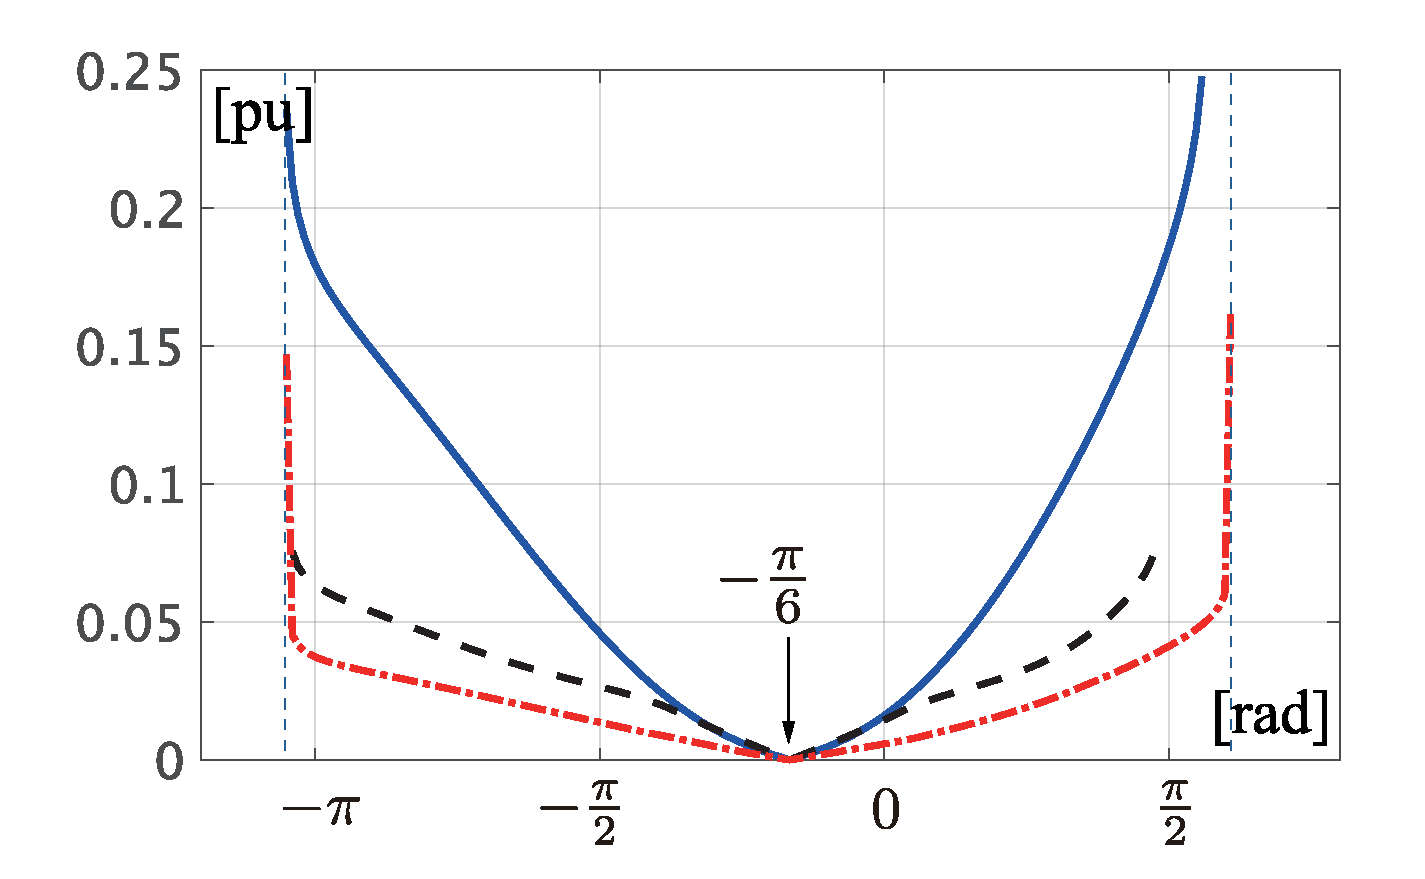
\includegraphics[width = 1.0\linewidth]{figs/transientL2w}
    \subcaption{ $\|\Delta\omega\|_{\mathcal{L}_2}$ }
  \end{minipage}
  \begin{minipage}{0.49\linewidth}
    \centering
    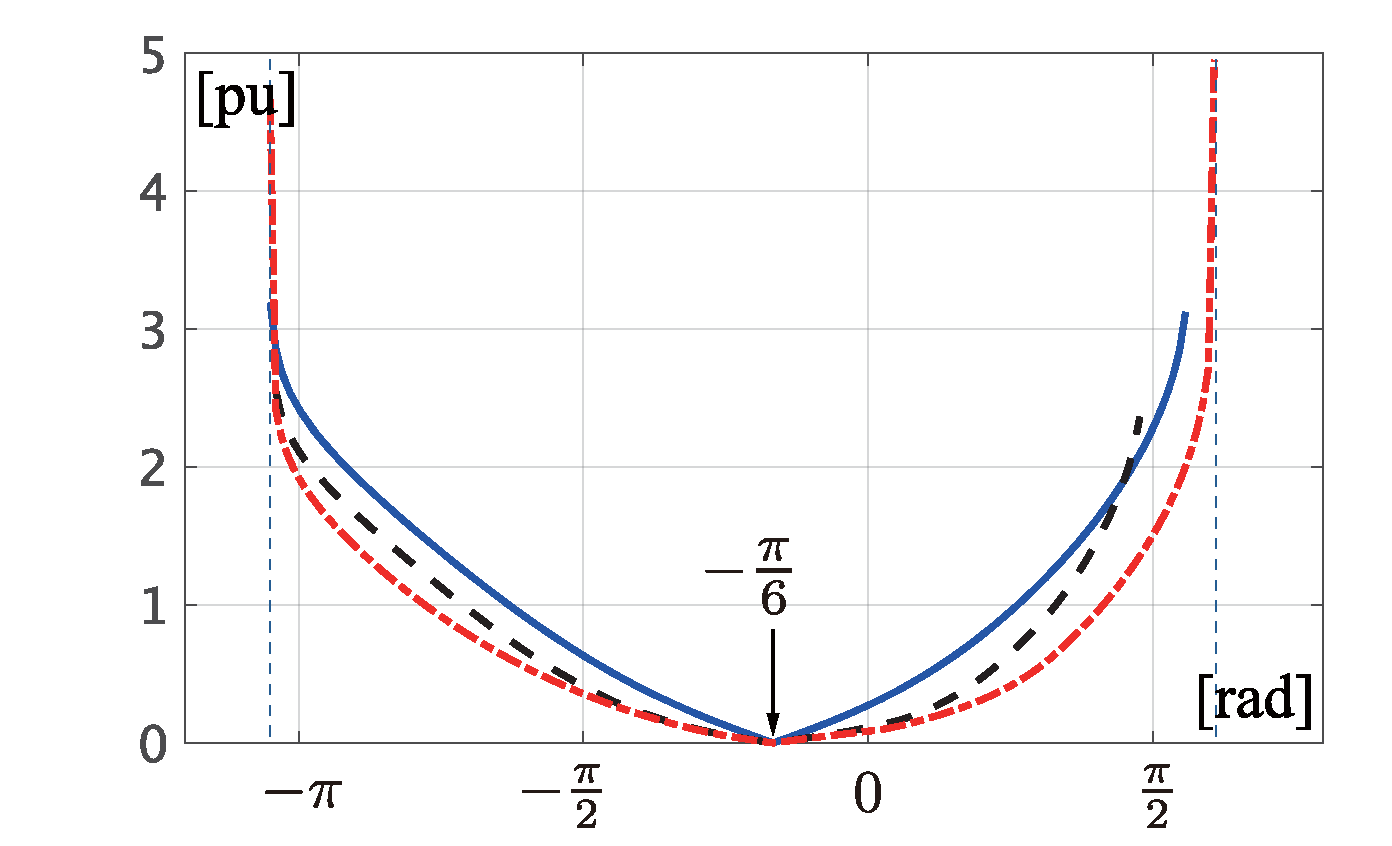
\includegraphics[width = 1.0\linewidth]{figs/transientL2V}
    \subcaption{ $\bigl\||\bm{V}|-|\bm{V}^{\star}| \bigr\|_{\mathcal{L}_2}$}
  \end{minipage}
  \medskip
  \caption{\textbf{Transient stability evaluation for the initial value of the rotor declination difference} 
  \\ \centering(Blue solid line: (i), Black dashed line: (ii), Red chain line: (iii))}
  \label{fig:transientL2}
  }
\medskip
\end{figure}

\begin{figure}[t]
  \centering
  {
  \begin{minipage}{0.49\linewidth}
    \centering
    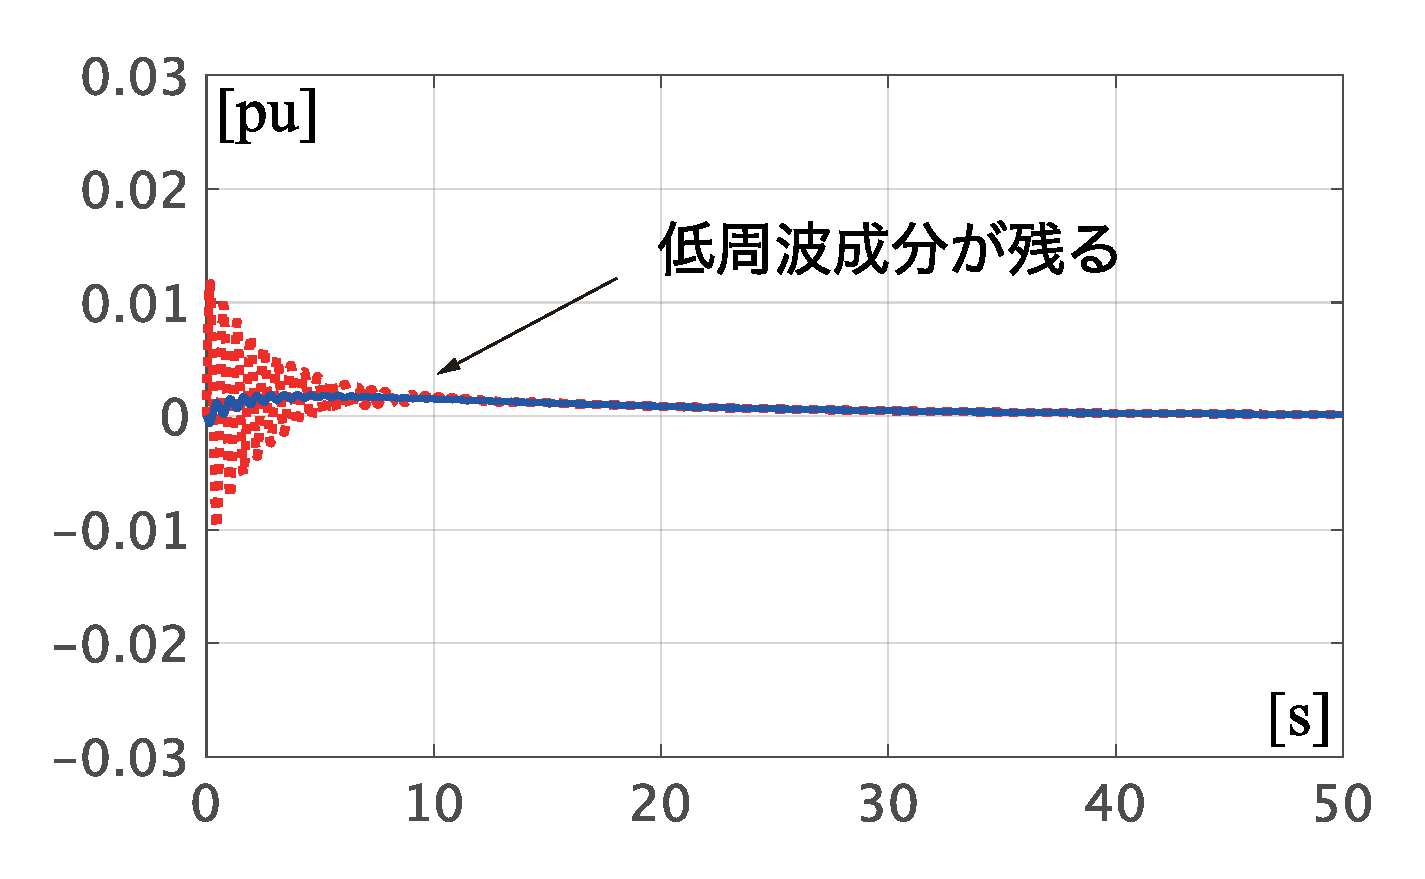
\includegraphics[width = 1.0\linewidth]{figs/woAVRsmall}
    \subcaption{Without AVR}
  \end{minipage}
  \begin{minipage}{0.49\linewidth}
    \centering
    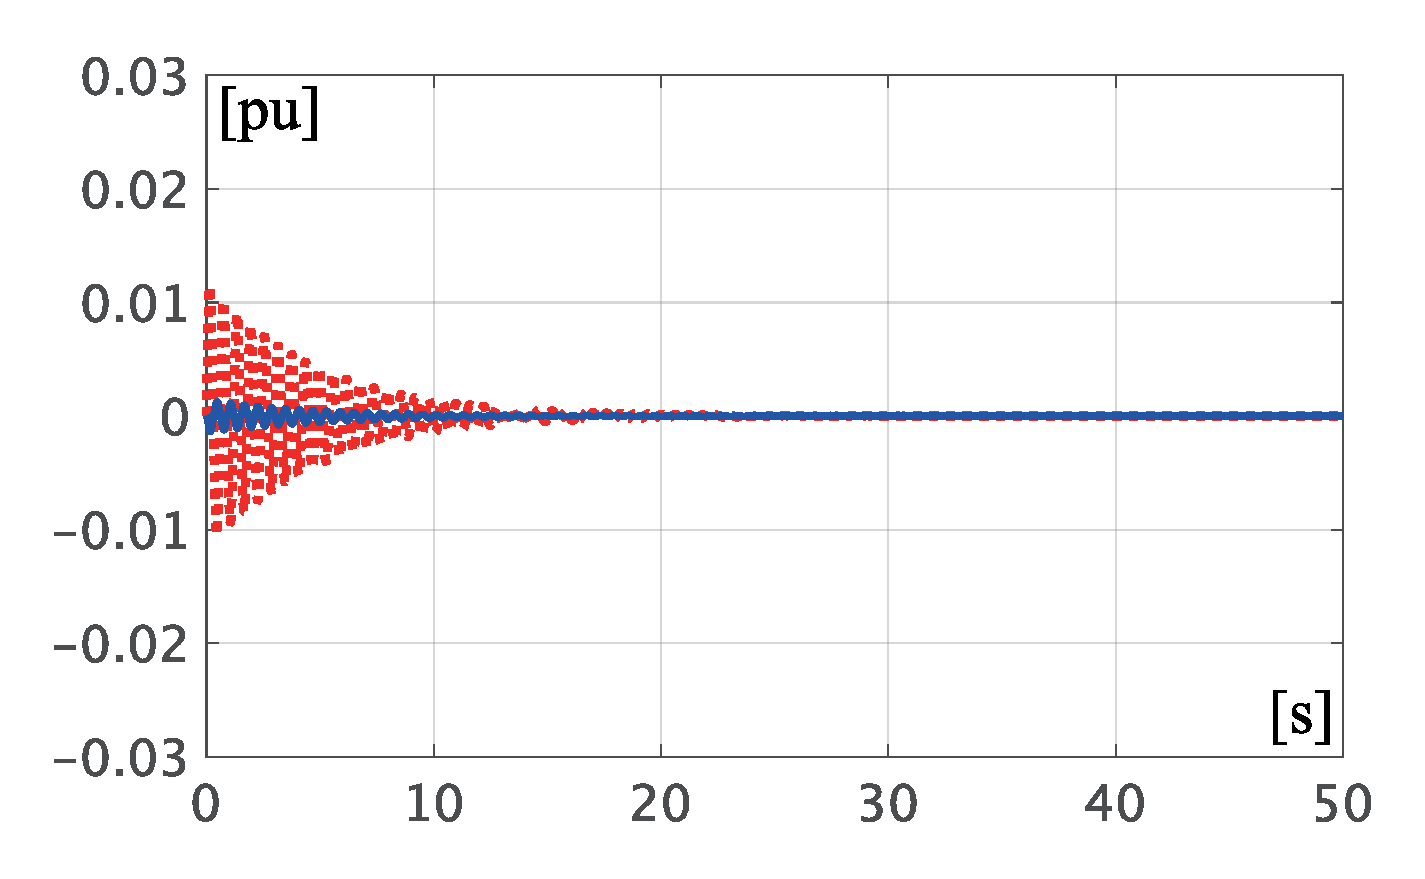
\includegraphics[width = 1.0\linewidth]{figs/wAVRsmall}
    \subcaption{With AVR}
  \end{minipage}
  \medskip
  \caption{\textbf{Initial value response of angular frequency deviation}
  \\ \centering{(Blue solid line: $\Delta\omega_1$, red dashed line: $\Delta\omega_3$)}
  }
  \label{fig:avrsmalld}
  }
\medskip
\end{figure}

\begin{figure}[t]
  \centering
  {
  \begin{minipage}{0.49\linewidth}
    \centering
    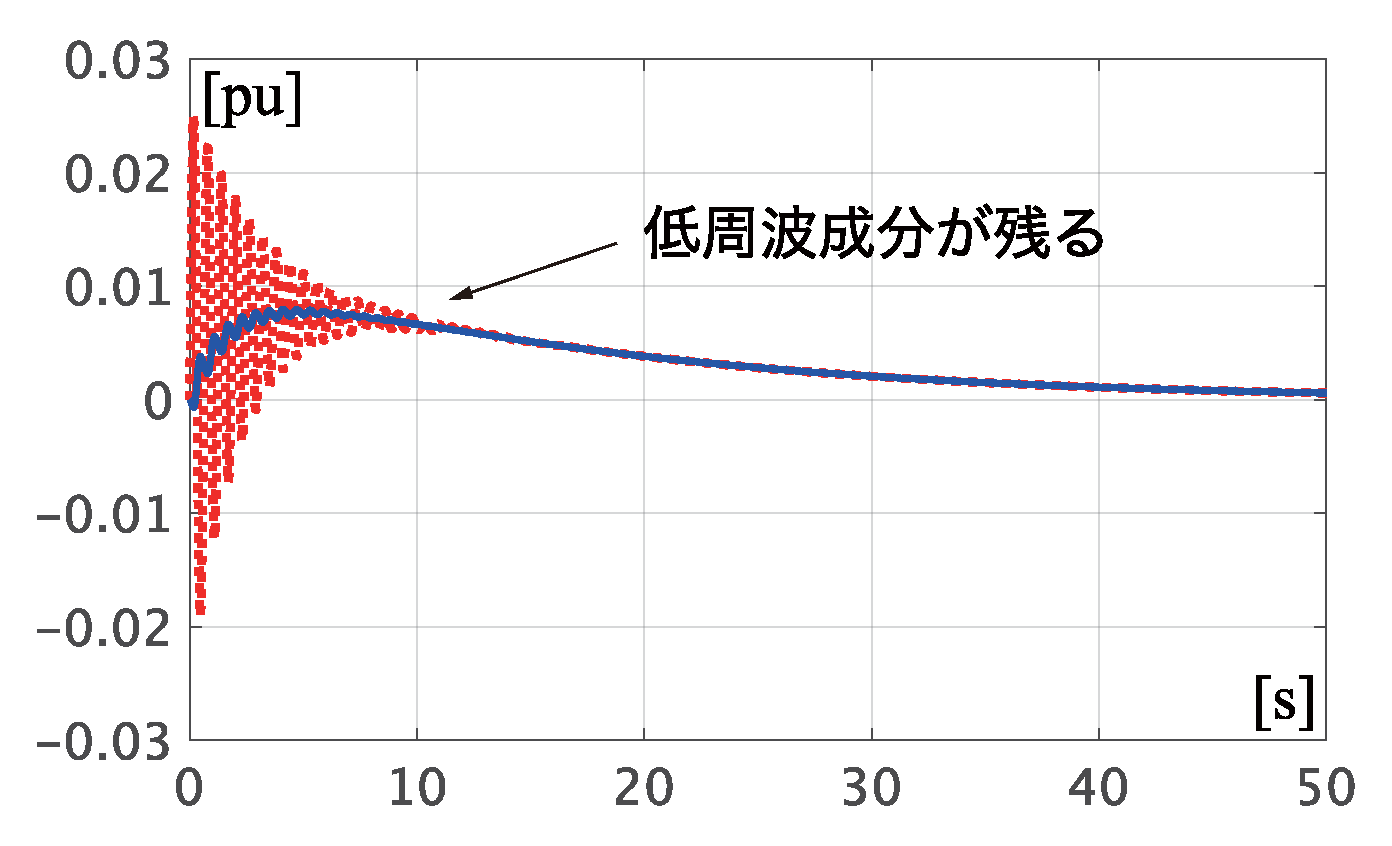
\includegraphics[width = 1.0\linewidth]{figs/woAVRlarge}
    \subcaption{Without AVR}
  \end{minipage}
  \begin{minipage}{0.49\linewidth}
    \centering
    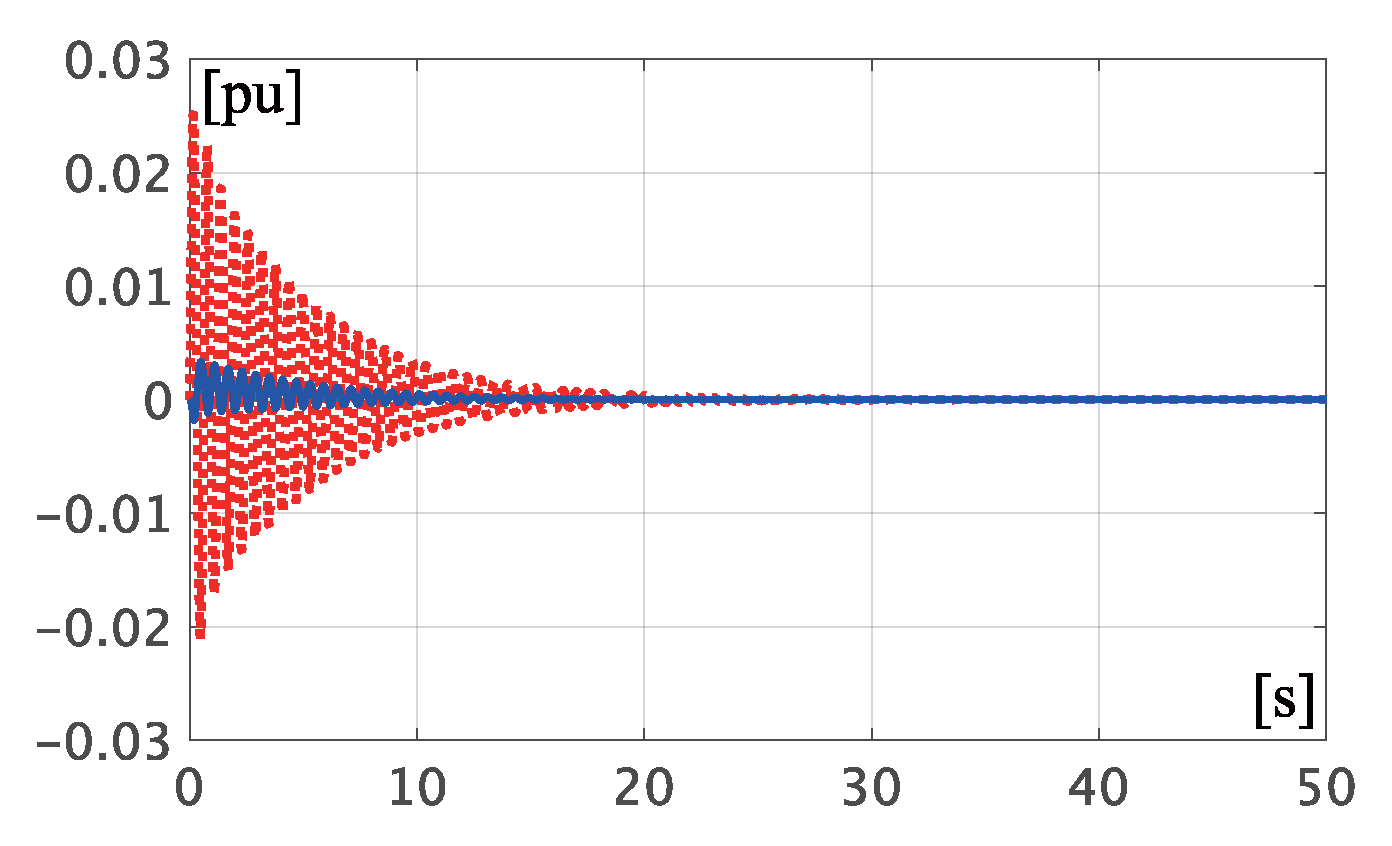
\includegraphics[width = 1.0\linewidth]{figs/wAVRlarge}
    \subcaption{With AVR}
  \end{minipage}
  \medskip
  \caption{\textbf{Initial value response of angular frequency deviation}
  \\ \centering{(Blue solid line: $\Delta\omega_1$, Red dashed line: $\Delta\omega_3$)} 
}
  \label{fig:avrlarged}
  }
\medskip
\end{figure}

From Example \ref{ex:avreffect}, it can be seen that incorporating an automatic
voltage regulator tends to destabilize some of the equilibrium points that were
stable before implementation, while suppressing the low-frequency components of
the oscillation of the angular frequency deviation. This means that the
transient stability of the power system has improved. The system stabilization
device described in the next section has the effect of suppressing the
high-frequency components of the oscillation that could not be suppressed by the
automatic voltage regulator.

\subsection{Power System Stabilizer}\label{sec:pssintro}

A power system stabilizer (PSS) is a device that outputs an additional control
signal $V_{\rm pss}$ as shown in Figures \ref{fig:avrdc1} and \ref{fig:avrst1}.
Generally, measurements such as generator's angular frequency deviation, active
power, and bus voltage phase are fed back to the PSS. Here we explain the model
of a standard PSS called the \textbf{IEEE Type PSS1 power system stabilizer
model}\index{IEEE Type PSS1 power system stabilizer model} \cite[Section
9.2]{ieee2016ieee}. This model mainly consists of two parts: a \textbf{washout
filter}\index{washout filter} and a \textbf{phase-lead
compensator}\index{phase-lead compensator}. The block diagram is shown in Figure 
\ref{fig:pss1}.

\begin{figure}[t]
  \centering
  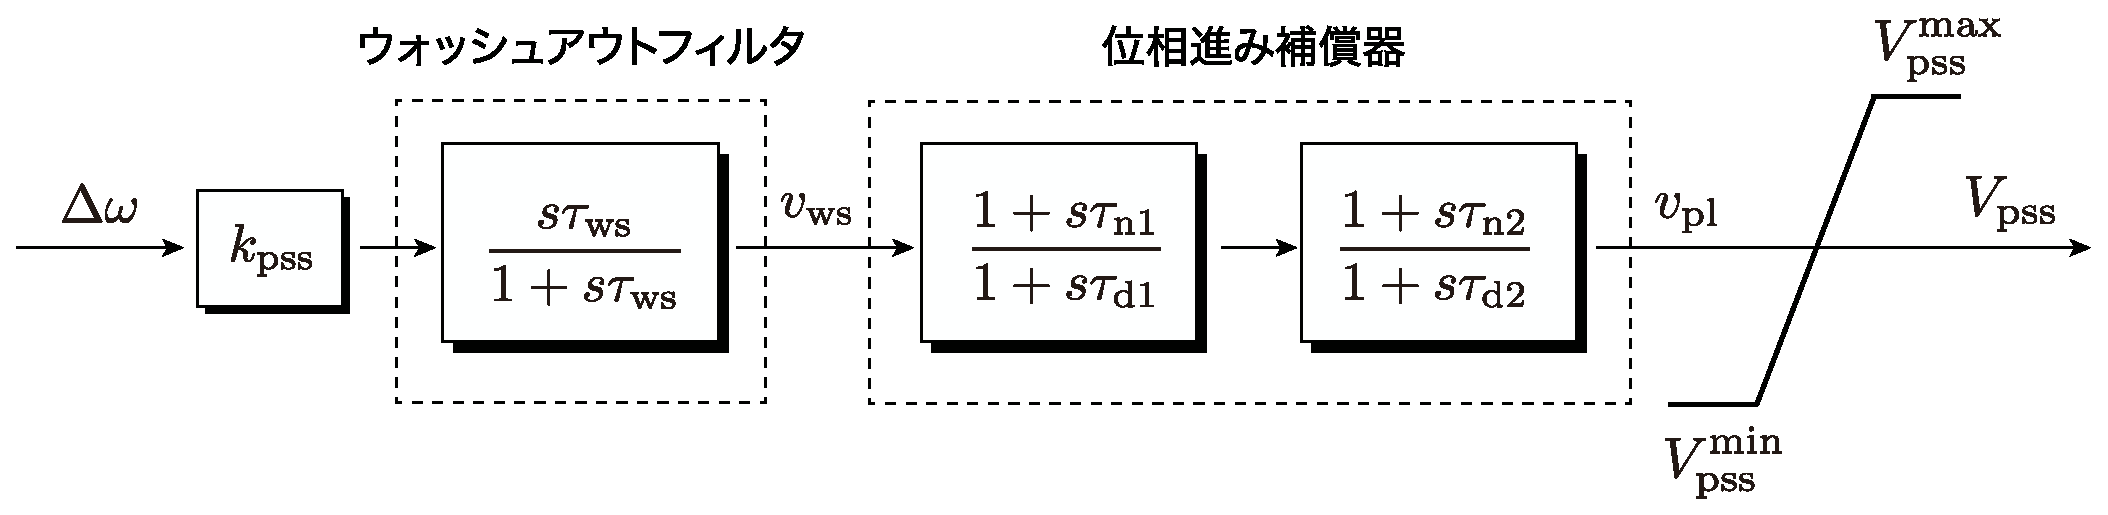
\includegraphics[width = .99\linewidth]{figs/pss1}
  \medskip
  \caption{\textbf{IEEE PSS1 type model of system stabilizer}}
  \label{fig:pss1}
  \medskip
\end{figure}


\smallskip
\subsubsection{Washout filter}

The washout filter is a high-pass filter used in the power system stabilizer to
maintain a steady-state gain of 0. It takes the generator's angular frequency
deviation $\Delta \omega$, which is multiplied by a constant gain $k_{\rm pss}$,
as input, and its dynamic characteristics are expressed by the following
differential equation:

\begin{subequations}\label{eq:pss1mod}
\begin{equation}\label{eq:washmod}
  \simode{
    \tau_{\rm ws} \dot{\xi}_{\rm ws} &=
    - \xi_{\rm ws}
    + k_{\rm pss} \Delta \omega \\
    v_{\rm ws} &= k_{\rm pss} \Delta \omega - \xi_{\rm ws}
  }
\end{equation}

The steady-state output $v_{\rm ws}^{\star}$ of the washout filter is zero when
the input $\Delta \omega$ is constant. The function of the filter is to extract
the angular frequency deviation of the power system in the transient state. The
time constant $\tau_{\rm ws}$ is typically set between 1 and 20 seconds,
considering the settling time of the angular frequency deviation
\cite[12.5]{kundur1994power}.

\smallskip
\subsubsection{Phase-lead compensator}

The phase-lead compensator is incorporated to alleviate the phase lag from the
bus voltage phase to the generator's active power. Typically, one or two phase
lead compensators are connected in series to achieve the desired phase lead.
Specifically, the dynamic characteristics of the compensator with input $v_{\rm
ws}$ from the washout filter is given by:

\begin{equation}\label{eq:phldmod}
  \simode{
  \tau_{{\rm d}1} \dot{\xi}_{1} &=
  - \xi_{1}
  + \left( 
  1- \tfrac{\tau_{{\rm d}1}}{\tau_{{\rm n}1}}
  \right)
  v_{\rm ws} \\
  v_{1} &= \tfrac{\tau_{{\rm n}1}}{\tau_{{\rm d}1}} (v_{\rm ws} - \xi_{1} )
  }
  \qquad
  \simode{
  \tau_{{\rm d}2} \dot{\xi}_{2} &=
  - \xi_{2}
  + \left( 
  1- \tfrac{\tau_{{\rm d}2}}{\tau_{{\rm n}2}}
  \right)
  v_{1} \\
  v_{\rm pl} &= \tfrac{\tau_{{\rm n}2}}{\tau_{{\rm d}2}} (v_{1} - \xi_{2} )
  }
\end{equation}

Finally, the output of the power system stabilizer can be obtained by applying
the output $v_{\rm pl}$ of the phase-lead compensator to a saturation function:

\begin{equation}\label{eq:psssat}
  V_{\rm pss} = \sfsat \left(
  v_{\rm pl};
  V_{\rm pss}^{\rm min},V_{\rm pss}^{\rm max} 
  \right)
\end{equation}
\end{subequations}

An example of the parameters for this model is shown in Table
\ref{table:psspara}. However, it should be noted that the parameters for the
power system stabilizer need to be determined by considering various factors
such as the dynamic characteristics of each generator, automatic voltage
regulator, load distribution, and characteristics of the transmission network,
and that the desired system stability may not necessarily be achieved by the
parameter settings shown in the example. In addition, the standard design
guidelines for power system stabilizers are often based on the one-machine
infinite-bus system model explained in Section \ref{sec:onemachine}, and caution
is required regarding the results when multiple generators are interconnected.
For example, in \cite[Section 12.5]{kundur1994power}, design guidelines for
parameters based on classical control theory using the one-machine infinite-bus
system model are presented.  In \cite{chow2004power}, design guidelines based on
modern control theory are also explained.

\begin{table}[ht]
\medskip
 \caption{\textbf{IEEE PSS1 type model parameter example}}
 \label{table:psspara}
 \centering
  \begin{tabular}{lccccccccccccc}
   \hline
 &  $k_{\rm pss}$ & $\tau_{\rm ws}$ & $\tau_{{\rm d}1}$ & $\tau_{{\rm n}1}$ & $\tau_{{\rm d}2}$ & $\tau_{{\rm n}2}$ & $V_{\rm pss}^{\rm min}$ & $V_{\rm pss}^{\rm min}$ \\
   \hline \hline
   Example 1 \cite[Section 12.5]{kundur1994power}& 9.50 & 1.4 & 0.033 & 0.154 & 0.00 & 0.00 & $-\infty$ & $\infty$ \\
   Example 2 \cite[Section 12.8]{kundur1994power}& 20.0 & 10.0 & 0.02 & 0.05 & 5.40 & 3.00 & $-\infty$ & $\infty$ \\
   Example 3 \cite[Section III]{chow2004power}& 1.57 & 10.0 & 0.03 & 0.34 & 0.03 & 0.34 & $-\infty$ & $\infty$ \\
   Example 4 \cite[Table H.3]{ieee2016ieee}& 3.15 & 10.0 & 0.01 & 0.76 & 0.01 & 0.76 & $-0.09$ & 0.09\\
   \hline
  \end{tabular}
\end{table}

\subsection{Control Effect of Power System Stabilization Device}\label{sec:pssov}

Let's analyze the control effect of the power system stabilization device using
a simple power system model.

\begin{example}{Changes in the small signal stability and the transient stability due to PSS}\label{ex:psseffect}

Let us consider incorporating a power system stabilization device into the
system along with an automatic voltage regulator under the same conditions as
Example \ref{ex:avreffect}. The power system stabilization devices installed in
generators 1 and 3 are identical, and the parameters use the values of Example 2
in Table \ref{table:psspara}. First, let us confirm the change in the set of
stable equilibrium points due to the presence of the power system stabilization
device, which is shown in the range of (iii) in Table \ref{table:stableeqs}. From
this result, it can be seen that the set of stable equilibrium points has
expanded by incorporating the power system stabilization device.

\end{example}

\begin{figure}[t]
  \centering
  {
  \begin{minipage}{0.49\linewidth}
    \centering
    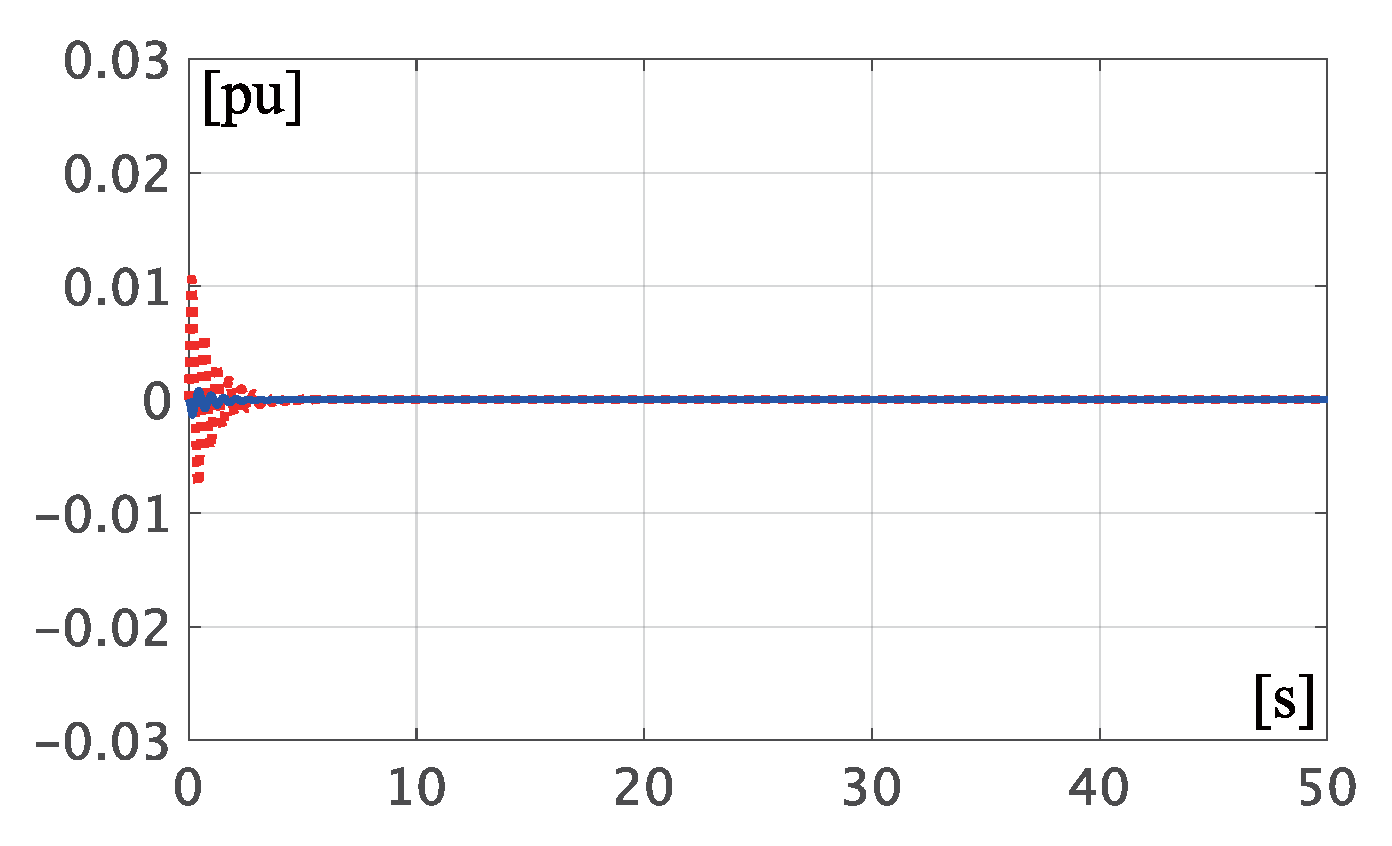
\includegraphics[width = 1.0\linewidth]{figs/wPSSsmall}
    \subcaption{ $\delta_1(0) - \delta_3(0) =-1$}
  \end{minipage}
  \begin{minipage}{0.49\linewidth}
    \centering
    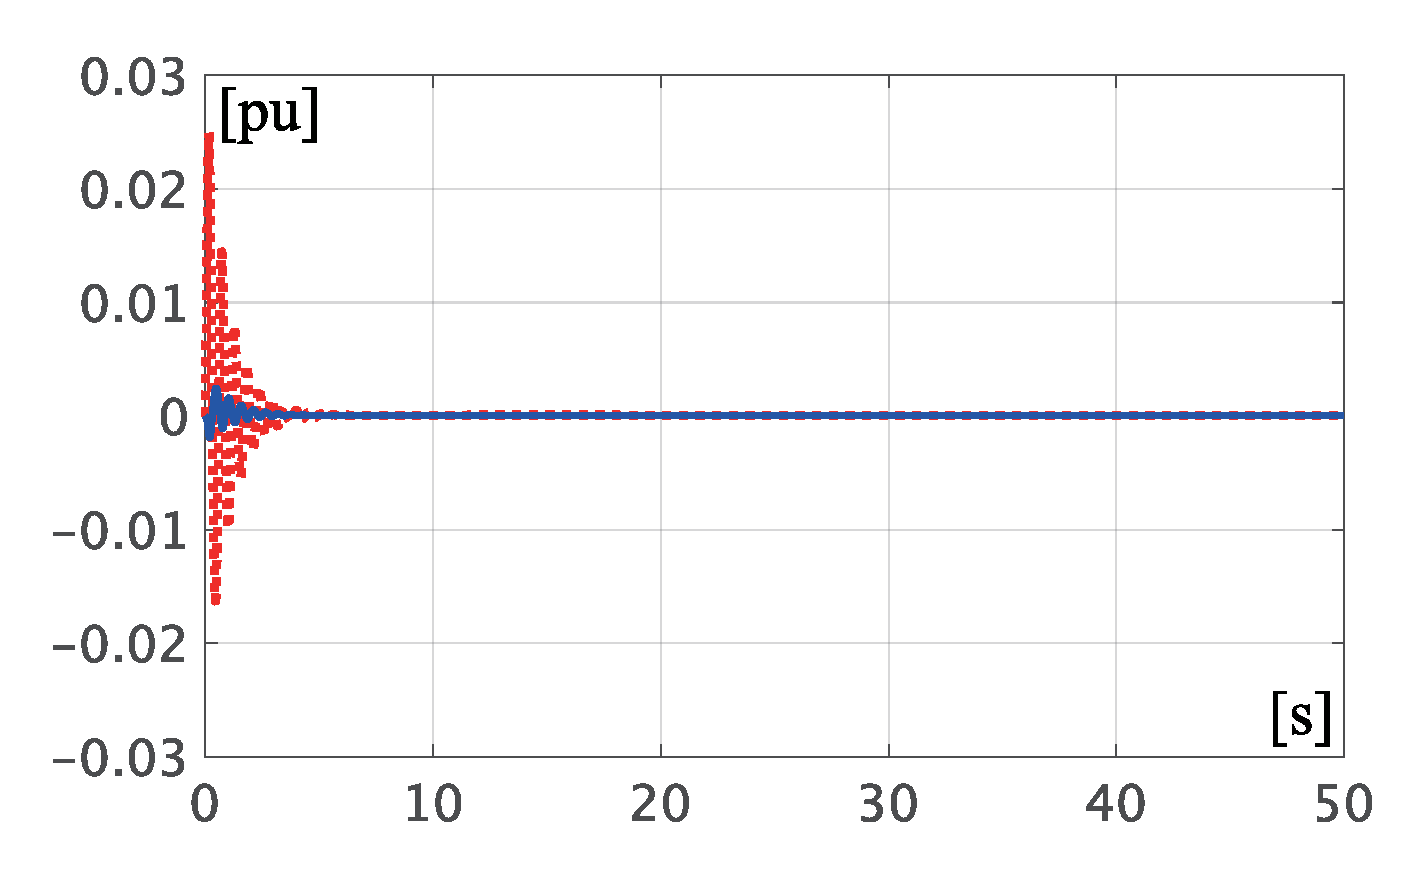
\includegraphics[width = 1.0\linewidth]{figs/wPSSlarge}
    \subcaption{ $\delta_1(0) - \delta_3(0) =-1.57$}
  \end{minipage}
  \medskip
  \caption{\textbf{Initial value response of angular frequency deviation}
  \\ \centering(There is a system stabilizer, and the line type is the same as \ref{fig: avrsmalld})}
  \label{fig:PSSomega}
  }
\medskip
\end{figure}

\section{PSS based on the retrofit control theory}\label{sec:retrofit}

\subsection{Power system model used in the design of PSS}

\smallskip
\subsubsection{Features of PSS based on the retrofit control theory}

In this section, we describe the design methodology of the power system
stabilizer based on retrofit control theory
\cite{ishizaki2018retrofit,sadamoto2018retrofit,sasahara2019damping,ishizaki2019retrofit,ishizaki2021modularity}.
The power system stabilizer designed using this methodology can maintain the
steady-state power flow condition in a stable manner even when multiple
generators are simultaneously incorporated. In particular, each power system
stabilizer has the following features:

\begin{itemize}
\item Distributed design is possible with just a mathematical model of generators and AVR that incorporates it.
\item Distributed implementation is possible with just the local measurement signal of the voltage phasor and current phasor of generator buses.
\end{itemize}

Next, we consider the case where the IEEE ST1 type AVR model in Equation
\ref{eq:avrst1} is incorporated into the generator model in Equation
\ref{eq:gendifavr}. However, for the sake of simplicity, we exclude saturation
of the AVR. Note that the same discussion applies not only to the case with
saturation but also to the case where other types of AVRs are incorporated, the
case where existing power system stabilizers are incorporated, and the case
where a more detailed generator model is used.

\smallskip
\subsubsection{Localized linear subsystem}
By designing the interaction inputs appropriately, we consider representing the
local subsystem, which is coupled with an AVR of the target generator, as a
linear system in the form of:

\begin{equation}\label{eq:desmodl}
  G:\simode{
  \dot{x} &= Ax + Bu + Lv \\
  w &= \mathit{\Gamma} x \\
  y &= Cx
  }
\end{equation}
where the state vector $x$ is a concatenation of the states of the generator
model $\delta$, $\Delta \omega$, $E$, and the AVR model $V_{\rm tr}$.

In addition, the input $u$ represents the output $V_{\rm pss}$ of the PSS, and
the input-output interactions $v$ and $w$ are defined as:

\begin{equation}\label{eq:sigintvw}
  v:=
  \mat{
  P_{\rm mech} - \tfrac{E |\bm{V} |}{ \Xt } \sfsin(\delta -  \angle \bm{V}) \\
  k_{\rm ap} V_{\rm ref}^{\star} + 
  \left(
  \tfrac{ \Xs }{ \Xt }-1
  \right)
  |\bm{V}| \sfcos (\delta - \angle \bm{V} )\\
  |\bm{V}|
  }
  ,\qquad
  w:=\mat{
  \delta \\
  \Delta \omega \\
  E 
  }
\end{equation}

Note that the interaction input $v$ in Equation \ref{eq:sigintvw} contains the
non-linear terms of the generator and the variables of the bus voltage phase. It
should be noted that the system matrix in Equation \ref{eq:desmodl} is defined
in accordance with the definitions of these signals as follows:

\begin{equation}\label{eq:matlocalm}
  \spliteq{
    A&:=\mat{
    0 & \omega_0 & 0 & 0 \\
    0 & -\tfrac{D}{M} & 0 & 0 \\
    0 & 0 & -\tfrac{ \Xs }{ \taud \Xt } & -\tfrac{k_{\rm ap}}{ \taud } \\
    0 & 0 & 0 & -\tfrac{1}{\tau_{\rm tr}}
    }, \quad
    B:=
    \mat{
    0 \\
    0 \\
    \tfrac{k_{\rm ap}}{ \taud } \\
    0 
    },\quad
    C:= I \\
    L &:=
    \mat{
    0 & 0 & 0 \\
    \tfrac{1}{M} & 0 & 0 \\
    0 & \tfrac{1}{ \taud } & 0 \\
    0 & 0 & \tfrac{1}{\tau_{\rm tr} }
    }, \quad
    \mathit{\Gamma} :=
    \mat{
    1 & 0 & 0 & 0 \\
    0 & 1 & 0 & 0 \\
    0 & 0 & 1 & 0 
    }
  }
\end{equation}

The $G$ in Equation \ref{eq:desmodl} is called a \textbf{local linear
subsystem}. It should be noted that the nonlinear terms of the generator and the
variables of the bus voltage phase are included in the interaction input $v$ in
Equation \ref{eq:sigintvw}. The system matrix of Equation \ref{eq:matlocalm} is
defined for the local linear subsystem. The model parameters of the local linear
subsystem, i.e., the system matrix parameters in Equation \ref{eq:matlocalm},
are assumed to be known and available for the design and implementation of the
power system stabilizer.

\smallskip
\subsubsection{Environment and approximate linear environment model}

Let us consider designing a local controller $K$ for the power system stabilization
device, under the assumption that the output $y$ and interaction input/output
$v$ and $w$ are measurable.

\[
  K : (y,v,w)\mapsto u
\]

In the following, we call this controller $K$ a \textbf{retrofit
controller}\index{retrofit controller}, which derives from the words retroactive
and refit and refers to performing partial expansion or reconstruction of an
existing system.

In designing and implementing the retrofit controller, not only the model of the
local linear subsystem $G$ is used, but also a linear model that estimates the
interaction input $v$ from the interaction output $w$ is utilized. We call this
estimation model an \textbf{approximate linear environment
model}\index{approximate linear environment model}.

\begin{figure}[t]
  \centering
  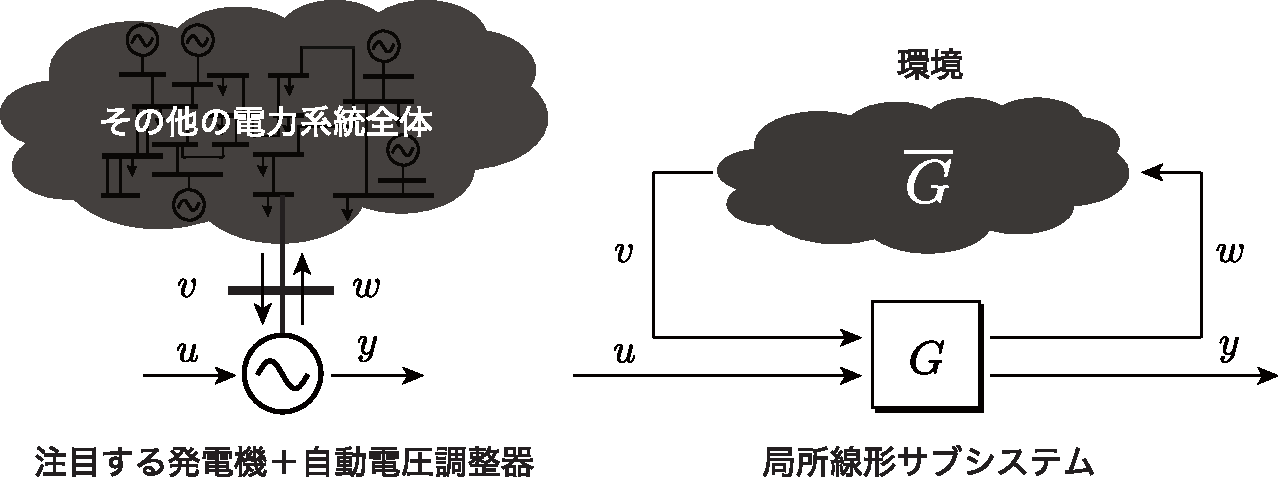
\includegraphics[width = .99\linewidth]{figs/retconsys2}
  \medskip
  \caption{\textbf{Coupling system of local linear subsystem and environment}}
  \label{fig:retconsys}
  \medskip
\end{figure}

To explain the approximate linear environment model, we introduce a nonlinear
subsystem called the \textbf{environment} \index{environment}, which represents
the global subsystem of the entire system except for the local linear subsystem.
The environment is a nonlinear system that takes the interaction output $w$ of
the local linear subsystem as input and outputs the interaction input $v$.
Formally, we represent the dynamic input-output relationship of the environment
as:

\[
  \overline{G}: w \mapsto v
\]

In this case, the feedback coupling system between the local linear subsystem
$G$ and the environment $\overline{G}$ represents the entire power system from
the perspective of the generator under consideration, as shown in Figure
\ref{fig:retconsys}.

Considering that the environment $\overline{G}$ includes numerous elements such
as power transmission networks, loads, and other generators, it is not practical
to assume that the complete nonlinear model of the environment is available for
the design and implementation of a system stabilizing device for a specific
generator. Taking this fact into consideration, let us assume a situation where
only an approximate linear model of the environment is available. For
simplicity, we will describe the approximate linear environment model using a
static input-output relationship. However, it is also possible to use a dynamic
approximate linear environment model. For further details, please refer to
\cite{ishizaki2019retrofit}.

When the steady-state values of the input-output interaction in the steady-state
power flow state of interest are denoted as $(v^{\star}, w^{\star})$, the
approximated linearized environmental model is parameterized as follows:

\begin{equation}\label{eq:Gbapxst}
  \overline{G}_{\rm apx}:
  v_{\rm apx} = v^{\star} + \overline{\mathit{\Theta}} \left(w-w^{\star}\right)
\end{equation}

Here, $\overline{\mathit{\Theta}}$ is a matrix representing the parameters of
the model. The approximated linearized environmental model $\overline{G}_{\rm
apx}$ in Equation \ref{eq:Gbapxst} generates the predicted value $v_{\rm apx}$ of
the impact of the interaction output $w$ on the interaction input $v$ in the
vicinity of their steady-state values $(v^{\star},w^{\star})$ by linear
prediction.

The power system model used for retrofit controller design is constructed by
feedback coupling the parameters of this approximated linearized environmental
model $\overline{\mathit{\Theta}}$ with the model of a local linear subsystem
$G$ as shown in Figure \ref{fig:explocalG}. Specifically, it is given by:

\begin{equation}\label{eq:Gplus}
  G^+: \begin{aligned} 
    \dot{\hat{\xi}} &=  \left( A+L \overline{\mathit{\Theta}} 
    \mathit{\Gamma} \right) \hat{\xi} + B \hat{u} \\
    \hat{y} & = C \hat{\xi}
  \end{aligned}
\end{equation}

Here, $\hat{u}$ and $\hat{y}$ are virtual input-output signals used for
controller design, and are distinguished from $u$ and $y$ by the use of a hat
symbol. Note that since $C$ is the identity matrix in Equation
\ref{eq:matlocalm}, the output $\hat{y}$ is equal to the internal state
$\hat{\xi}$ of $G^+$.

\begin{figure}[t]
\centering
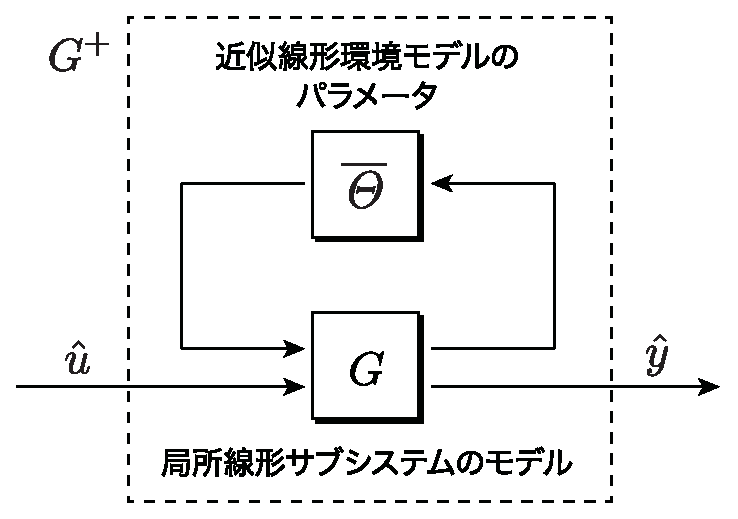
\includegraphics[width = .50\linewidth]{figs/explocalG2}
\medskip
\caption{\textbf{Model used for controller design}}
\label{fig:explocalG}
\medskip
\end{figure}

\subsection{PSS design based on the retrofit control theory}\label{sec:designret}

\smallskip
\subsubsection{Design method of retrofit controller}

Assuming that the approximate linear environment parameter
$\overline{\mathit{\Theta}}$ in Equation \ref{eq:Gbapxst} is identified by an
appropriate method, we explain the design method of the retrofit controller. The
specific construction method of the approximate linear environment model is
described in the next section.

The design of the retrofit controller corresponding to the system stabilization
device can utilize the standard control system design method in the field of
system control engineering. For instance, let us apply the design method of the
\textbf{Linear Quadratic Regulator} (LQR) \index{Linear Quadratic Regulator}
\cite[Section 5.3]{fairman1998linear} to the controller design model $G^+$ in
Equation \ref{eq:Gplus}. In LQR, we use a state-feedback form control algorithm
that minimizes the cost function on state and input as follows:

\[
  J(\hat{\xi},\hat{u}) :=\int_0^{\infty} \left(
  \hat{\xi}^{\sf T}(t) Q \hat{\xi}(t)
  +
  \hat{u}^{\sf T}(t) R \hat{u}(t)
  \right) dt
\]

Using the state feedback form in equation \ref{eq:locKhat}:

\begin{equation}\label{eq:locKhat}
  \hat{u}=\underbrace{-R^{-1}B^{\sf T}P(\overline{\mathit{\Theta}}) }_{\hat{K}(\overline{\mathit{\Theta}}) }
  \hat{\xi}
\end{equation}


Here, $Q$ is a semi-positive definite matrix, $R$ is a positive definite matrix,
and the matrix $P(\overline{\mathit{\Theta}})$ satisfies the \textbf{Algebraic
Riccati Equation} \index{Algebraic Riccati Equation} as follows:

\[
  \left( A+L \overline{\mathit{\Theta}} 
  \mathit{\Gamma} \right)^{\sf T} P +
  P \left( A+L \overline{\mathit{\Theta}} 
  \mathit{\Gamma} \right)
  -PB R^{-1} B^{\sf T} P +Q = 0
\]

This equation has a positive definite solution. Then, using the gain matrix
$\hat{K}(\overline{\mathit{\Theta}})$ in Equation \ref{eq:locKhat}, the retrofit
controller is constructed as follows:

\begin{equation}\label{eq:retroK}
K: \begin{aligned}
  \dot{\hat{x}} &=  A \hat{x} + L \left\{
  v - \overline{\mathit{\Theta}} (w- \mathit{\Gamma} \hat{x}) 
  \right\}\\
  u &= \hat{K}(\overline{\mathit{\Theta}}) (y - C\hat{x})
  \end{aligned} 
\end{equation}

Based on this retrofit control theory, the system stabilization device has the
following characteristics for any matrix $\overline{\mathit{\Theta}}$:

\begin{itemize}
  \item When the power system is in steady-state, the input $u$ becomes zero.
  \item The stability of the steady-state (equilibrium point) does not change before and after implementation.
\end{itemize}

The first item means that the retrofit controller does not change the
steady-state condition, while the second item means that the implementation of
the retrofit controller does not change an asymptotically stable equilibrium
point to an unstable one. The objective of retrofit control theory is to improve
stability while maintaining the asymptotic stability of the equilibrium point
and using indicators such as robustness to disturbances and the size of the
stability region. Note that this method cannot asymptotically stabilize an
unstable equilibrium point before controller implementation.

Furthermore, it has been shown that the larger the predictive accuracy of the
interaction signal by the approximate linear environmental model, the greater
the improvement in system stability. Note that if the control algorithm in
equation \ref{eq:locKhat} stabilizes $G^+$ in equation \ref{eq:Gplus}, it is not
necessary to use the linear quadratic regulator (LQR) method introduced in
section 5.3 of \cite{fairman1998linear}. Additionally,
$\hat{K}(\overline{\mathit{\Theta}})$ can be a dynamic control algorithm, and it
does not need to be static \cite{ishizaki2019retrofit}.

\smallskip
\subsubsection{Construction method of approximate linear environmental model}

One practical approach for identifying the parameter
$\overline{\mathit{\Theta}}$ in Equation \ref{eq:Gbapxst} is to estimate the
relationship between the signals $w$ and $v$ using linearization. Specifically,
the partial derivatives of $v$ with respect to each element of $w$ are
calculated as:

\begin{equation}
  \spliteq{
    \frac{\partial v }{\partial \delta} &= 
    \mat{
    - \tfrac{E |\bm{V} |}{ \Xt } \sfcos(\delta -  \angle \bm{V})  \\
    - \left( \tfrac{\Xs }{ \Xt }-1 \right)
    |\bm{V}| \sfsin (\delta - \angle \bm{V} ) \\
    0
    }
    , \qquad
    \frac{\partial v }{\partial \Delta \omega} = \mat{0 \\0\\0} \\
    \frac{\partial v }{\partial E} &= 
    \mat{
    - \tfrac{|\bm{V} |}{ \Xt } \sfsin(\delta -  \angle \bm{V}) \\
    0\\
    0
    }
  }
\end{equation}

Therefore, assuming that the internal state of the generator and the voltage
phase of the generator bus are in the vicinity of the steady-state conditions,
we obtain:

\begin{equation}\label{eq:basenvm}
  \overline{\mathit{\Theta}}^{\rm int} :=
  \mat{
    - \tfrac{E^{\star} |\bm{V}^{\star} |}{ \Xt } \sfcos(\delta^{\star} -  \angle \bm{V}^{\star}) &
    0   & 
    - \tfrac{|\bm{V}^{\star} |}{ \Xt } \sfsin(\delta^{\star} -  \angle \bm{V}^{\star})
    \\
    - \left( \tfrac{ \Xs }{ \Xt }-1 \right) 
    |\bm{V}^{\star}| \sfsin (\delta^{\star} - \angle \bm{V}^{\star} ) 
    & 0 
    & 0 
    \\
    0 & 0 &0
  }
\end{equation}

Here, the steady-state values of the internal state $(\delta^{\star},E^{\star})$
of the generator and the steady-state value of the bus voltage phase
$(|\bm{V}^{\star}|,\angle \bm{V}^{\star})$ are the same as those of
$(v^{\star},w^{\star})$ in Equation \ref{eq:Gbapxst} under the steady-state
conditions. By using the matrix $\overline{\mathit{\Theta}}^{\rm int}$ in
Equation \ref{eq:basenvm}, we can model the "local feedback structure that the
internal state of the generator itself exerts". Since the normal power system
is operated in the vicinity of the steady-state conditions, the steady-state
values required for modeling can be identified based on measured data.

Next, let's consider estimating the indirect effect that signal $w$ has on
signal $v$ through automatic generation control. The partial derivative of $v$
with respect to the input $P_{\rm mech}$ of automatic generation control is
given by:

\[
  \frac{\partial v}{\partial P_{\rm mech}}
  =
  \mat{
  1\\0\\0
}
\]

When the broadcast-type PI controller in Equation \ref{eq:agccon} is
incorporated as automatic generation control, the time integral of $\omega_0
\Delta \omega$ corresponds to $\delta$, so we have:

\[
  \frac{\partial P_{\rm mech}}{\partial \delta} = -  \frac{\alpha \beta k_{\rm I}}{\omega_0} 
  ,\qquad
  \frac{\partial P_{\rm mech}}{\partial \Delta \omega}= - \alpha \beta k_{\rm P}
  ,\qquad
  \frac{\partial P_{\rm mech}}{\partial E}= 0
\]

Therefore, by the chain rule of differentiation, the effect of signal $w$ on
signal $v$ through the broadcast-type PI controller can be modeled as:

\begin{equation}
  \overline{\mathit{\Theta}}^{\rm agc}:=
  -  \alpha \beta \mat{
  \tfrac{k_{\rm I}}{\omega_0} & k_{\rm P}  & 0\\
  0 & 0 & 0\\
  0 & 0 & 0
  }
\end{equation}

Note that to obtain this parameter, it is necessary to obtain the values of the
controller gains for automatic generation control through an appropriate method.

Similarly, let us consider estimating the indirect effect of signal $w$ on
signal $v$ through the bus voltage phasor $\bm{V}$.  The partial derivatives of
$v$ with respect to the voltage phasor variables $(|\bm{V}|,\angle \bm{V})$ are
given by:

\begin{equation}
  \spliteq{
    \frac{\partial v }{\partial |\bm{V}|} &= 
    \mat{
    -\tfrac{E }{ \Xt } \sfsin(\delta -  \angle \bm{V})  \\
    \left( \tfrac{ \Xs }{ \Xt }-1 \right)
    \sfcos (\delta - \angle \bm{V} ) \\
    1
    }
    \\
    \frac{\partial v }{\partial \angle \bm{V}} &= 
    \mat{
    \tfrac{E|\bm{V} |}{ \Xt } \sfcos(\delta -  \angle \bm{V}) \\
    \left( \tfrac{ \Xs }{ \Xt }-1 \right)
    |\bm{V}|\sfsin (\delta - \angle \bm{V} ) \\
    0
    }
  }
\end{equation}

On the other hand, as analyzed in Section \ref{sec:allgen}, the bus voltage
phase not only depends on the internal state of the connected generator but also
on the internal states of all other generators. Specifically, let
$\overline{\delta}$ and $\overline{E}$ denote the vector of internal states of
all generators except the one of interest. Then, the four partial derivatives
$\tfrac{\partial |\bm{V}| }{\partial \delta}$, $\tfrac{\partial \angle \bm{V}
}{\partial \delta}$, $\tfrac{\partial |\bm{V}| }{\partial E}$, and
$\tfrac{\partial \angle \bm{V} }{\partial E}$ depend on the vector $z_{\mathds
G}$ that combines the internal states of all generators as:

\[
  z_{\mathds G}:=(\delta,\overline{\delta},E,\overline{E})
\]

While it is difficult to obtain analytical expressions for these partial
derivatives for general power system models, if we can measure the numerical
values of the following matrix in the neighborhood of the steady-state power
flow $z_{\mathds G}^{\star}$ using measurement data:

\begin{equation}\label{eq:thetaV}
  \theta
  :=
  \mat{
  \tfrac{\partial |\bm{V}| }{\partial \delta}(z_{\mathds G}^{\star}) &
  0 &
  \tfrac{\partial |\bm{V}| }{\partial E}(z_{\mathds G}^{\star}) \\
  \tfrac{\partial \angle \bm{V} }{\partial \delta}(z_{\mathds G}^{\star}) &
  0 &
  \tfrac{\partial \angle \bm{V} }{\partial E}(z_{\mathds G}^{\star})
  }
\end{equation}
then we can model the indirect effect of signal $w$ on signal $v$ through the
bus voltage phase $\bm{V}$ as:

\begin{equation}\label{eq:ThetaV}
  \overline{\mathit{\Theta}}^{\rm ext}:=
  \mat{
  -\tfrac{E^{\star} }{ \Xt } \sfsin(\delta^{\star} -  \angle \bm{V}^{\star}) 
  &
  \tfrac{E^{\star}|\bm{V}^{\star} |}{ \Xt } \sfcos(\delta^{\star} -  \angle \bm{V}^{\star}) 
  \\
  \left( \tfrac{ \Xs }{ \Xt }-1 \right)
  \sfcos (\delta^{\star} - \angle \bm{V}^{\star} )  
  &
  \left( \tfrac{ \Xs }{ \Xt }-1 \right)
  |\bm{V}^{\star}|\sfsin (\delta^{\star} - \angle \bm{V}^{\star} )
  \\
  1 & 0
  }
  \hat{\theta}
\end{equation}
where $z_{\mathds G}^{\star}$ in Equation \ref{eq:thetaV} denotes the
steady-state value of $z_{\mathds G}$.

The 0 element in the second column corresponds to $\frac{\partial
|\bm{V}|}{\partial \Delta \omega}$ and $\frac{\partial \angle \bm{V}}{\partial
\Delta \omega}$. Furthermore, $\hat{\theta}$ in Equation \ref{eq:ThetaV}
represents the identified value of $\theta$. $\overline{\mathit{\Theta}}^{\rm
ext}$ in Equation \ref{eq:ThetaV} models the "global feedback structure that the
internal state of the generator exerts on itself," in contrast to
$\overline{\mathit{\Theta}}^{\rm int}$ in Equation \ref{eq:basenvm}, which
models the local feedback structure.

It is necessary to identify the parameter $\hat{\theta}$ using data measured
during operation, as the power system must always be operated stably. In control
engineering, identifying subsystems within an operating feedback system is
called "closed-loop identification" \index{closed-loop identification}
\cite{ljung1998system}. Closed-loop identification is often more difficult than
identification when input excitation is possible, as it is generally not
possible to freely excite the input of the system being identified.

When using all the estimates obtained from the aforementioned linearization
approximations simultaneously, the model parameters in Equation \ref{eq:Gbapxst}
are composed of:

\begin{equation}\label{eq:Thetasum}
  \overline{\mathit{\Theta}}=
  \overline{\mathit{\Theta}}^{\rm int}+
  \overline{\mathit{\Theta}}^{\rm agc}+
  \overline{\mathit{\Theta}}^{\rm ext}
\end{equation}

As previously explained, the retrofit controller in Equation \ref{eq:retroK}
does not change the stability of the steady-state power flow for any matrix
$\overline{\mathit{\Theta}}$. However, to maintain the predicted accuracy of the
interaction signals obtained from the linearized environment model, it is
desirable to update $\overline{\mathit{\Theta}}$ at appropriate intervals to
respond to changes in the power flow state.

\begin{figure}[t]
  \centering
  {
  \begin{minipage}{0.49\linewidth}
    \centering
    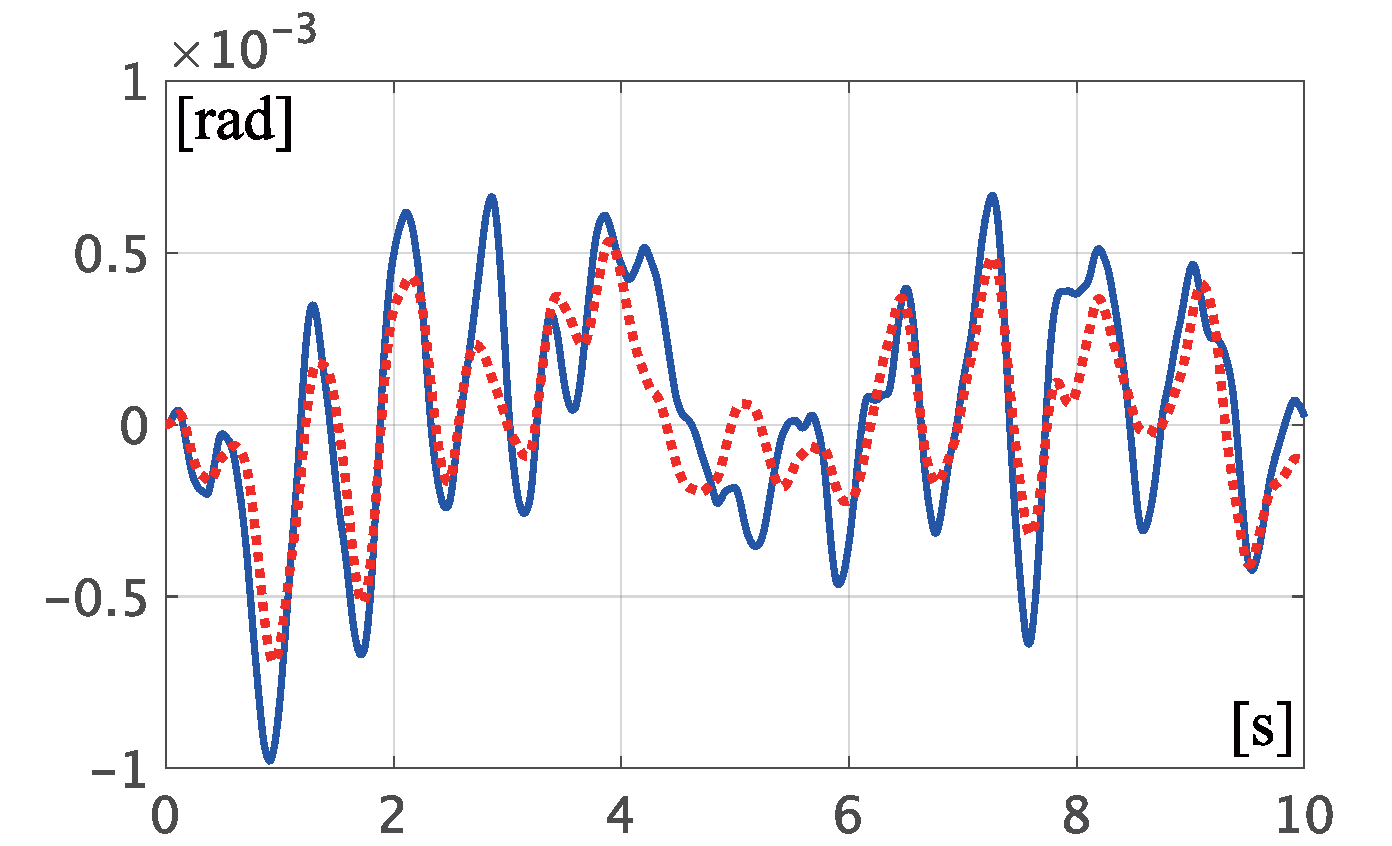
\includegraphics[width = 1.0\linewidth]{figs/timedeltamodel}
    \subcaption{Time series data of $\delta_3$ and $\hat{\delta}_3$}
     \medskip
  \end{minipage}
  \begin{minipage}{0.49\linewidth}
    \centering
    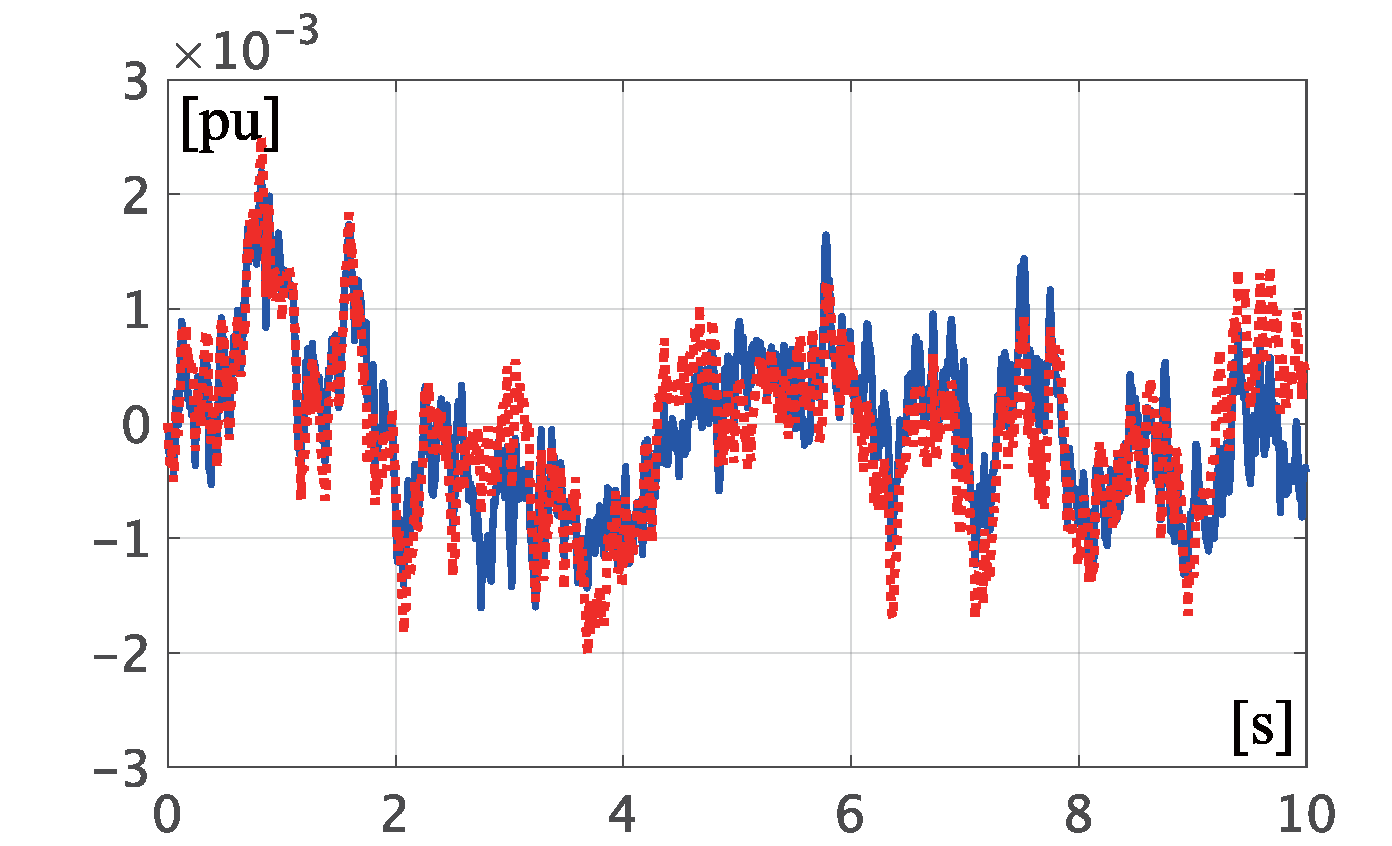
\includegraphics[width = 1.0\linewidth]{figs/timeEmodel}
    \subcaption{Time series data of $E_3$ and $\hat{E}_3$}
     \medskip
  \end{minipage}
    }
\caption{\textbf{Time response to random excitation input}
 \\ \centering(Blue solid line: $\delta_3, E_3$, Red dashed line: $\hat{\delta}_3,\hat{E}_3$)
 }
  \label{fig:timeVmodel}
\medskip
\end{figure}


\begin{figure}[t!]
  \centering
  {
  \begin{minipage}{0.49\linewidth}
    \centering
    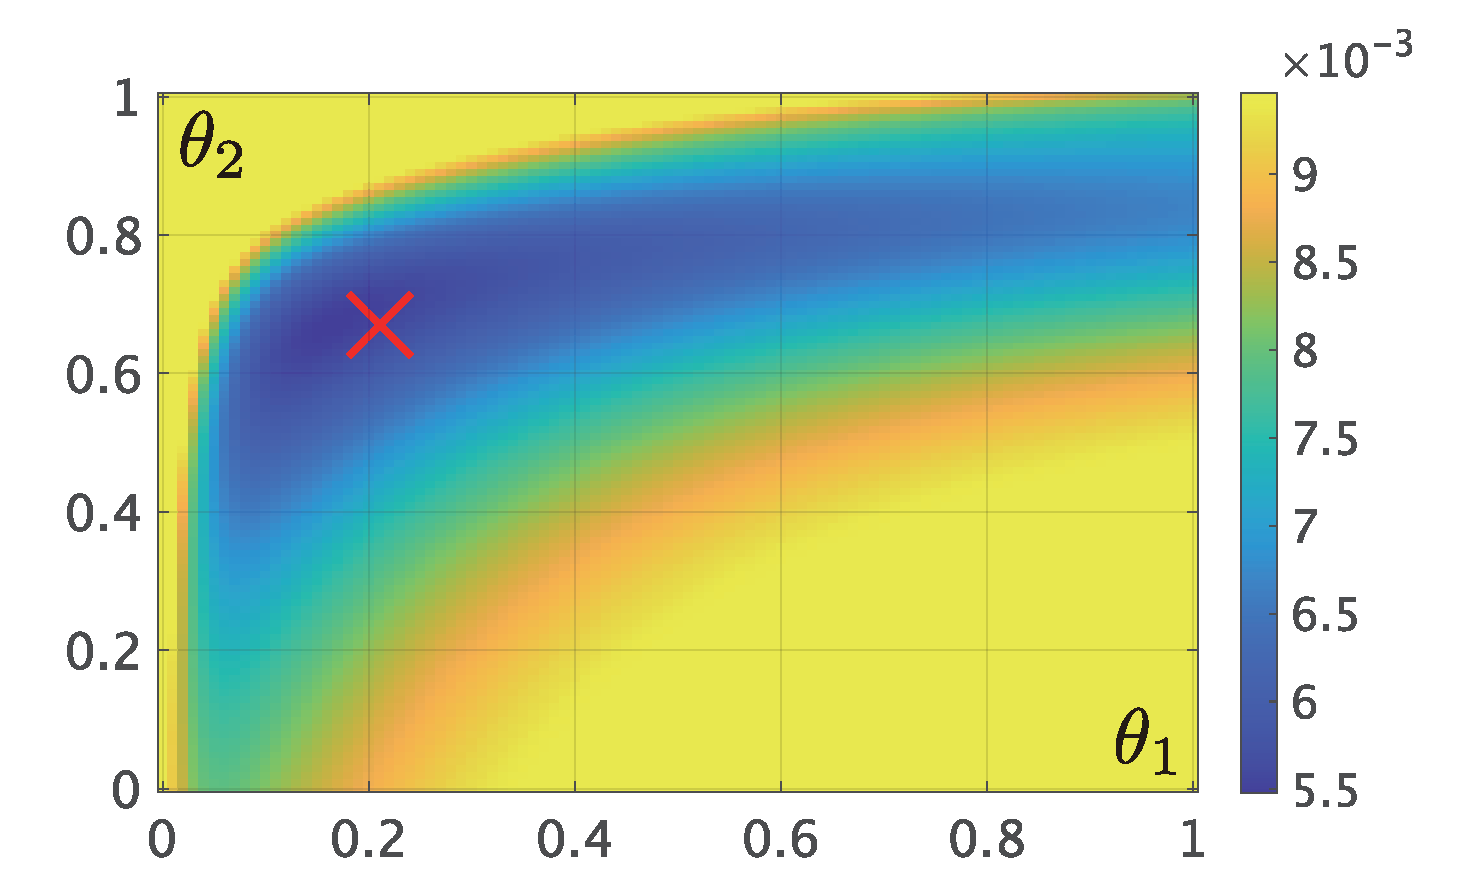
\includegraphics[width = 1\linewidth]{figs/heatdelta}
    \subcaption{ $Q(\delta_3,\hat{\delta}_3)$ }
    \medskip
  \end{minipage}
  \begin{minipage}{0.49\linewidth}
    \centering
    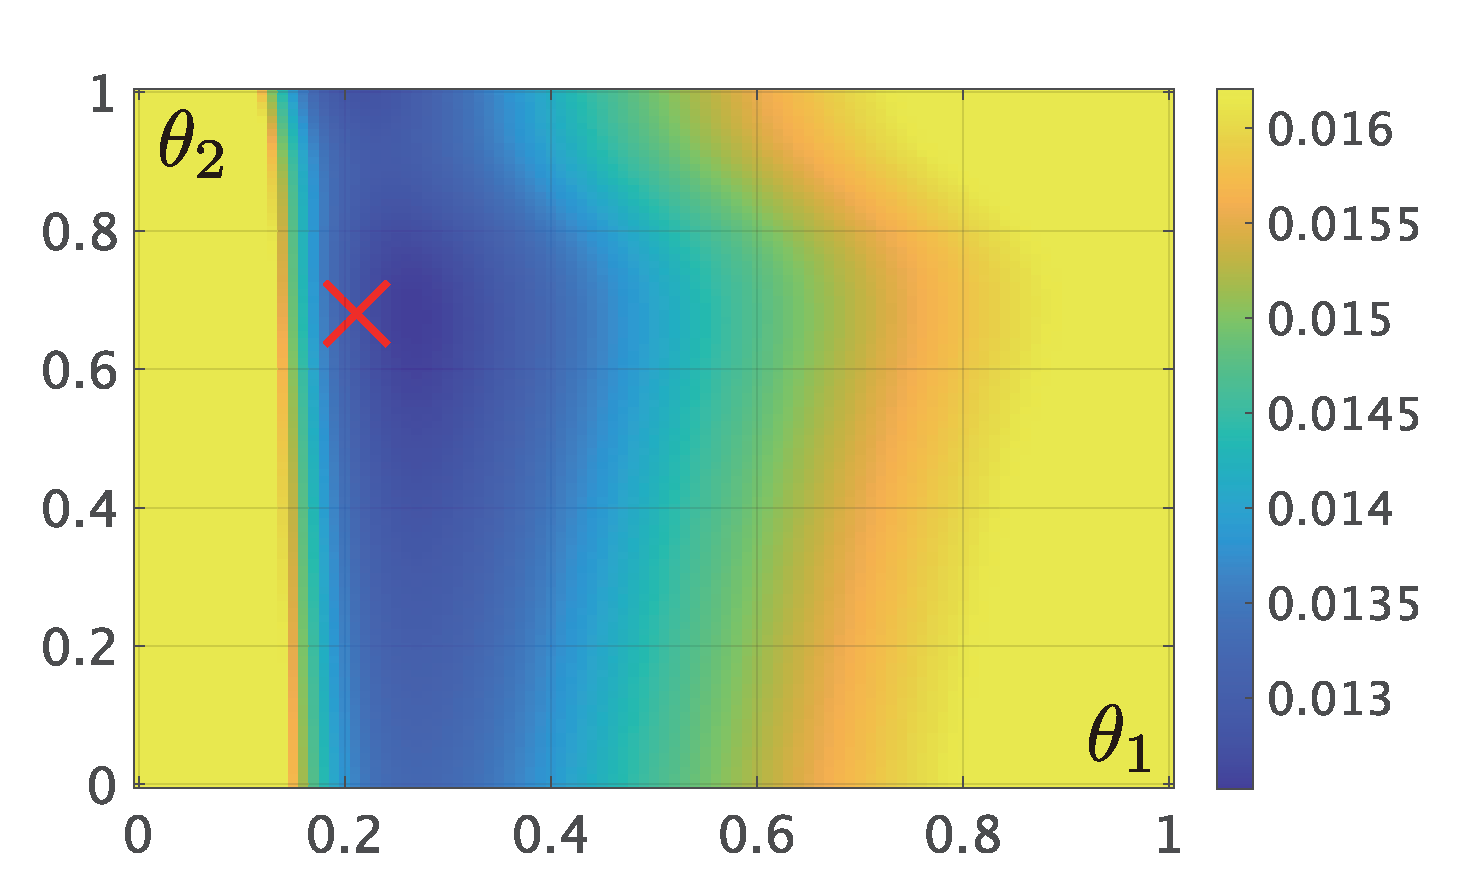
\includegraphics[width = 1\linewidth]{figs/heatE}
    \subcaption{ $Q(E_3,\hat{E}_3)$ }
    \medskip
  \end{minipage}
}
 \caption{\textbf{Approximation error of internal state with respect to identification parameter}}
 \label{fig:datamodeling}
\medskip
\end{figure}


\begin{example}{Identification of approximate linear environment model based on
measurement data}\label{ex:modelingV}

Similar to Example \ref{ex:avreffect}, we consider a power system model
consisting of three buses, with the same AVR incorporated into generators 1 and
3. We also assume that a broadcast-type PI controller with parameter values
given in Table \ref{table:agcpara}(b) is incorporated as automatic generation
control according to Equation (\ref{eq:agccon}). The steady-state power flow
condition corresponds to the results of the power flow calculation in Table
\ref{table:pflow2}.

In the following, we focus on generator 3 and identify the values of partial
derivatives of $\theta_3$ in Equation \ref{eq:thetaV} from measurement data.
However, the magnitudes of $\tfrac{\partial |\bm{V}3|}{\partial
\delta_3}(z{\mathds G}^{\star})$ and $\tfrac{\partial \angle \bm{V}3}{\partial
E_3}(z{\mathds G}^{\star})$ are relatively small, so we identify only two values
of $\theta_1$ and $\theta_2$ from the data, where:

\[
  \theta_1:=
  \frac{\partial | \bm{V}_3|}{\partial E_3}(z_{\mathds G}^{\star})
  ,\qquad
  \theta_2:=
  \frac{\partial \angle \bm{V}_3}{\partial \delta_3}(z_{\mathds G}^{\star})
\]

At this time, $\overline{\mathit{\Theta}}^{\rm ext}_3$ in Equation
\ref{eq:ThetaV} is parameterized as:

\begin{equation}\label{eq:Thext1para}
  \overline{\mathit{\Theta}}^{\rm ext}_3=
  \mat{
    \tfrac{E_3^{\star}|\bm{V}_3^{\star} |}{ \Xt_3 } \Delta^{\sf cos}_3 \theta_2
    & 
    0
    &
    - \tfrac{ E_3^{\star} }{ \Xt_3 } \Delta^{\sf sin}_3 \theta_1
    \\
    \left( \tfrac{ \Xs_3 }{ \Xt_3 }-1 \right)
    |\bm{V}_3^{\star}| \Delta^{\sf sin}_3 \theta_2
    &
    0
    &
    \left( \tfrac{ \Xs_3 }{ \Xt_3 }-1 \right)
    \Delta^{\sf cos}_3 \theta_1
    \\
    0 & 0 & \theta_1
  }
\end{equation}
where $\Delta^{\sf sin}_3$ and $\Delta^{\sf cos}_3$ are constants defined by:

\[
  \Delta^{\sf sin}_3 := \sfsin(\delta_3^{\star} -  \angle \bm{V}_3^{\star}) ,\qquad
  \Delta^{\sf cos}_3 := \sfcos (\delta_3^{\star} - \angle \bm{V}_3^{\star} )
\]

The optimization of the parameters $(\theta_1, \theta_2)$ is carried out using
the following procedure. Time series data of $(\delta_3, E_3)$ obtained by
randomly exciting the input $V_{{\rm pss}3}$ of the AVR is obtained from the
power system model. Furthermore, a controller design model $G_{3}^+$ for the
feedback system of the local linear subsystem $G_3$ and the approximate linear
environmental model parameters $\overline{\mathit{\Theta}}_3$ of Equation
\ref{eq:desmodl} is constructed for generator 3 using Equation \ref{eq:Gplus}.
Here, $\overline{\mathit{\Theta}}_3$ is defined by Equation \ref{eq:Thetasum}.
Then, time series data of $(\hat{\delta}_3, \hat{E}_3)$ are obtained as the
first and third elements of $\hat{y}3$ when the signal used to excite $V{{\rm
pss}3}$ is applied as the input $\hat{u}_3$ of Equation \ref{eq:Gplus}. The
parameters $(\theta_1, \theta_2)$ are optimized such that for all time instants
$t$ in the time interval where the data is obtained, $\hat{\delta}_3(t)$ and
$\hat{E}_3(t)$ are good approximations of $\delta_3(t)$ and $E_3(t)$,
respectively.

The time series data of $(\delta_3,E_3)$ is shown for the period from 0~[s] to
10~[s] when $V_{{\rm pss}3}$ is randomly excited, as indicated by the blue line
in Figure \ref{fig:timeVmodel}. However, the deviations from the steady-state
values $(\delta_3^{\star},E_3^{\star})$ are also shown. The results of an
exhaustive search for the optimal parameters $(\theta_1,\theta_2)$ on an evenly
spaced grid with a width of 0.01 for this data are shown in Figure
\ref{fig:datamodeling}. The horizontal and vertical axes represent the values
set for $\theta_1$ and $\theta_2$, respectively, and the colors in regions (a)
and (b) represent the values of the error functions $Q(\delta_3,\hat{\delta}_3)$
and $Q(E_3,\hat{E}_3)$, respectively.

Here, the error function $Q(x,\hat{x})$ is defined as follows:

\[
  Q(x,\hat{x}):=
  \sum_{k=1}^{1000}
  \left\|
  x\left(
  \tfrac{k}{100}
  \right)
  -
  \hat{x}\left(
  \tfrac{k}{100}
  \right)
  \right\|^2
\]

It evaluates the error of the continuous-time signal $x(t)$ for $t \in [0,10]$
with respect to the discrete-time signal $\hat{x}(t)$ sampled at 1,000 points
with a period of 0.01~[s].

Based on these results, the parameter values are set to $(0.215,0.675)$. Note
that this parameter value corresponds to the "x" mark in Figure
\ref{fig:datamodeling}. The time series data of $(\hat{\delta}_3,\hat{E}_3)$ for
this parameter setting is shown as the red dashed line in Figure
\ref{fig:timeVmodel}. It can be seen that the behavior of the internal state of
generator 3 is captured by the obtained approximate linear environment model.

\end{example}

In Example \ref{ex:modelingV}, the parameters of the approximate linear
environment model are identified as the index of the precision by which the
internal state of the generators is approximated. The effect of the retrofit
control based on this identification method is presented in Chapter
\ref{chap:largesim}.

\newpage
\end{document}